% notas:
% campo harmônico => harmonic field?
% anti-relative => counter-relative? (discussão sobre harmonia funcional)
%    associada relative => associated relative? (ver a discussão para mais...)
% medianas cromáticas => cromatic mediant
% tonalidade => key
% homônica => homonymous



\documentclass[
 aip,
 jmp,
 amsmath,amssymb,
 reprint,
]{revtex4-1}
\usepackage{graphicx}
\usepackage{grffile}
\usepackage{dcolumn}
\usepackage{bm}
\usepackage{multirow}
\usepackage{color}
\usepackage{xcolor}
\usepackage{enumerate}
\usepackage{float}

\newcommand{\massa}{{\large \textsc{massa}}}
\newcommand{\mass}{{\large \textsc{mass}}}
\newcommand{\figgus}{{\large \textsc{figgus}}}

\floatstyle{plain}
\newfloat{twocolequfloat}{t}{zzz}
\floatname{twocolequfloat}{Equation}


\begin{document}
\preprint{AIP/123-QED} 

\title{Psychophysics of musical elements in the discrete-time representation of sound}

\author{Renato Fabbri}
 \homepage{http://www.ifsc.usp.br/~fabbri}
 \email{renato.fabbri@gmail.com}
  \affiliation{ 
Instituto de F\'isica de S\~ao Carlos, Universidade de S\~ao Paulo (IFSC/USP)
}


\author{Vilson Vieira da Silva Jr.}
  \homepage{http://automata.cc/}
  \email{vilson@void.cc}
 \altaffiliation[Also at ]{IFSC-USP}


\author{D\'ebora Corr\^ea}
  \homepage{}
  \email{debcris.cor@gmail.com}
 \altaffiliation[Instituto de Ci\^encias Matem\'aticas e de Computa\c{c}\~ao ]{ICMC-USP}


\author{Luciano da Fontoura Costa}
  \homepage{http://cyvision.ifsc.usp.br/~luciano/}
  \email{ldfcosta@gmail.com}
 \altaffiliation[Also at ]{IFSC-USP}

 \author{Osvaldo N. Oliveira Jr.}
  \homepage{www.polimeros.ifsc.usp.br/professors/professor.php?id=4}
  \email{chu@ifsc.usp.br}
 \altaffiliation[Also at ]{IFSC-USP}

\date{\today}
\begin{abstract}

    %The representation of the basic elements of music - such as notes, ornaments and interval structures - in terms of discrete audio signal is often used in software for music creation and design. Nevertheless, there is no unified approach that relates these elements to the sound discrete samples. In this article, each musical element is described by equations in sonic time samples, which are all implemented in scripts within an open source software toolbox, referred to as \massa\ (Music and Audio in Sequences and Samples). The fundamental element, the musical note with duration, volume, pitch and timbre, is related quantitatively to the characteristics of the discrete-time signal. Internal variations, such as tremolos, vibratos and spectral fluctuations, are also considered, which enables the synthesis of notes inspired by real instruments and new sonorities. With this representation of notes, resources are provided for the generation of musical structures, such as rhythmic meter, pitch intervals and cycles. The efficacy of these physical descriptions of basic musical elements was confirmed by the synthesis of small musical pieces within each frame: basic notes, incremented notes and notes in music. It is possible to synthesize whole albums through collage of the scripts and parametrization. 
    %The sample-based analytical description, and the paradigm of open source implementation, enables scientific experiments in precise and trustful ways. In fact, \massa\ has already been employed by external users for diverse purposes. Among these, it is mentioned an acoustic effect recognized by diverse individuals in mailing lists but not found in literature, and uses related to art and education.
    
Notes, ornaments and intervals are examples of basic elements of music,  their representation as discrete-time digital audio signal plays a central role in software for music creation and design. Nevertheless, there is no systematic relation, in analytical terms, of these musical elements to the sound samples. Such a compendium is important since it enables scientific experiments in precise and trustful ways. In this paper, a comprehensive description of the musical elements within a unified approach is presented. Musical elements, like pitch, duration and timbre are expressed by equations on sample level. This quantitatively relates characteristics of the discrete-time signal to musical qualities. Internal variations, e.g., tremolos, vibratos and spectral fluctuations, are also considered as means to achieve variation within a note. Moreover, the generation of musical structures such as rhythmic meter, pitch intervals and cycles, are reached canonically with notes. The availability of these resources in scripts  (\massa\ - Music and Audio in Sequences and Samples) is also provided in public domain. Authors observe that the implementation of sample-domain analytical results as open source can encourage concise research.
As further illustrated in the paper, \massa\ has already been employed by users for diverse purposes, including acoustics experimentation, art and education. The efficacy of these physical descriptions of basic musical elements was confirmed by the synthesis of small musical pieces.
As shown, it is possible to synthesize whole albums through collage of scripts and parametrization.

\end{abstract}
\pacs{*43.66.-x,43.66.+y,05.10.-a} % PACS, the Physics and Astronomy
\keywords{psychophysics, acoustics, statistics, signal processing, digital audio, music}
\maketitle

\section{\label{sec:level1}Introduction}

Music is commonly defined as the art made by sounds and silences. Sound is the longitudinal wave of mechanical pressure. The frequency bandwidth between $20Hz$ and $20kHz$ is appreciated by the human hearing system with boundaries dependent on the person, climate conditions and sonic characteristics themselves~\cite{Roederer}. Considered the speed of sound as $\approx 343.2 m/s$, these limits imply wavelengths of $\frac{343.2}{20} = 17.16\,m$ and $\frac{343.2}{20000}=17.16\,mm$.

Human perception of sound involves captivation by bones, stomach, ears, transfer functions of head and torso, and processing by the nervous system~\cite{}. Besides that, the ear is a dedicated organ for the appreciation of these waves. Its mechanism decomposes sound into its sinusoidal spectrum and delivers to the nervous system. The sinusoidal components are crucial to musical phenomena, as one can perceive in the composition of sounds of musical interest (such as harmonic sounds and noises, seen in sections~\ref{sec:discNote} and~\ref{sec:internalVar}), and sonic structures of musical interest (such as tunings and scales, in section~\ref{sec:notesMusic}). 

The representation of sound is commonly called audio (although these terms are often used without distinction). Audio expresses waves prominent from the capture of microphones or from direct synthesis, although these sources entangle as captured sounds are processed to generate new sonorities. Digital audio specified by protocols that eases file transfering and storage often imply a quality loss. Standard representation of digital audio, on the other hand, assures perfect reconstruction of the analog wave, within any convenient precision. This paradigm consists of equally spaced samples, by $\lambda_s$ durations, each specified by a fixed number of bits. This is the Pulse Code Modulation (PCM) representation of sound. A sound in PCM audio is characterized by a sampling frequency $f_s=\frac{1}{\lambda_s}$ (also called the sampling rate), which is the number of samples used for representing a second of sound; and by a bit depth, which is the number of bits used for representing the amplitude of each sample. Figure~\ref{fig:PCM} shows $25$ samples of a PCM audio with $4$ bits each. The fixed $2^4=16$ values for the amplitude of each sample, with the regular spacing $\lambda_s$, yields the quantization error or noise. This noise diminishes as bit depth increases.

\begin{figure*}
    \centering
        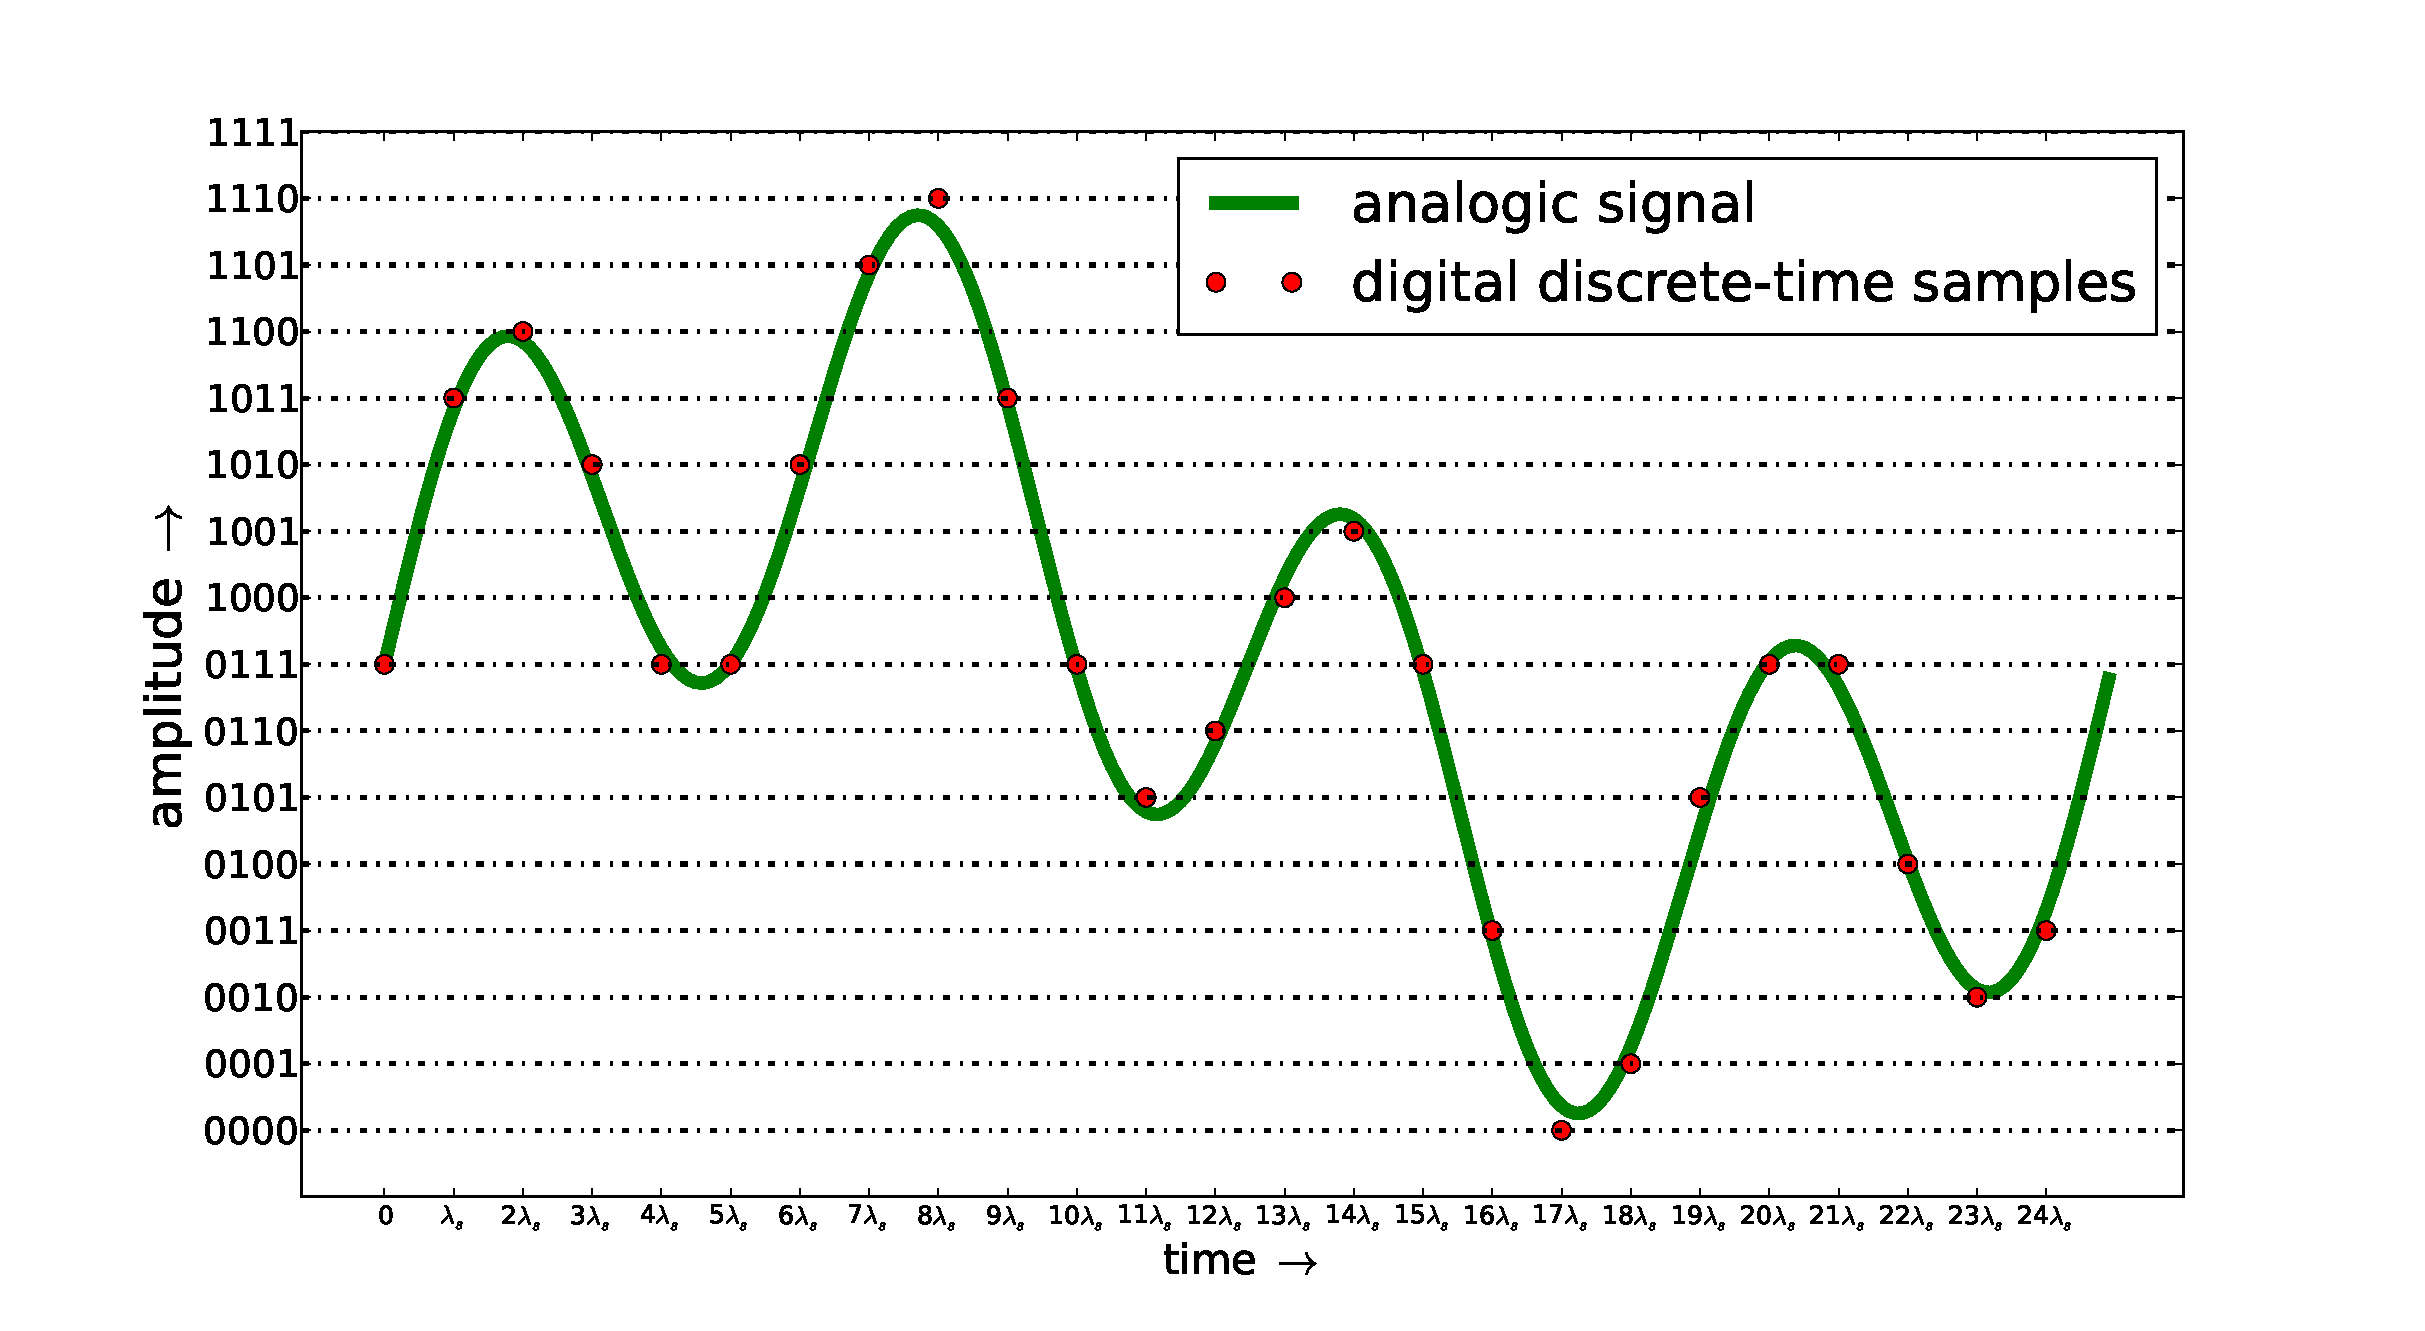
\includegraphics[width=\textwidth]{figures/pcm}
        \caption{Pulse Code Modulation (PCM) audio: an analogical signal is represented by 25 samples with 4 bits each.}
        \label{fig:PCM}
\end{figure*}

The Nyquist theorem~\cite{} states that the sampling frequency is twice the maximum frequency of the represented signal. Thus, for general musical purposes, it is necessary to have samples in a rate at least twice the highest frequency heard by humans, that is, $f_s \geq 2\times 20kHz = 40kHz$. This is the fundamental reason for the adoption of sampling frequencies like $44.1kHz$ and $48kHz$, standards in Compact Disks (CD) and broadcast systems (radio and television), respectively.

Within this framework, musical notes can be characterized. The note still stands paradigmatic as the 'fundamental unit' of musical structures and, in practice, it can unfold into sounds that uphold other approaches\footnote{Music from the twentieth century enlarged this traditional comprehension of music. This occurred in the concert music, specially in the concrete, electronic and electroacoustic styles. On the last decade of the century, it became evident that popular music had also incorporated sounds without defined pitch and temporal organization, to name a few of simple characteristics.}. 
Notes are also convenient for another reason: the average listener -- and considerable part of the specialists -- presupposes rhythmic and pitch organization (made explicit in section~\ref{sec:notasMusic}) as fundamental musical properties, and these are developed in traditional musical theory in terms of notes.

\subsection{Contributions and paper organization}

This article aims at representing musical structures and artifices by their discrete-time sonic characteristics. Results include mathematical relations, usually in terms of samples, and their direct computer program implementations. Despite the general interests involved, there are few books and computer implementations that tackle the subject. These mainly focus on computer implementations and ways to mimic traditional instruments, with scattered mathematical formalisms. A compilation of the works and their contributions is in the bibliography~\cite{dissertacao}. To the best of the author's knowledge, there is a lack of articles on the topic. Moreover, although current computer implementations use the analytical descriptions presented in this study in a implicit manner, it seems that there has been no concise and mathematical description of the processes implemented. 

In order to address this concise description of musical elements and structures, in terms of the digitilized sound, the objectives of this paper are:

\begin{enumerate}

\item Present a concise set of relations among musical basic elements and sequences of PCM audio samples. 

\item Introduce a framework of sound synthesis with control at sample level and with potential uses in psycho-acoustical experiments and high-fidelity synthesis.

\item Provide the accessibility of the developed framework. The analytic relations presented in this article are implemented as public domain scripts, i.e. small computer programs using accessible technologies for better distribution and validation. This constitute the \massa\ toolbox, available in an open Git repository~\cite{gitBook}. These scripts are written in Python and make use of external libraries, such as Numpy that performs calls to Fortran routines for better computational efficiency. Part of the scripts have been transcribed to JavaScript and native Python with readiness, what favors their use in Web browsers such as Firefox and Chromium~\cite{numpy, audiolab, tutpython, python}. Furthermore, these are all open technologies, that is, published using licenses that allow copy, distribution and use of any part for research and derivatives. This way, the work presented here is embedded in recommended practices for availability and eases co-authorship processes~\cite{Raymond,Lessig}.

\item To provide a didactic presentation of the content to favor its apprehension and usage. It is worthwhile to mention that this subject comprises diverse topics on signal processing, music, psycho-acoustics and programming.

\end{enumerate}

The remaining parts of this work are organized as follows: section~\ref{sec:discNote} characterizes the basic musical note; internals of the musical note is further developed in section~\ref{sec:internalVar}; section~\ref{sec:notesMusic} tackles the organization of musical notes in higher levels of musical structure~\cite{Wisnick,Webern,Lerdhal,Cook,Lacerda}. As these descriptions embody topics such as psycho-acoustics, cultural traditions, formalisms and protocols, the text points to external complements as needed~\cite{Zamacois,Schoenberg,microsound}.

The next section is a minimum text in which musical elements are presented side-by-side with the discrete-time samples they result. In order to account for validation and sharing, implementations on computer code of each one of these relations are gathered in the \massa\ toolbox together with little musical montage resulting from them.

%Representing musical structures and artifices by it's discrete sound characteristics is the purpose of this work. The results include mathematical relations and it's computer program implementations. Next section exposes the theoretical description, which is implemented as scripts in a one-to-one relation to the equations.

%\subsection{Sound and digital audio}

%Sound is a longitudinal wave of mechanical pressure. The frequency bandwidth between $20Hz$ and $20kHz$ is appreciated by human hearing system with boundaries dependent on the person, climate conditions and sonic characteristics itself~\cite{Roederer}. If considered the speed of sound of $\approx 343.2 m/s$, this limits corresponds to $\frac{343.2}{20} = 17.16\,m$ and $\frac{343.2}{20000}=17.16\,mm$.

%Human perception of sound involves captivation by bones, stomach, ears, transfer functions of head and processing torso and nervous system. Besides that, the ear is a dedicated organ to the capture of this waves. Its mechanism decomposes sound into its sinusoidal spectrum and delivers them to the nervous system. This sinusoidal components are crucial to musical phenomena, as one can observe in the composition of sounds with musical interest and in tunings and scales. Subsection~\ref{subsec:dicNote} exposes the presence of sinusoid in discrete-time audio and characterizes a basic musical note.

%The representation of sound is called audio (although these terms are often used without distinction), and this can be provenient from caption by microphones or from synthesis. Often enough, digital audio is specified by protocols that eases file storage and transferring, in cost of a direct representation or even some loss in quality. Standard representation of digital audio, on the other hand, consists of samples equally spaced by $\lambda_s$ durations in time, with each sample specified by a sample number of bits. This is called the Pulse Code Modulation representation of sound (PCM). A PCM digital sound is characterized by it's sampling frequency $f_s=\frac{1}{\lambda_s}$, also called sampling rate, and bit depth, which is the number of bits used of representing the amplitude of each sample. Figure~\ref{fig:PCM} shows $25$ samples of a PCM audio with $4$ bits each. The $2^4=16$ possible steps for each sample, together with the regular spacing $\lambda_s$ between them, introduces a quantization error. This noise, caused by this errors, diminishes as these spacing diminishes.


%\begin{figure*}
%    \centering
%        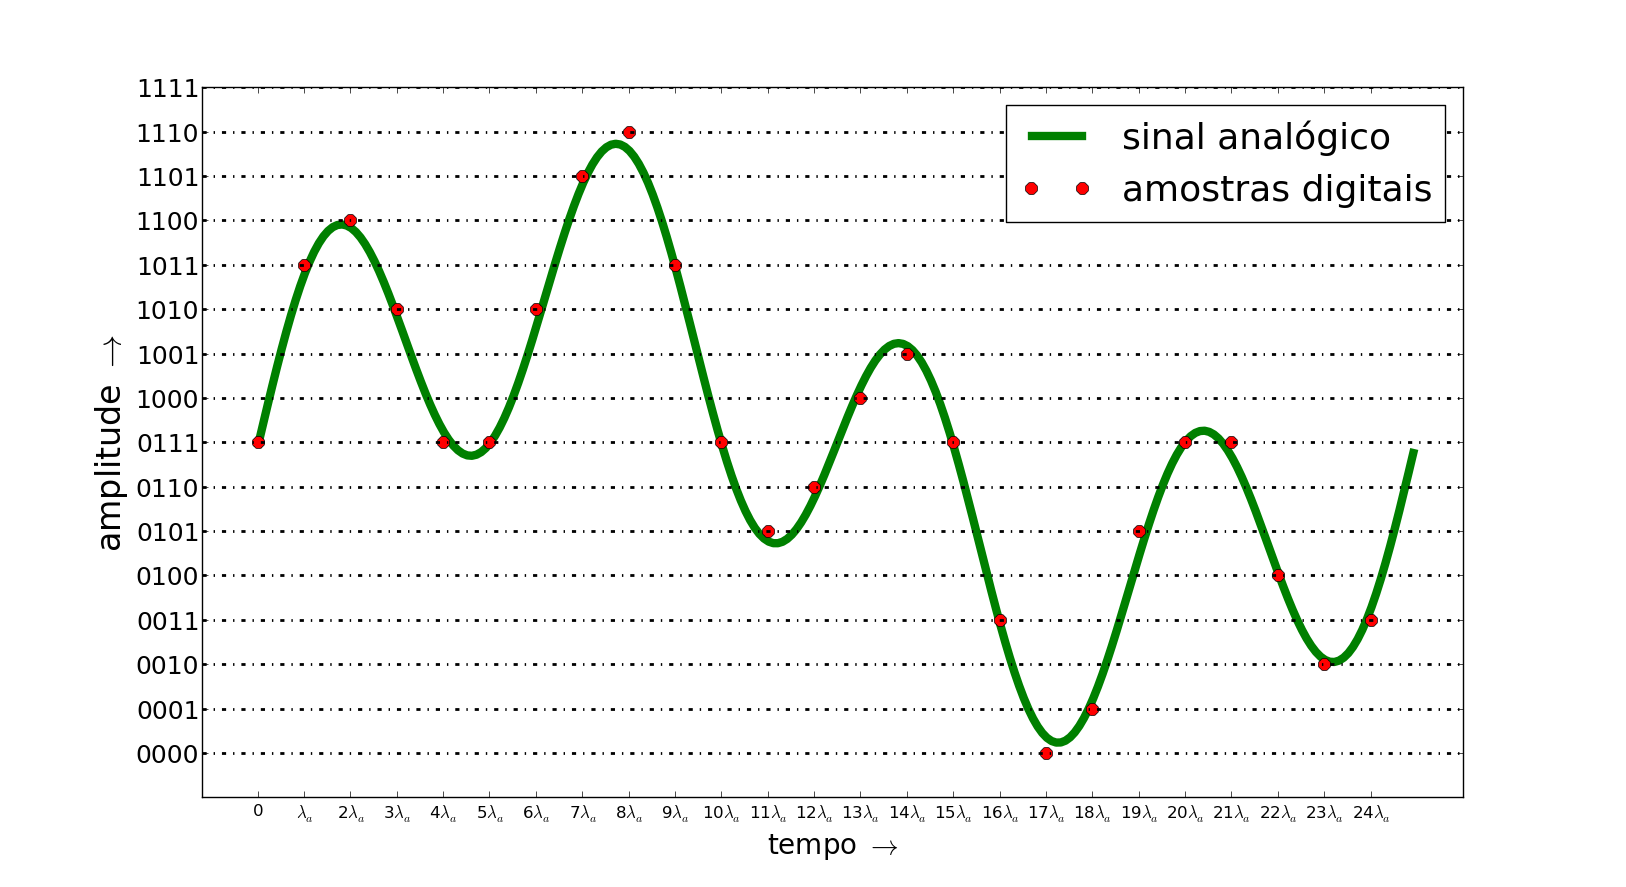
\includegraphics[width=\textwidth]{pcm}
%        \caption{Pulse Code Modulation (PCM) audio: an analogical signal is %represented by 25 samples with 4 bits each.}
%        \label{fig:PCM}
%\end{figure*}




%By the Nyquist theorem, it is known that half the sampling frequency is the maximum frequency of the signal. Thus, it is necessary to have a sampling frequency at least twice the highest frequency heard by humans $f_s \geq 2\times 20kHz = 40kHz$. This is the basis for the use of the sampling frequencies $44.1kHz$ and $48kHz$, standards in Compact Disks (CD) and Broadcast systems (Radio and TV), respectively.

%\subsection{Sonic art and musical theory}

%A common definition for music is the art made by sounds and silences. For the average listener -- and a reasonable part of specialists -- the notion of music presupposes rhythmic and pitch organization such as explained in subsection~\ref{subsec:notesMusic}. Music from the twentieth century enlarged this traditional comprehension of music. This occurred in concert music, specially in the concrete, electronic and electroacoustic styles. On the last decade of the century, it was evident that popular music has also incorporated sounds without defined pitch and temporal organization out of simple metrics. Even though, the note stands paradigmatic as a 'fundamental unit' of musical structures and, in practice, it can unfold in sounds that observe this recent developments. The definition and expansion of the musical note as the fundamental unit of music is approached in subsections~\ref{subsec:discNote} and~\ref{subsec:internalVar}, respectively. Subsection~\ref{subsec:notesMusic} tackles the organization of musical notes in a higher level~\cite{Wisnick,Webern,Lerdhal,Cook,Lacerda}.

%Musical theory embody topics as diverse as psycho-acoustics, cultural manifestations and formalisms. The section~\ref{sec:results} point this topics as needed and designate external complements~\cite{Zamacois,Schoenberg,microsound}.

%\subsection{Computational implementation}

%The results presented in this article are implemented as scripts, i.e.\ small computer programs implemented using accessible technologies for better distribution and validation. This constitute the \massa\ toolbox, available in public domain in an open Git repository~\cite{gitBook}. This scripts are written in Python and make use of external libraries Numpy and Scikits/Audiolab that performs calls to Fortran routines for better computational efficiency. Part of this code has been transcribed to JavaScript and native Python with readiness, what points to uses of this contribution in Web browsers such as Firefox and Chromium~\cite{numpy, audiolab, tutpython, python}.

%This are all open technologies, that is, published using licenses that allows copy, distribution and use of any part for research and derivatives. This way, the work here presented is available and eases co-authorship processes~\cite{Raymond,Lessig}. 

%\subsection{Objectives}
%\label{subsec:objectives}
%The main goal of this article is to present a concise set of relations among musical basic elements and sequences of PCM audio samples. The next section is a minimum text in which music elements are presented side-by-side with the discrete-time samples they result. As validation and sharing, implementations on computer code of these relations and little musical pieces where gathered the \massa\ toolbox, available online.

%Secondary objectives include presenting a framework of sound synthesis with control at sample level, with potential uses in psychoacoustical experiments and high-fidelity synthesis. The didactic presentation of the content favors use and apprehension on a problem which calls diverse topics to be tackled: signal processing, music and psycho-acoustics, to name just a few.

%\subsection{Related work}
%Due to the general interest, and number of knowledge areas involved, there is a number of books and computer implementations that are of interest or present similarities to what is presented in this work. A more detailed comparison of them is pointed out in the bibliography~\cite{dissertacao}. There is almost no articles which could be found on the topic. In summary, there are computer implementations that use this analytical descriptions implicitly, but there is no such a concise and mathematical description of the processes implemented, as they aim to be libraries for sound and music. There are books on the topic that cover various aspects of effects and physical modeling, but none of them carry a concise description of musical elements and structures, but focus on aspects of musical sounds and ways to mimic traditional instruments.


\section{Characterization of the discrete-time musical note} \label{sec:discNote}

In diverse artistic and theoretical contexts, music is conceived as constituted by fundamental units called notes, ``atoms'' that constitute music itself~\cite{Wisnick, Lovelock, Webern}.
Nowadays, these notes are understood as central elements of certain musical paradigms. In a cognitive perspective, the notes are seen as discretized elements that easy and enrich the flow of information through music~\cite{Roederer, Lacerda}.
Canonically, the principal properties of a musical note are duration, volume, pitch and timbre~\cite{Lacerda}. These qualities can be managed quantitatively, dictated by the evenly time spaced sonic samples.

All the relations described in this section are implemented at the file \emph{eqs2.1.py} of the \massa\ toolbox. Musical pieces \emph{5 sonic portraits} and \emph{reduced-fi} are also available online in order to corroborate the concepts.

\subsection{Duration}

The sample frequency $f_s$ is defined as the number of samples in each second of the discrete-time signal. Let $T_i=\{t_i\}$ be an ordered set of real samples separated by $\delta_s=1/f_s$ seconds. A musical note of duration $\Delta$ seconds is presented as a sequence $T_i^{\Delta}$ of $\lfloor \Delta . f_s \rfloor $ samples. That is, the integer part of the multiplication is considered, and an error of at most $\delta_s$ missing seconds is admitted, which is usually fine for musical purposes. As an example, if $f_s=44.1kHz \;\;\Rightarrow\;\;\lambda_s=\frac{1}{44100}\approx 23$ microseconds. Thus:


\begin{equation}\label{eq:dur}
T_{i}^{\Delta}={\{t_i\}}_{i=0}^{\lfloor \Delta . f_s \rfloor -1}
\end{equation}

With $\Lambda=\lfloor \Delta . f_a \rfloor$, the number of samples in the sequence, the more condensed notation is $T_i^\Delta=\{t_i\}_0^{\Lambda-1}$.

\subsection{Volume}\label{subsec:volume}

The sensation of sound volume depends on reverberation and harmonic distribution, among other characteristics described on section~\ref{sec:varInternas}. One can get volume variations through the potency of the wave~\cite{Chowning}:

\begin{equation}\label{eq:potencia}
pot(T_i)=\frac{\sum_{i=0}^{\Lambda -1} t_i^2}{\Lambda}
\end{equation} 

The final volume is dependent on the speakers amplification of the signal. Thus, what matters is the relative potency of a note in relation to the other ones around it, or the potency of a music section in relation to the rest. Differences in volume are measured in decibels, calculated directly from the amplitudes through energy or potency:

\begin{equation}\label{decibels}
V_{dB}=10log_{10}\frac{pot(T^{'}_i)}{pot(T_i)}
\end{equation}

The quantity $V_{dB}$ has the decibel unit ($dB$). 
For each $10dB$ it is associated a ``doubled volume''.
A handy reference is $10dB$ for each step in the intensity scale: \emph{pianissimo}, \emph{piano}, \emph{mezzoforte}, \emph{forte} e \emph{fortissimo}. Other useful references are $dB$ values related to double amplitude or potency:

\begin{equation}\label{eq:ampVol}
\begin{split}
t_i^{'}=2 . t_i \Rightarrow pot(T^{'}_i)=4 . pot(T_i) \Rightarrow \\ \Rightarrow V^{'}_{dB}=10log_{10} 4 \approx 6 dB
\end{split}
\end{equation}

\begin{equation}\label{eq:potVol}
\begin{split}
pot(T^{'}_i)=2 pot(T_i) \Rightarrow \\ \Rightarrow V^{'}_{dB}=10log_{10} 2 \approx 3 dB
\end{split}
\end{equation}

and the amplitude gain for a sequence whose volume has been doubled ($10dB$):

\begin{equation}\label{eq:dobraVol}
\begin{split}
10log_{10}\frac{pot(T^{'}_i)}{pot(T_i)} = 10 \quad \Rightarrow \\ \Rightarrow \quad \sum_{i=0}^{\lfloor \Delta.f_a \rfloor -1}t^{'2}_i=10\sum_{i=0}^{\Lambda-1}t_i^2=\sum_{i=0}^{\Lambda-1}(\sqrt{10}.t_i)^2 \\
\therefore \quad t^{'}_i=\sqrt{10}t_i \quad \Rightarrow \quad t^{'}_i \approx 3.16t_i
\end{split}
\end{equation}

As shown, it is necessary an amplitude increase by a bit more than a factor of 3 for a doubled volume. These values are guides for increasing or decreasing the absolute values on the sample sequences with musical purposes. The conversion from decibels to amplitude gain (or attenuation) is straightforward:

\begin{equation}\label{ampDec}
A = 10^{\frac{V_{dB}}{20}}
\end{equation}

where $A$ is the multiplicative factor that relates the amplitudes before and after the amplification.

\subsection{Pitch}

As exposed in the previous subsections, to a note corresponds a sequence $T_i$ in which duration and volume are directly related to the size of the sequence and the amplitude of its samples, respectively. The pitch is specified by the fundamental frequency $f_0$ whose cycle has duration $\delta_{f_0}=1/f_0$. This duration, multiplied by the sampling frequency $f_s$ results on the number of samples per cycle: $\lambda_{f_0}=f_s . \delta_{f_0} =f_a/f_0$.

For didactic reasons, be $f_0$ such that it divides $f_s$ and $\lambda_{f_0}$ results integer. If $T_i^f$ is a sonic sequence of fundamental frequency $f$, then:

\begin{equation}\label{periodicidade}
     T^f_i=\left\{ t_i^f \right\}=\left\{ t^f_{i+\lambda_{f}}  \right\}= \left\{ t^f_{i+\frac{f_a}{f}} \right\}
\end{equation}

In the next section, frequencies $f$ that does not divide $f_s$ will be considered. This restriction does not imply in lost of generality of this section's content.

\subsection{Timbre}

In a sound with harmonic spectrum, the (wave) period corresponds to the duration of the cycle, given by the inverse of the fundamental frequency. The trajectory of the wave inside the period - called the waveform - defines a harmonic spectrum and, thus, a timbre\footnote{Timbre is a subjective and complex characteristic. Physically, the timbre is multidimensional and given by the temporal dynamics of energy in the spectral components that are harmonic or noisy. Beyond that, the word timbre is used to designate different things: one same note has different timbres, a same instrument has different timbres, two instruments of the same family have, at the same time, the same timbre that blends them in the same family, and different timbres as they are different instruments. It is worth to mention that timbre is not always manifested in spectral traces, since cultural or circumstantial aspects alter our perception of timbre}. Musically, it matters that sonic spectra with minimum differences can result in timbres with crucial expressive differences and, consequently, different timbres can be produced by using different spectra\cite{Roederer}.

The simplest case is the spectrum that consists of only of the fundamental frequency $f$. This defines the sinusoid: a frequency in pure oscillatory movement called `simple harmonic movement'. Be $S_i^f$ a sequence whose samples $s_i^f$ describes a sinusoid of frequency $f$:

\begin{equation}\label{sinusoid}
     S^f_i=\{ s^f_i \}=\Bigl\{ \sin\bigl(2\pi \frac{i}{\lambda_f} \bigr)  \Bigr\} = \Bigl\{ \sin\bigl(2\pi f \frac{i}{f_s}\bigr)  \Bigr\} 
\end{equation}

where $\lambda_f=\frac{f_s}{f}=\frac{\delta_f}{\lambda_s}$  is the number of samples in the period.

In a similar fashion, other waveforms are applied in music for their spectral qualities and simplicity. While the sinusoid is an isolated point in the spectrum, these waves present a succession of harmonic components. These waveforms are specified in equations~\ref{sinusoid},~\ref{sawTooth},~\ref{triangular} and~\ref{square} and illustrated in Figure~\ref{fig:formasDeOnda}.
These artificial waveforms are traditionally used in music for synthesis and oscillatory control of variables. They are also useful outside musical contexts\cite{Openheim}.

The sawtooth presents all components of the harmonic series with decreasing energy of $-6dB/octave$. The sequence of temporal samples can be described as:

\begin{equation}\label{sawTooth}
     D^f_i=\left\{ d^f_i \right\}=\left\{ 2\frac{i\,\%\lambda_f}{\lambda_f} -1 \right\}
\end{equation}

The triangular waveform present only odd harmonics falling with $-12dB/octave$:
\begin{equation}\label{triangular}
     T^f_i=\left\{ t^f_i \right\}=\left\{1- \left| 2 - 4\frac{i\,\%\lambda_f}{\lambda_f} \right| \right\}
\end{equation}

The square wave preservers only odd harmonics falling at $-6dB/octave$:

\begin{equation}\label{square}
     Q^f_i=\left\{ q^f_i \right\}= \left\{
         \begin{array}{l l}
              1 & \quad \text{for } \; \; (i\,\%\lambda_f)   <  \lambda_f /2  \\
              -1 & \quad \text{otherwise}\\
         \end{array} \right.
\end{equation}


The square wave can be used in a subtractive synthesis with the purposes of mimicking a clarinet. This instrument has only the odd harmonic components and the square wave is convenient with its abundant energy in high frequencies.
The sawtooth is a common starting point for a subtractive synthesis, because it has both odd and even harmonics with high energy. In general, these waveforms are appreciated as excessively rich in sharp harmonics, and attenuator filtering on treble and middle parts of the spectrum is specially useful for reaching a more natural and pleasant sound. 
The relatively attenuated harmonics of the triangle wave makes it the more functional - among the listed ones - to be used in the synthesis of musical notes without any treatment. The sinusoid is often a nice choice, but a problematic one. While pleasant if not loud in a very high pitch (above 500Hz, it requires careful dosage), the pitch is not accuratly detected, specially in low frequencies. It requires a big amplitude to give sinusoid volume, if compared to other waveforms. Both particularities are seen as a consequence of the non-existence of pure sinusoidal sounds in nature~\ref{roederer}.


\begin{figure*}
    \centering
        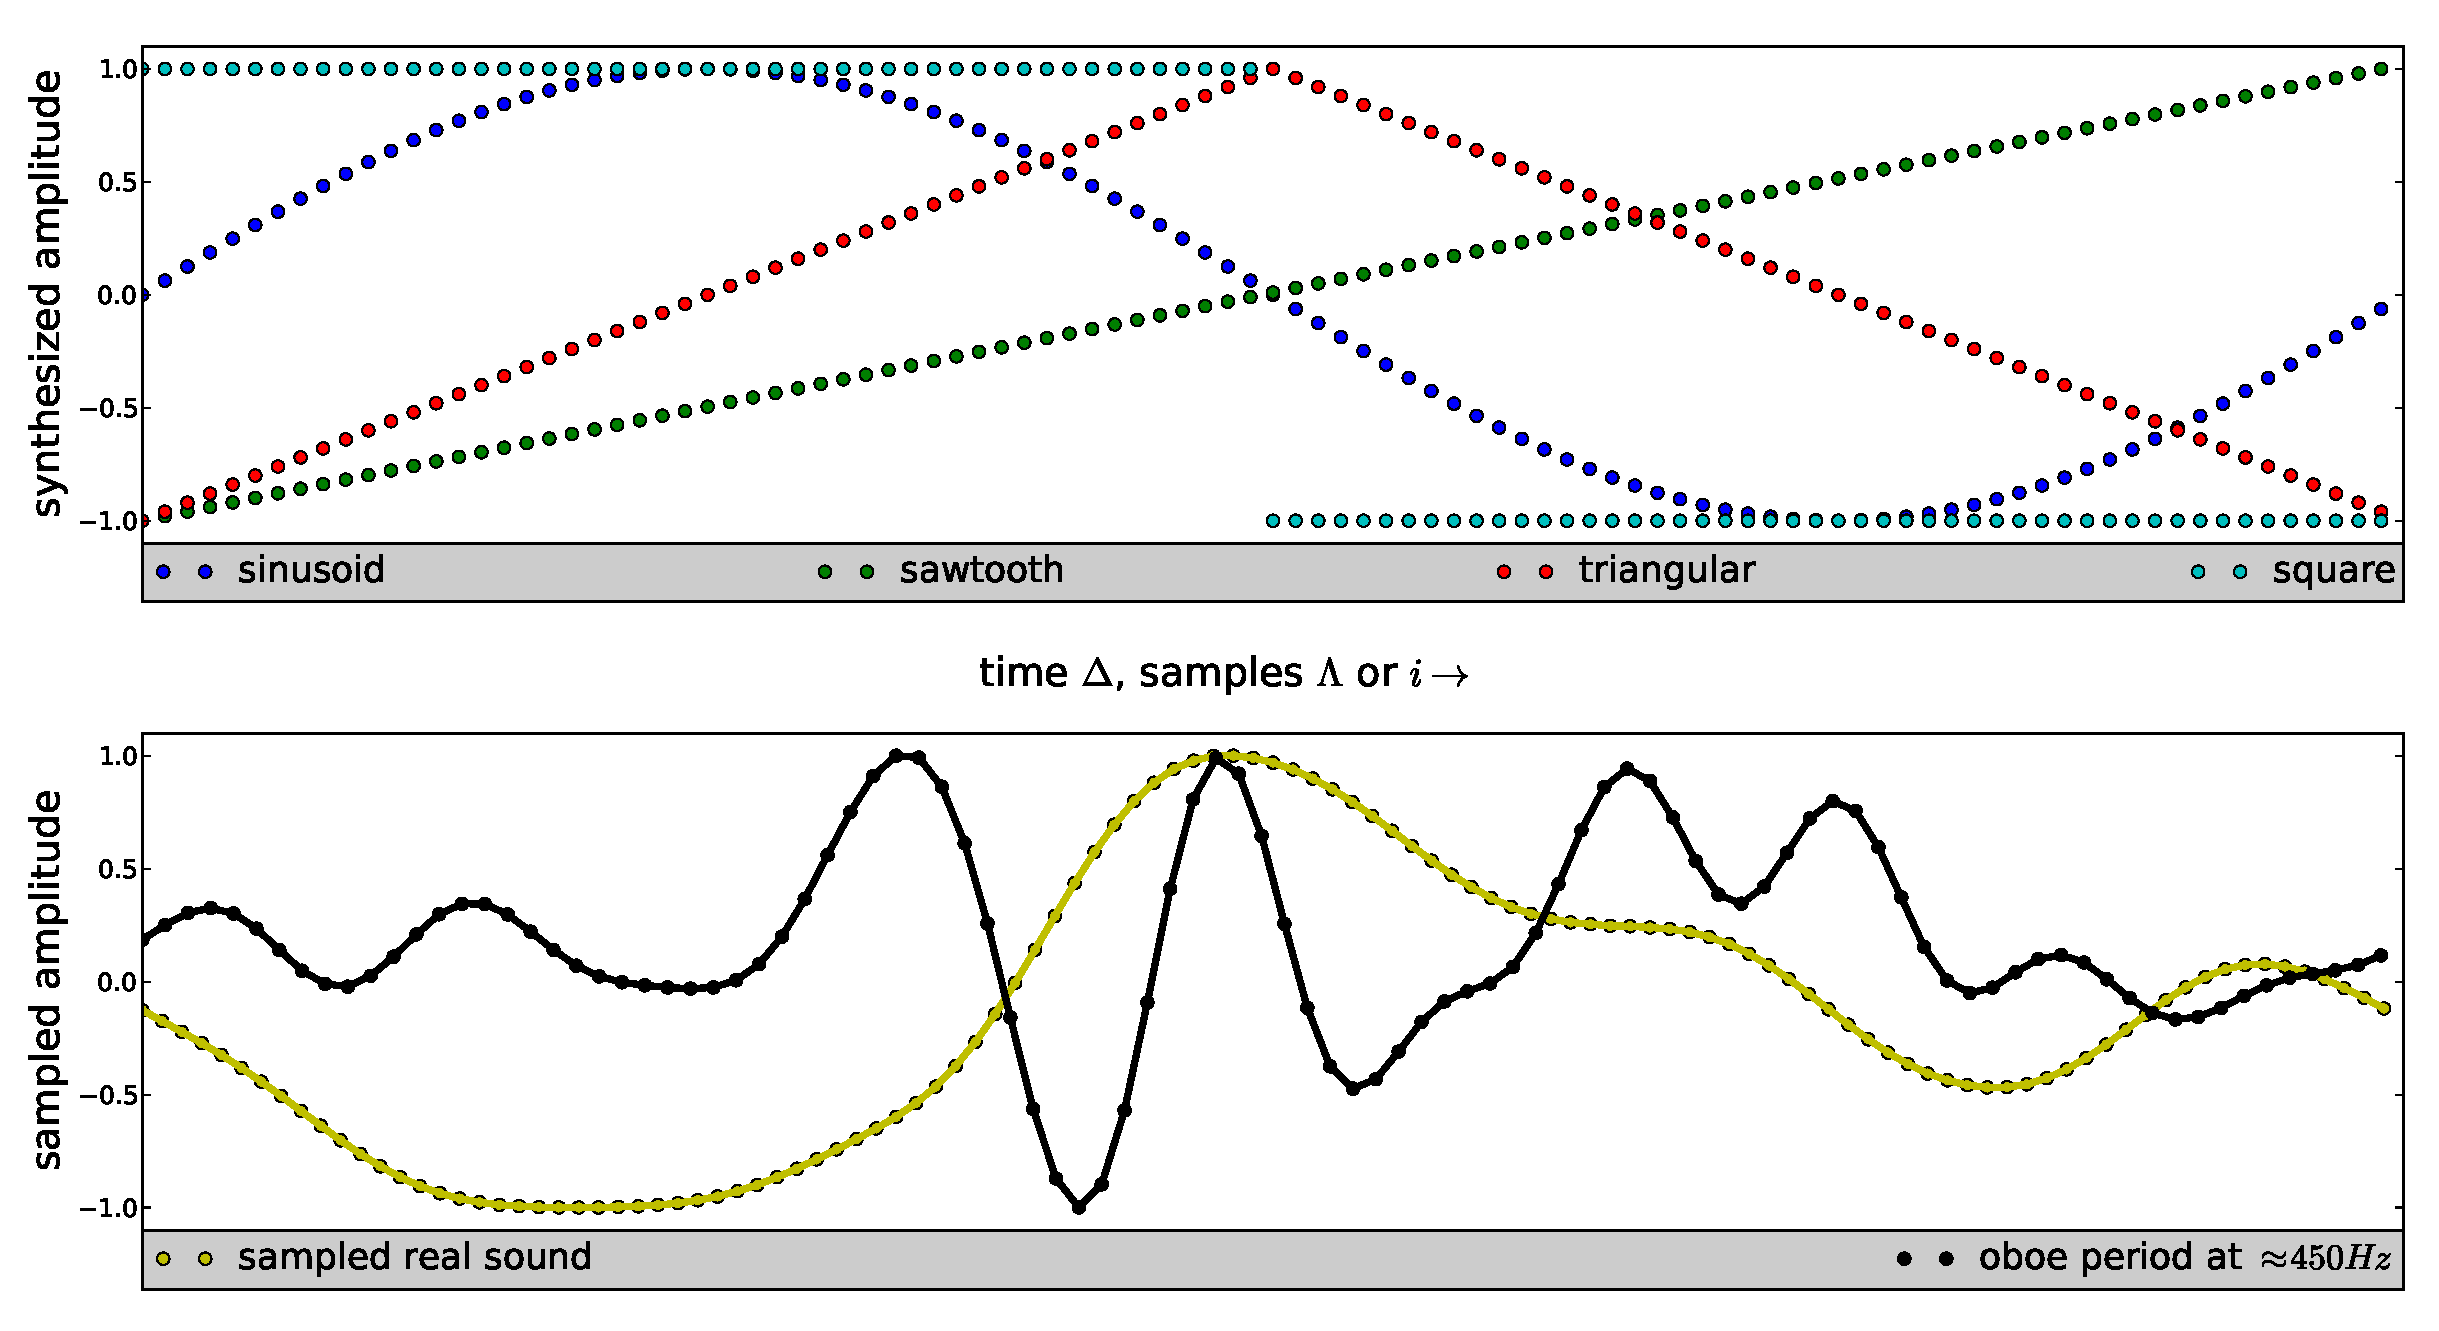
\includegraphics[width=\textwidth]{figures/waveForms_}
    \caption{Basic musical waveforms: (a) the synthetic  waveforms; (b) the real waveforms.}
        \label{fig:formasDeOnda}
\end{figure*}

Figure~\ref{fig:formasDeOnda} presents the waveforms described in equations  ~\ref{senoide}, ~\ref{denteDeSerra}, ~\ref{triangular} and ~\ref{quadrada} for $\lambda_f=100$ (period of $100$ samples). If $f_s=44.1kHz$, the PCM standard in Compact Disks, the wave has fundamental frequency $f=\frac{f_a}{\lambda_f}=\frac{44100}{100} = 441 \; Herz$, around A4, just above the central "C", whatever the waveform is.

The spectrum of each basic waveform is in Figure~\ref{fig:espectroDeOndas}. The isolated and exactly harmonic components of the spectrum is a consequence of the fixed period usage. The sinusoid consists of an one and only node in the spectrum, pure frequency. The figure exibit the spectra described: the sawtooth is the only waveform with a complete harmonic series (odd and even components); triangular and square waves has the same components (odd harmonics), decaying at $-12dB/octave$ and $-6dB/octave$, respectively.

\begin{figure*}
    \centering
        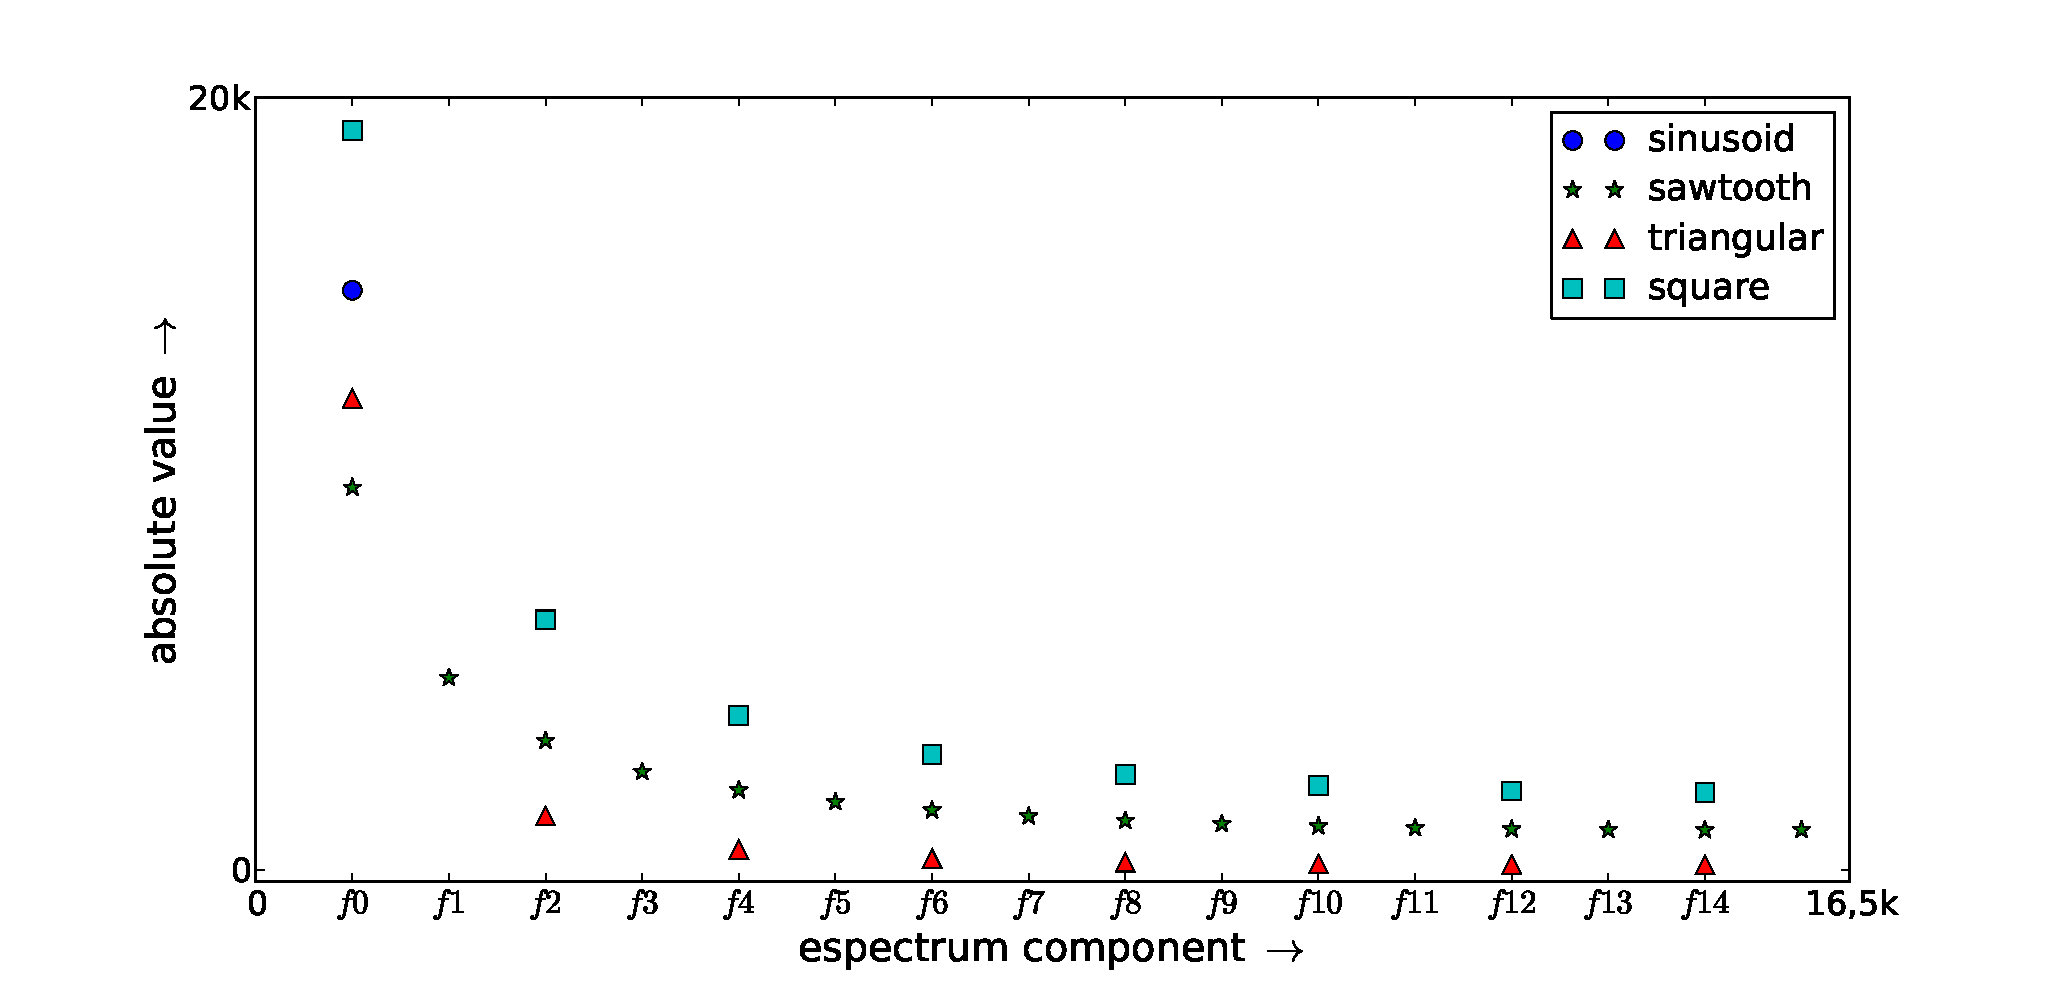
\includegraphics[width=\columnwidth]{figures/waveSpectrum}
    \caption{Spectrum of basic artificial musical waveforms.}
        \label{fig:espectroDeOndas}
\end{figure*}

The harmonic spectrum is composed of frequencies $f_n$ that are multiples of the fundamental frequency: $f_n=(n+1)f_0$. As the human linear perception of pitch follows  a geometric progression of frequencies, the spectrum has notes different from the fundamental frequency (see equation~\ref{eq:serieHarmonica}). Additionally, the number of harmonics will be limited by the Nyquist frequency $f_s/2$.

From a musical perspective, it is critical to internalize that energy in a component of frequency $f_n$ means an oscillation in the constitution of the sound, purely harmonic and in that frequency $f_n$. This energy, specifically concentrated on the frequency $f_n$, is separated by the ear for further cognitive processes (this separation is done in many species with mechanisms similar to the human cochlea~\cite{Roederer}).

The sinusoidal components are usually the main responsibles for timbre qualities. If they are not presented in harmonic proportions (small number relations), the sound is perceived as noisy or dissonant, in opposition to sonorities with an unequivocally established fundamental. Furthermore, the notion of absolute pitch relies on the similarity of the spectrum to the harmonic series~\cite{Roederer}. 

In the case of a fixed length period and waveform, the spectrum is perfectly harmonic and static and  each waveform is compound of specific proportions of harmonic components. High  curvatures are sign of high harmonics in the wave. Figure~\ref{fig:formasDeOnda} depicts a wave, labeled as ``sampled real sound'', with a period of $\Lambda_f=114$ samples, extracted from a relatively well behaved recorded sound. The oboe wave was also sampled in $44.1kHz$. The chosen period for sampling was relatively short, with $98$ samples, and corresponds to the frequency $\frac{44100}{98}=450Hz$, which corresponds to a slightly out-of-tune A4 pitch. One can notice from the curvatures: the oboe's rich spectrum in high frequencies and the lower spectrum of the real sound.

The sequence 
$ R_i=\{ r_i \}_0^{\lambda_f-1}$ of samples in the real sound of Figure~\ref{fig:formasDeOnda} can be taken as basis for a sound $T_i^f$ in the following way: 

\begin{equation}\label{sampleandoFormaDeOnda}
     T^f_i=\{ t_i^f \}=\Bigl\{ r_{(i\,\%\lambda_{f})} \Bigr\}
\end{equation}

The resulting sound has the momentary spectrum of the original waveform. As a consequence of its repetition in an identical form, the spectrum is perfectly harmonic, without noise and with variations typical of the natural phenomenon. This can be observed in Figure~\ref{fig:espectroOboe}, that shows the spectrum of the original oboe note and a note with same duration and whose samples consists of the repetition of cycle of Figure~\ref{fig:formasDeOnda}. Summing up, the natural spectrum exhibits variations in the frequencies of the harmonics, in their intensities and some noise, while the note made from the sampled period has a perfectly harmonic spectrum.

\begin{figure*}
    \centering
        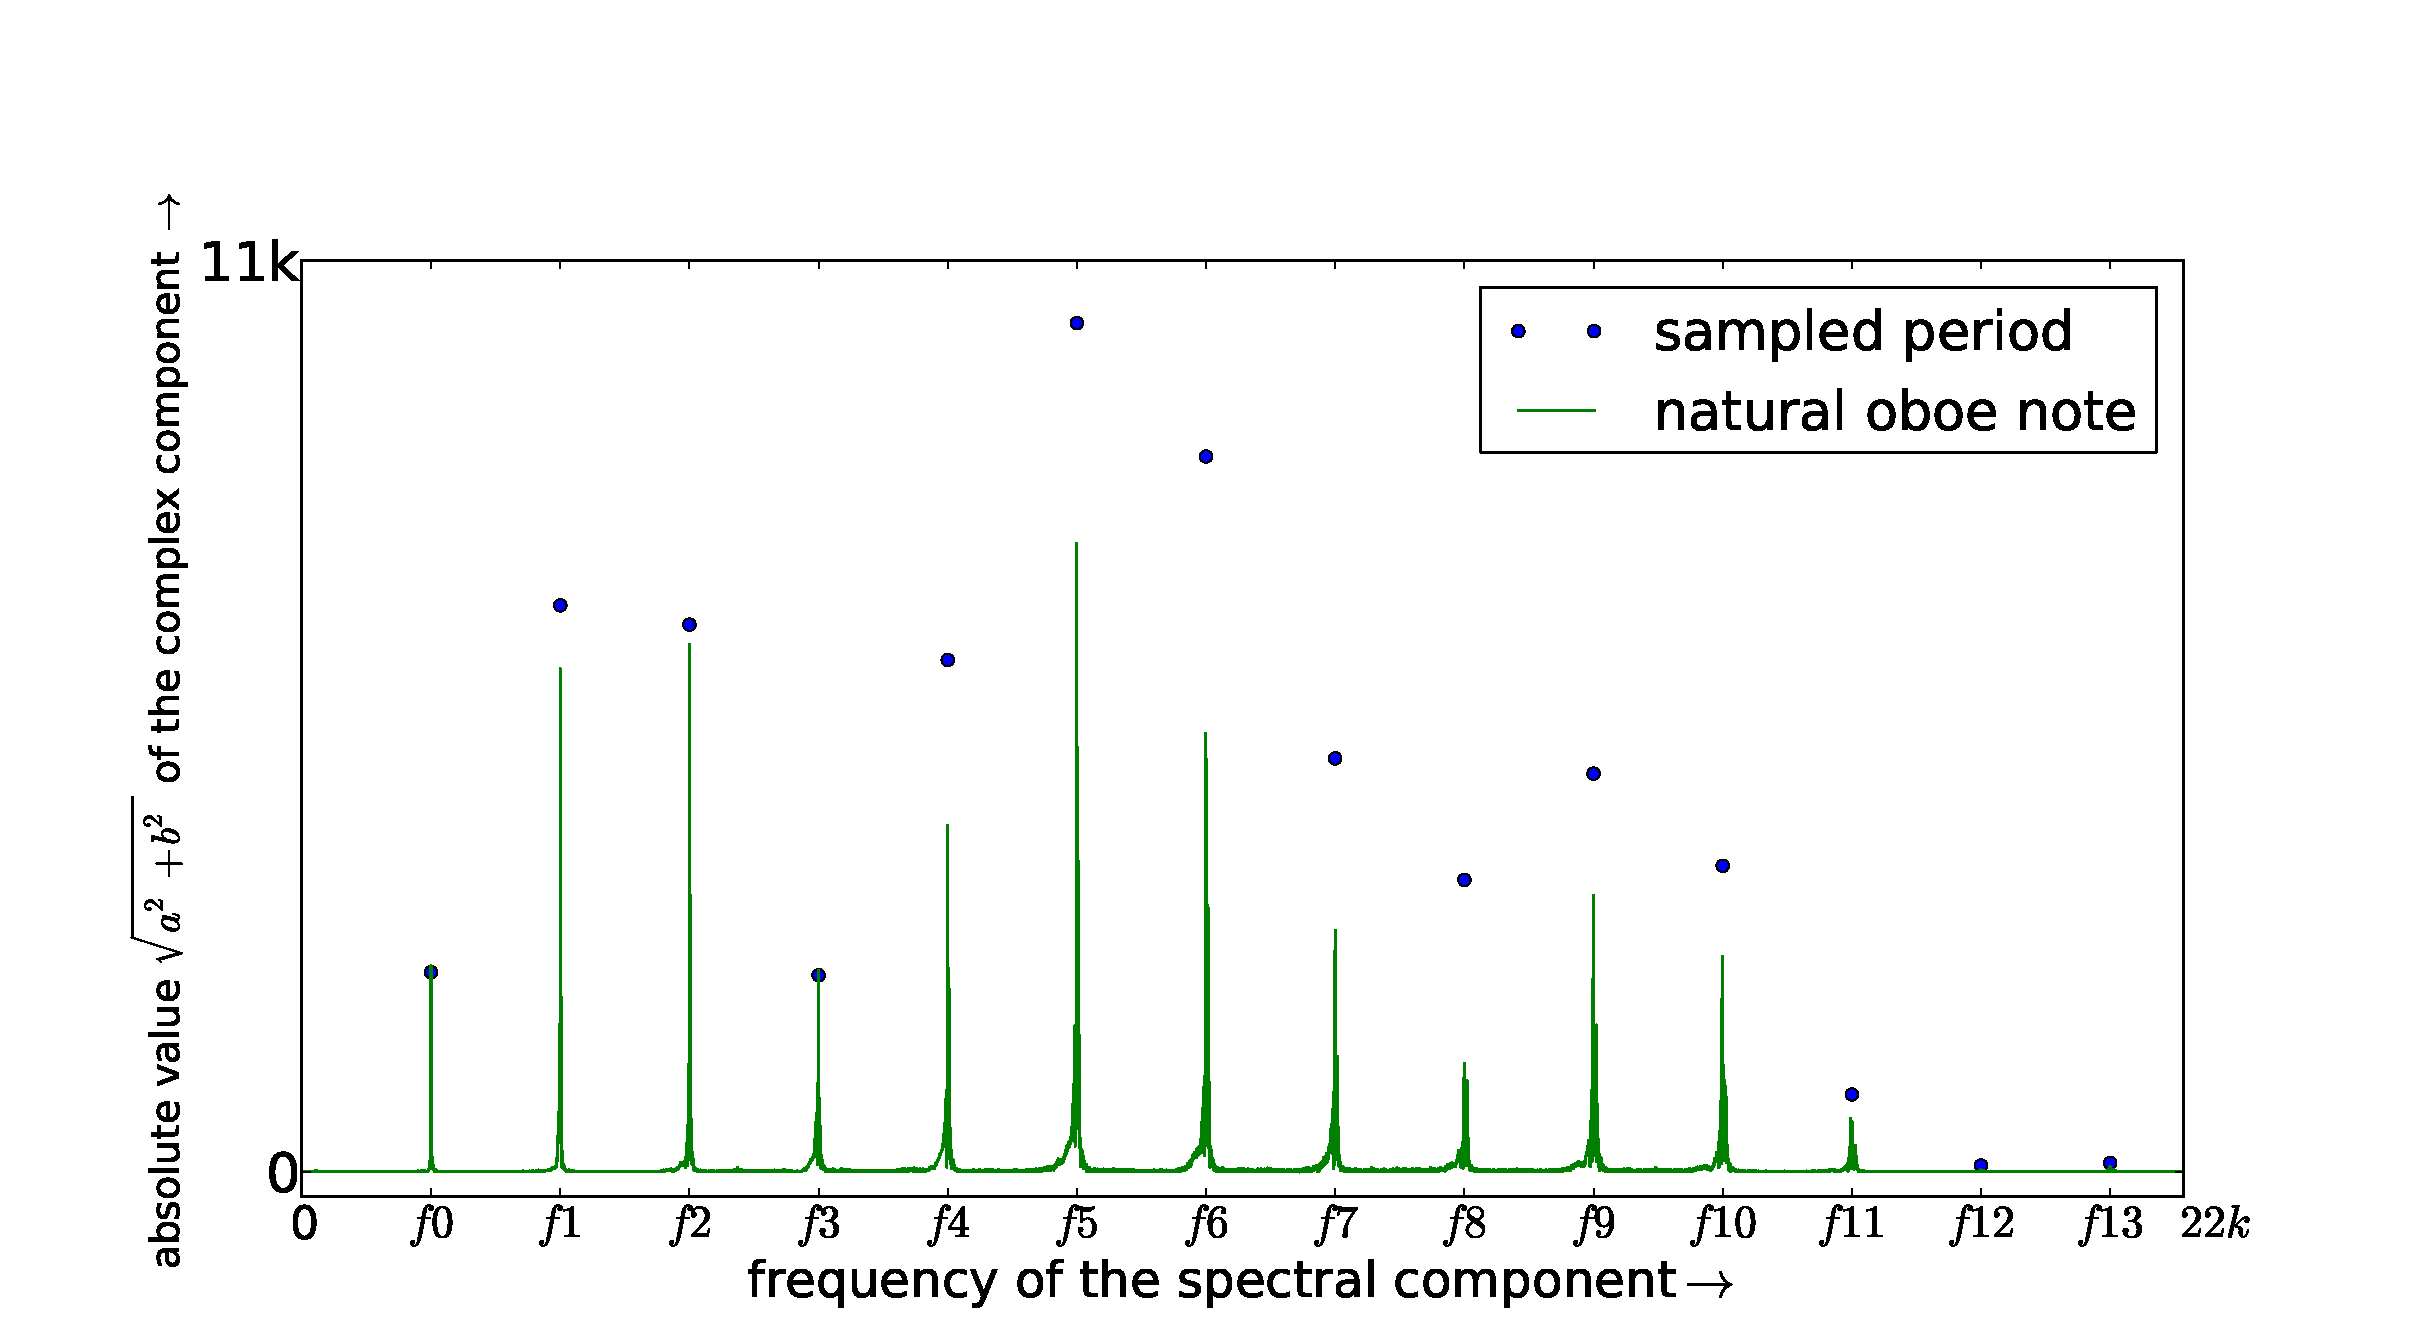
\includegraphics[width=\columnwidth]{figures/oboeNaturalSampledSpectrum}
    \caption{Spectrum of the sonic waves of a natural oboe note and from a sampled period. The natural sound has fluctuations in the harmonics and in its noise, while the sampled period note has a perfectly harmonic spectrum.}
        \label{fig:espectroOboe}
\end{figure*}

%%%%%%%%%%%%%%%%%%%%%%%%%%%%%%%%%%%%%%%%%%%%%%%%%%%%%%

\subsection{Spectrum at sampled sound}

The presence and behavior of these sinusoidal components in the discretized sound have some particularities. Considering a signal $T_i$ and its corresponding Fourier decomposition $\mathcal{F}\langle T_i\rangle=C_i=\{c_i\}_0^{\Lambda-1}$, the recomposition is the sum of the frequency components as time samples\footnote{It is important to note that the factor $\frac{1}{\Lambda}$ could be distributed among the Fourier transform and its reconstruction, as preferred.}:

\begin{equation}\label{recomposicaoFourier}
\begin{split}
t_i = & \frac{1}{\Lambda}\sum_{k=0}^{\Lambda-1}c_ke^{j \frac{2\pi k}{\Lambda} i } \\ 
    = & \frac{1}{\Lambda}\sum_{k=0}^{\Lambda-1}(a_k+ j . b_k)\left[cos(w_k i)   +j . sen(w_k i)\right]
\end{split}
\end{equation}

where $c_k = a_k + j . b_k$ defines the amplitude and phase of each frequency: $w_k=\frac{2\pi}{\Lambda}k$ in radians or $f_k=w_k\frac{f_a}{2\pi}=\frac{f_a}{\Lambda}k$ in Hertz, taking into account the respective limits in $\pi$ and in $\frac{f_a}{2}$ given by the Nyquist Theorem. As can be inferred, $j$ is the complex number, with $j^2=-1$.

For a sound signal, samples $t_i$ are real and are given by the real part of equation~\ref{recomposicaoFourier}:

\begin{equation}\label{moduloEfase}
\begin{split}
t_i& = \frac{1}{\Lambda}\sum_{k=0}^{\Lambda-1}\left[a_k cos(w_k i) -b_k sen(w_k i)\right] \\
   & = \frac{1}{\Lambda}\sum_{k=0}^{\Lambda-1}\sqrt{a_k^2 + b_k^2} \; cos\left[w_k i - tg^{-1}\left(\frac{b_k}{a_k}\right)\right]
\end{split}
\end{equation}

Equation~\ref{moduloEfase} shows how the imaginary term of $c_k$ adds a phase to the real sinusoid: the terms $b_k$ enables the phase sweep $\left[-\frac{\pi}{2},+\frac{\pi}{2}\right]$ given by $tg^{-1}\left(\frac{b_k}{a_k}\right)$ which has this image. The terms $a_k$ specifies the right or left side of the trigonometric circle, which completes the phase domain: $\left[-\frac{\pi}{2},+\frac{\pi}{2}\right] \cup \left[\frac{\pi}{2},\frac{3\pi}{2}\right]\equiv [2\pi]$.



 \begin{figure}[h!]
     \centering
         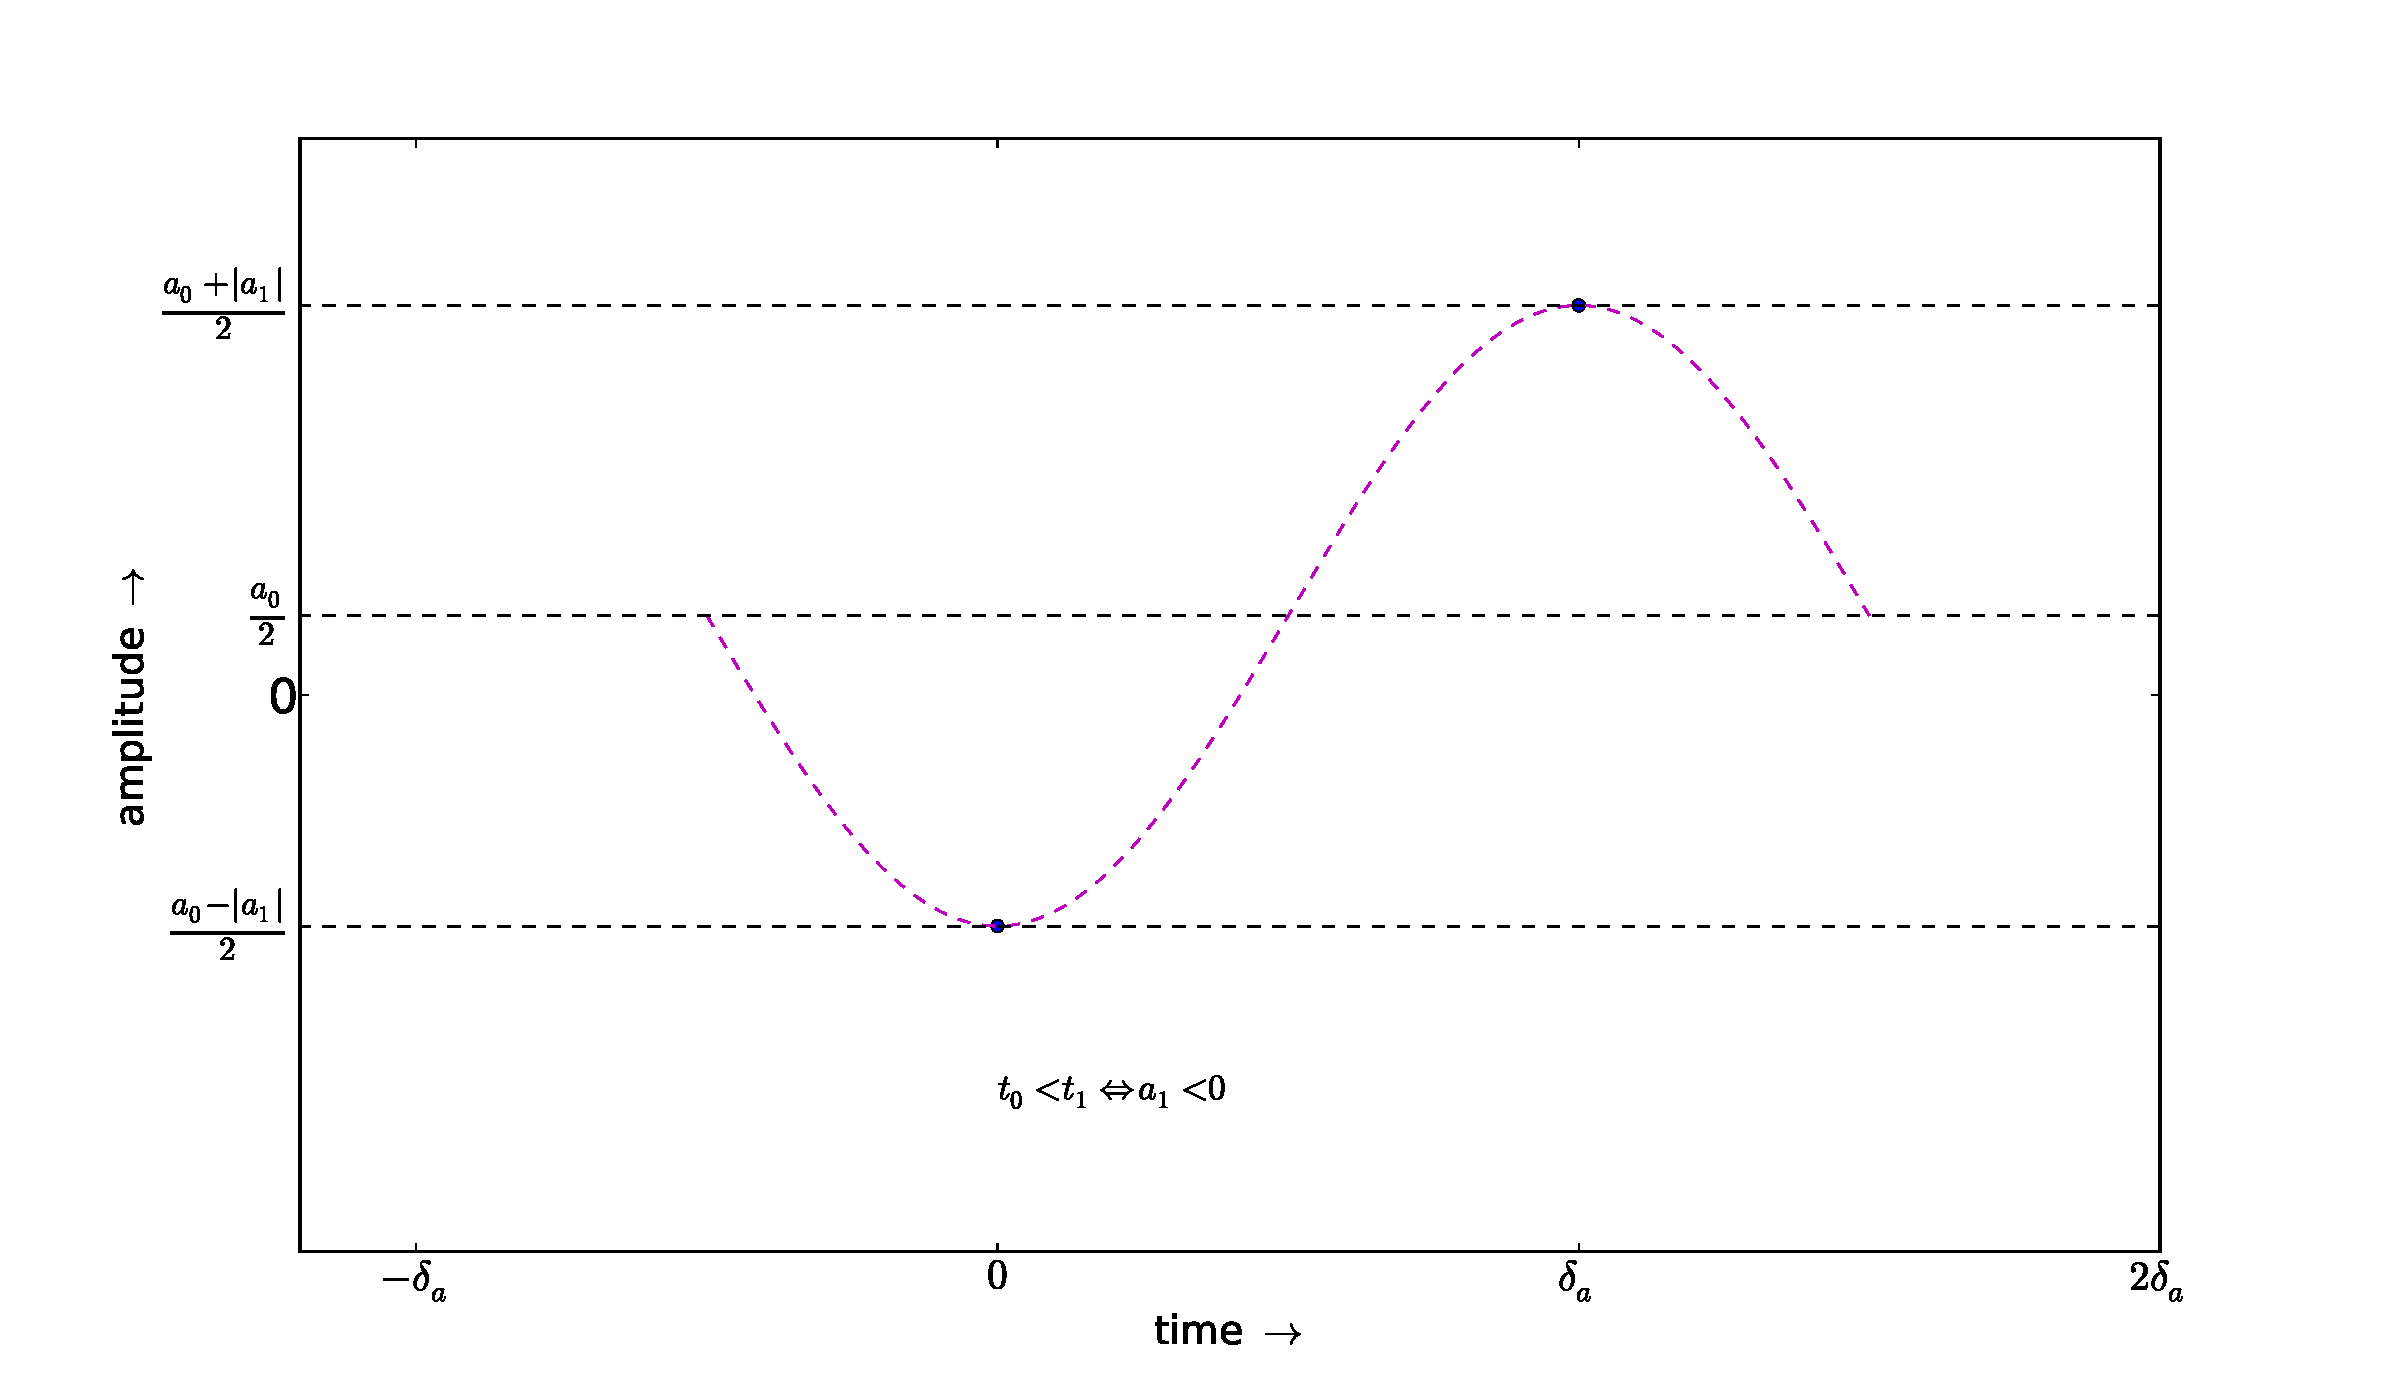
\includegraphics[width=\columnwidth]{figures/amostras2c__}
     \caption{Oscillation of 2 samples (maximum frequency for any $f_a$). The first coefficient reflects a detachment (\emph{offset} or \emph{bias}) and the second coefficient specifies the oscillation amplitude.}
         \label{fig:amostras2}
 \end{figure}

Figure~\ref{fig:amostras2} shows two samples and its spectral components. In this case, the Fourier decomposition has one unique pair of coefficients $\{c_k=a_k-j.b_k\}_0^{\Lambda-1=1}$ relative to frequencies $\{f_k\}_0^1=\left\{w_k\frac{f_a}{2\pi}\right\}_0^1=\left\{k\frac{f_a}{\Lambda=2}\right\}_0^1=\left\{0,\frac{f_a}{2}=f_{\text{max}}\right\}$
with energies $e_k=\frac{(c_k)^2}{\Lambda=2}$. The role of amplitudes $a_k$ is clearly observed with $\frac{a_0}{2}$, the fixed offset\footnote{Also called \emph{bias}.} and $\frac{a_1}{2}$, oscillation amplitude with frequency given by the relation $f_k=k \frac{f_a}{\Lambda=2}$.
This case have special relevance. It is necessary at least 2 samples to represent an oscillation and it yields the Nyquist frequency $f_{\text{max}}=\frac{f_a}{2}$, which is the maximum frequency in a sound sampled with $f_a$ samples per second\footnote{Any sampled signal has this property, not only the digitalized sound.}.

All fixed sequences $T_i$ of only $3$ samples also have just $1$ frequency, since their first harmonic has $1,5$ samples and exceeds the bottom limit of 2 samples, i.e.\ the frequency of the harmonic would exceed the Nyquist frequency:  $\; \frac{2. f_a}{3} > \frac{f_a}{2} $. 
The coefficients $\{c_k\}_0^{\Lambda-1=2}$ are present in 3 frequency components. One is relative to zero frequency ($c_0$), and the other two ($c_1$ and $c_2$) have the same role for the reconstruction of sinusoid with $f=f_a/3$.

 \begin{figure}[h!]
     \centering
         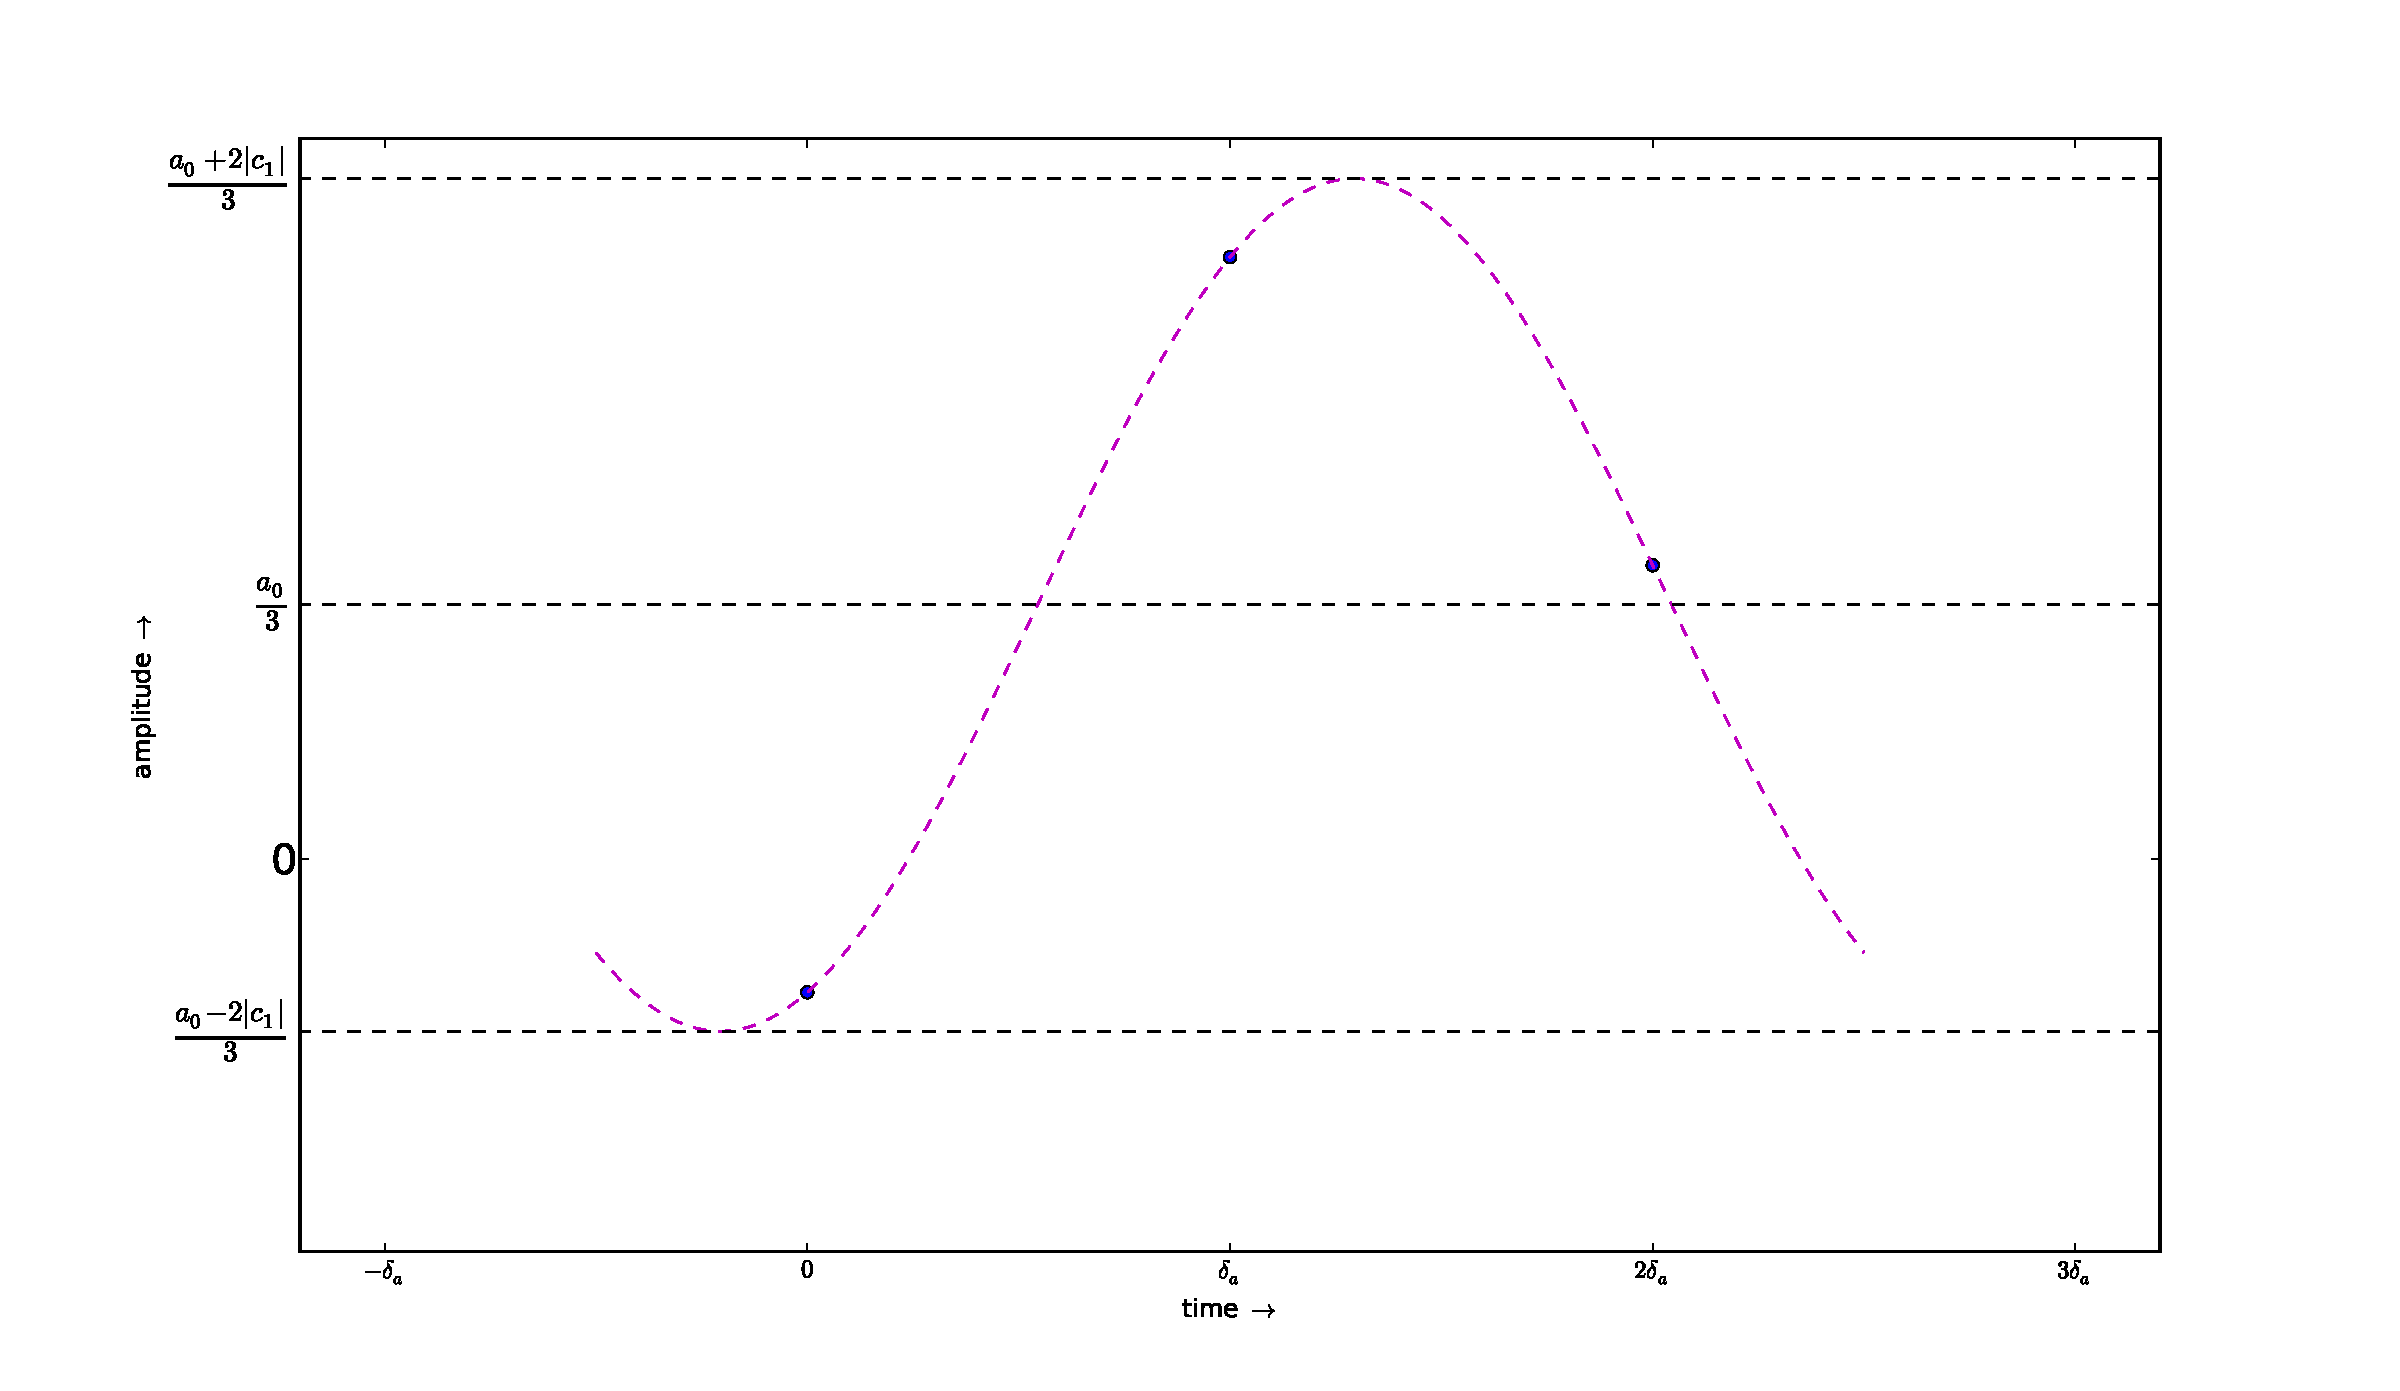
\includegraphics[width=\columnwidth]{figures/amostras3b}
     \caption{Three fixed samples presents only one non-null frequency. $c_1=c_2^*$ and $w_1 \equiv w_2$.}
         \label{fig:amostras3}
 \end{figure}

$\Lambda$ real samples $t_i$ result in $\Lambda$ complex coefficients $c_k=a_k+j.b_k$. The coefficients $c_k$ are equivalent two by two, corresponding to the same frequencies and with same contribution to its reconstruction. They are complex conjugates: $a_{k1}=a_{k2}$ and $b_{k1}=-b_{k2}$ and, as a consequence, the modules are equal and phases have opposite signs. Remembering that $f_k = k\frac{f_a}{\Lambda}, \; k \in \left\{0, ..., \left \lfloor \frac{\Lambda}{2} \right \rfloor \right\} $. When $k > \frac{\Lambda}{2}$, the frequency $f_k$ is mirrored by $\frac{f_a}{2}$ in this way: $f_k=\frac{f_a}{2} - (f_k-\frac{f_a}{2})=f_a-f_k=f_a - k\frac{f_a}{\Lambda}=(\Lambda-k)\frac{f_a}{\Lambda} \;\;\;\; \Rightarrow \;\;\;\; f_k\equiv f_{\Lambda-k} \; ,\;\; \forall \;\; k<\Lambda$. 

The same can be observed with $w_k=f_k.\frac{2\pi}{f_a}$ and the periodicity $2\pi$: it follows that $w_k=-w_{\Lambda-k} \; ,\;\; \forall \;\; k<\Lambda$. Given the cosine (an even function) and the inverse tangent (an odd function), the components in $w_k$ and $w_{\Lambda-k}$ contribute with coefficients $c_k$ and $c_{\Lambda-k}$ in the reconstruction of the real samples.

In other words, in a decomposition of $\Lambda$ samples, the $\Lambda$ frequency components $\{c_i\}_0^{\Lambda-1}$ are equivalents in pairs,
except for $f_0$, and, when $\Lambda$ is even, for $f_{\Lambda/2}=f_{\text{max}}=\frac{f_a}{2}$. Both components are isolated, i.e.\ there is one and only component in frequency $f_0$ or $f_{\Lambda/2}$ (if even $\Lambda$). 
One can verify this assertion considering $k=0$ and $k=\Lambda/2$. Uncoiled: $f_{\Lambda/2}=f_{(\Lambda-\Lambda/2) = \Lambda/2}$ and $f_0=f_{(\Lambda-0)=\Lambda}=f_0$.
Furthermore, these two frequencies (zero and Nyquist frequency) does not have phase variation, being their coefficients strictly real. In this way, it is possible to conclude the number $\tau$ of equivalent coefficient pairs:

\begin{equation}\label{coefsPareados}
\tau = \frac{\Lambda - \Lambda \% 2}{2} +\Lambda \% 2 -1
\end{equation}

This discussion makes clear the equivalences ~\ref{equivalenciasFreqs}, ~\ref{equivalenciasModulos} and ~\ref{equivalenciasFases}:

\begin{equation}\label{equivalenciasFreqs}
f_{k}\equiv f_{\Lambda-k}\;, \;\; w_{k}\equiv-w_{\Lambda-k}\;\;\;, \quad \;\; \forall \quad 1 \leq k \leq \tau  
\end{equation}

\begin{figure*}
    \centering
        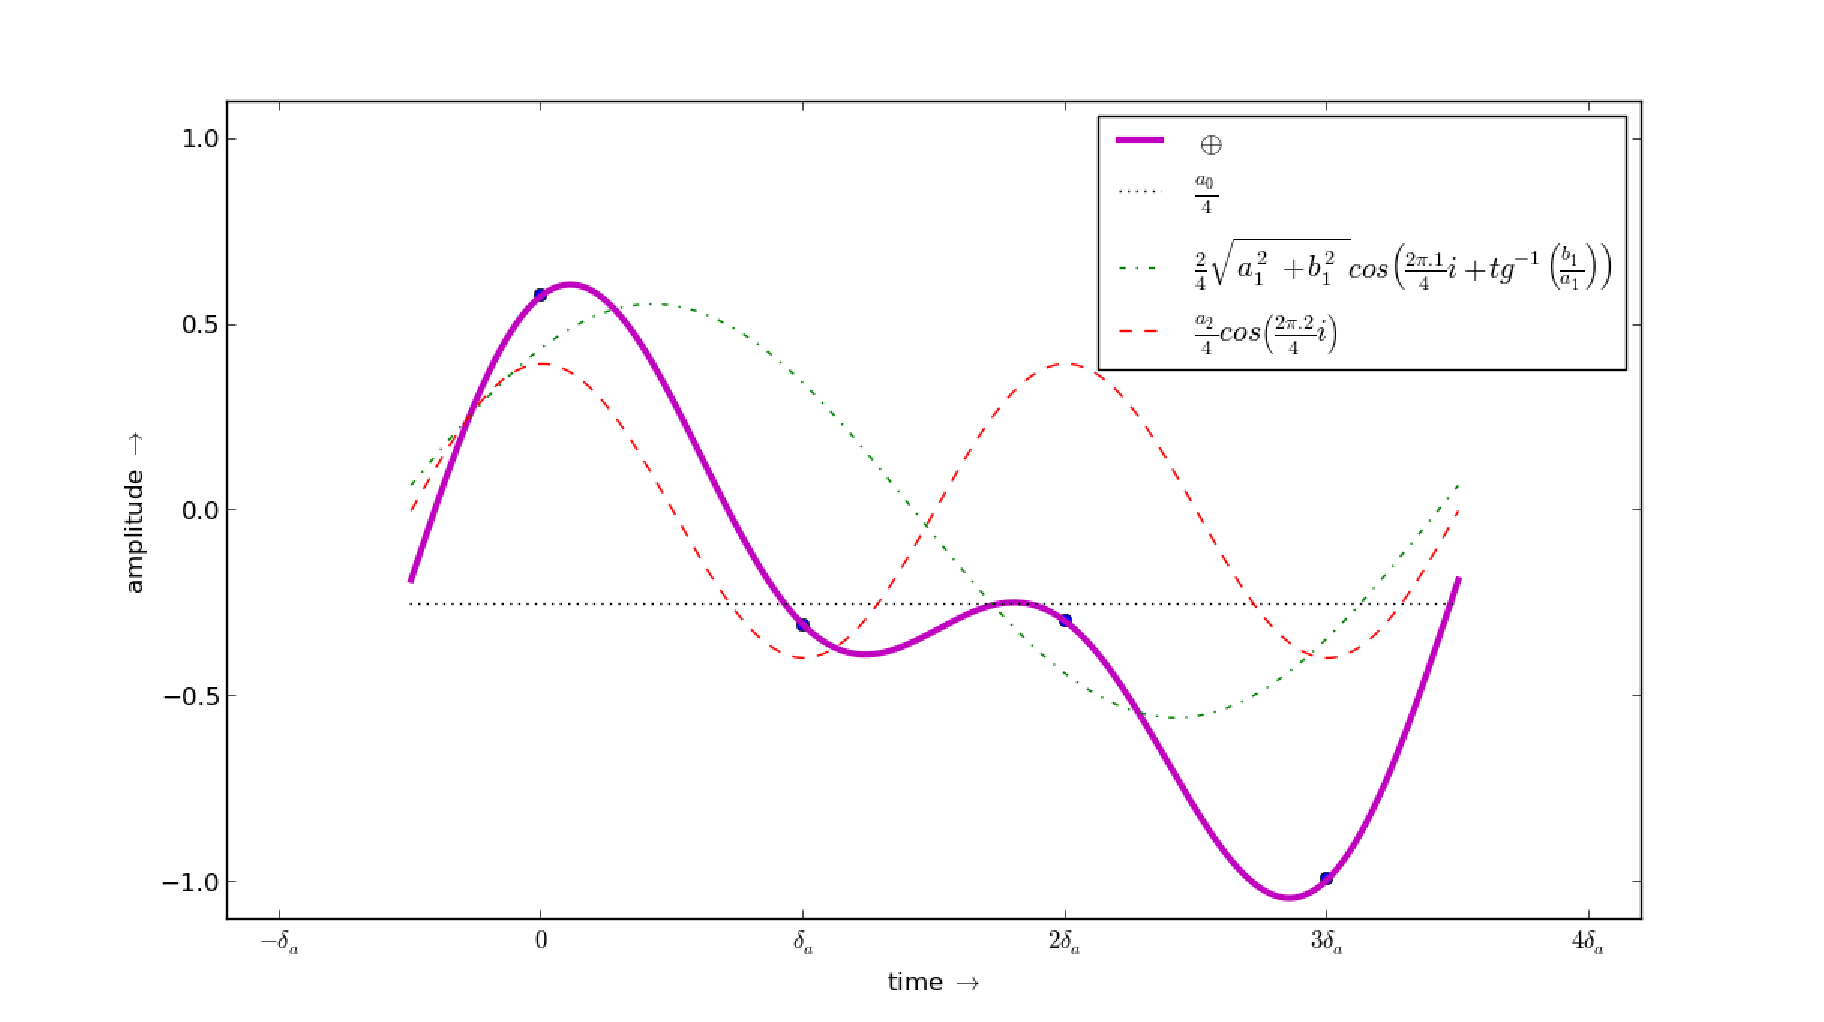
\includegraphics[width=\textwidth]{figures/amostras4___}
    \caption{Frequency components for 4 samples.}
        \label{fig:amostras4}
\end{figure*}

$T_i \; \Rightarrow \; a_k = a_{\Lambda -k}\;\;$ and $\;\;b_k = - b_{\Lambda -k}$, and thus:

\begin{equation}\label{equivalenciasModulos}
\sqrt{a_k^2 + b_k^2} = \sqrt{a_{\Lambda - k}^2 + b_{\Lambda -k}^2} \;\;, \quad \;\; \forall \quad 1 \leq k \leq \tau  \\
\end{equation}

\begin{equation}\label{equivalenciasFases}
tg^{-1}\left(\frac{b_k}{a_k}\right)=-tg^{-1}\left(\frac{b_{\Lambda -k}}{a_{\Lambda - k}}\right)\;\;,\quad \;\; \forall \quad 1 \leq k \leq \tau
\end{equation}

with $k \in \mathbb{N}$.

To expose the general case for components combination in each sample $t_i$, one can gather relations in equation~\ref{moduloEfase} for the real signal reconstruction, relations of modules~\ref{equivalenciasModulos} and phases equivalences~\ref{equivalenciasFases}, the number of paired coefficients~\ref{coefsPareados}, and equivalence of paired frequencies~\ref{equivalenciasFreqs}:

\begin{multline}\label{eq:reconsCompleta}
t_i = \frac{a_0}{\Lambda} + \frac{2}{\Lambda}\sum_{k=1}^{\tau}\sqrt{a_k^2 + b_k^2} \; cos\left[w_k i - tg^{-1}\left(\frac{b_k}{a_k}\right)\right]+ \\ \frac{ a_{\Lambda/2}}{\Lambda}.(1-\Lambda\% 2)
\end{multline}

with $a_{\Lambda/2}=0$ if $\Lambda$ odd.

\begin{figure*}
    \centering
        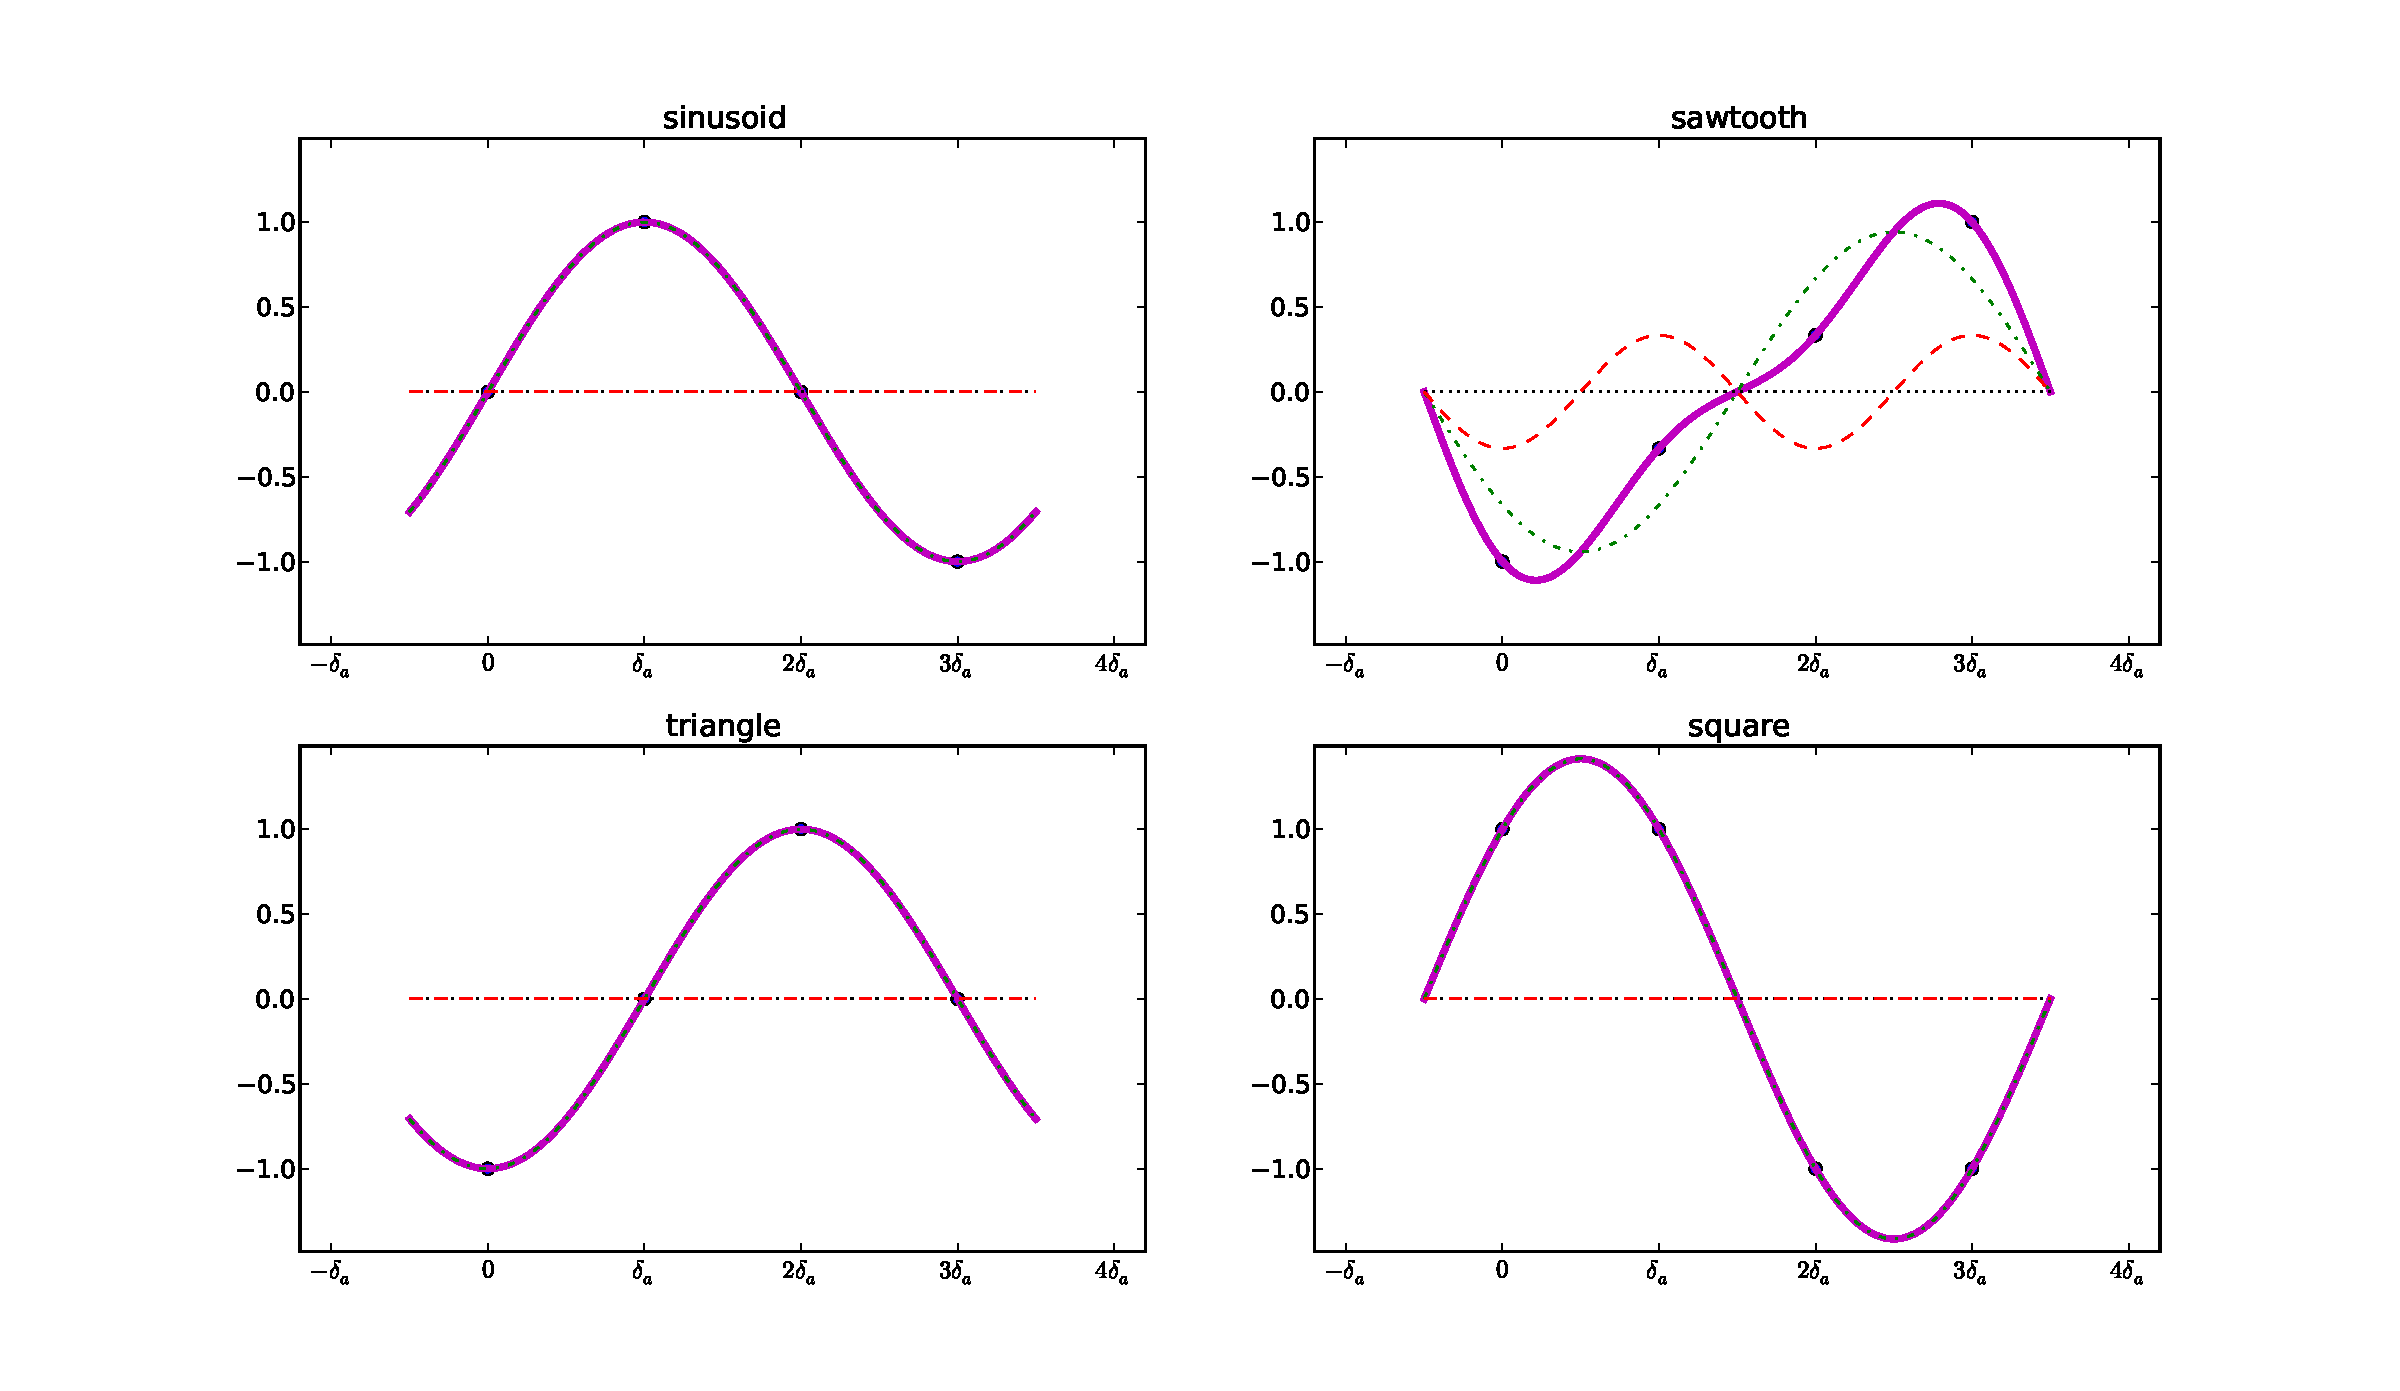
\includegraphics[width=\textwidth]{figures/amostras4formas__}
    \caption{Basic wave forms with 4 samples.}
        \label{fig:formas4}
\end{figure*}

With 4 samples it is possible to represent 1 or 2 frequencies in any proportions (i.e. with independence). Figure~\ref{fig:amostras4} depicts the basic waveforms with 4 samples and its two (possible) components. The individual contributions sum to the original waveform and a brief inspection reveals the major curvatures resulting from the higher frequency, while the fixed offset is captured in the zero frequency component.

\begin{figure*}
    \centering
        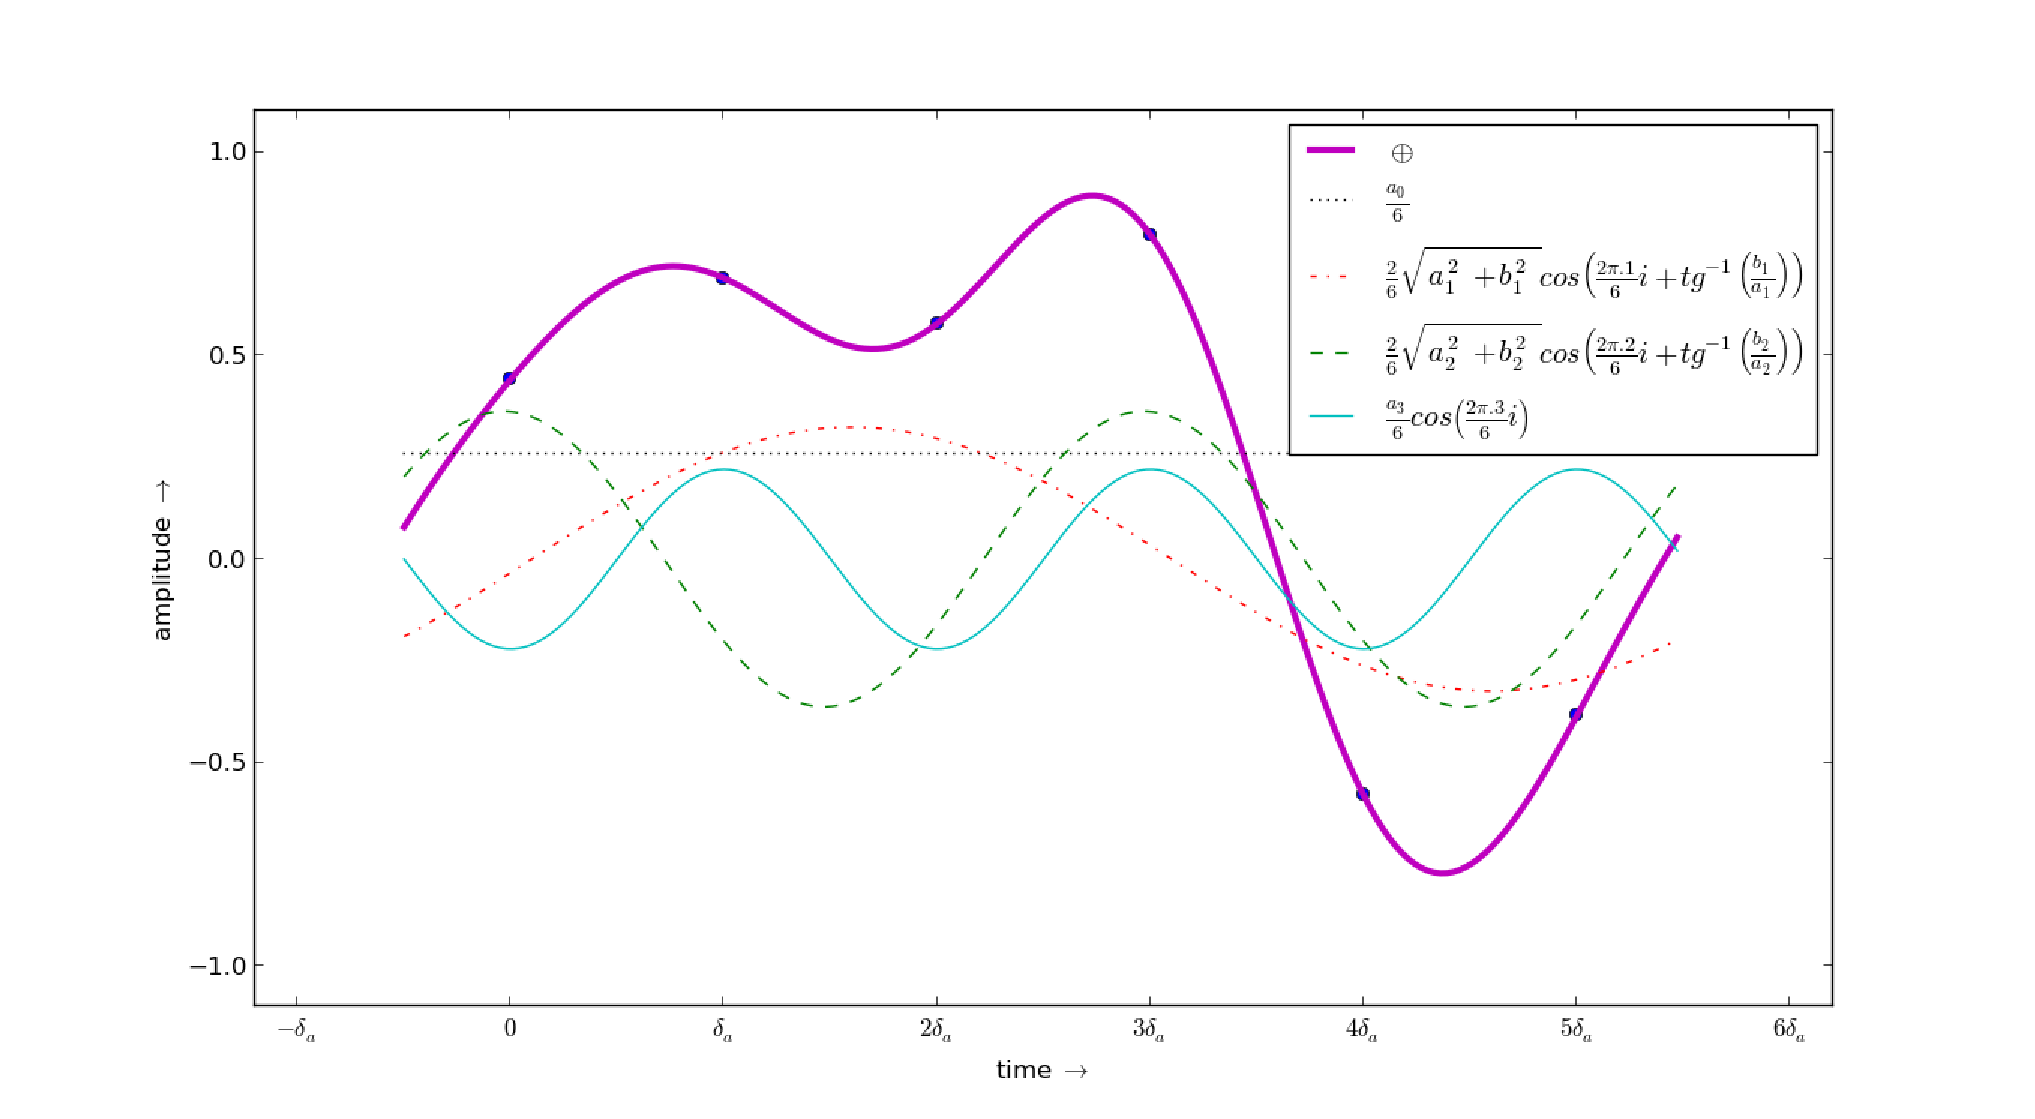
\includegraphics[width=\textwidth]{figures/amostras6_}
    \caption{Frequency components for 6 samples: 4 sinusoids, one of them is the \emph{bias} with zero frequency.}
        \label{fig:amostras6}
\end{figure*}

Figure~\ref{fig:formas4} shows the harmonics for the basic waveforms of equations~\ref{senoide},~\ref{denteDeSerra},~\ref{triangular} and~\ref{quadrada} for the case of 4 samples. There is only 1 sinusoid for each waveform, with the exception of the sawtooth, which has even harmonics.

Figure~\ref{fig:amostras6} presents the sinusoidal decomposition for 6 samples and figure~\ref{fig:formas6} presents the decomposition of the basic wave forms.
In this case, the waveforms have spectra with fundamental differences: square and triangular have the same components but with different proportions, while the sawtooth have an extra component.

\begin{figure}[h!]
    \centering
        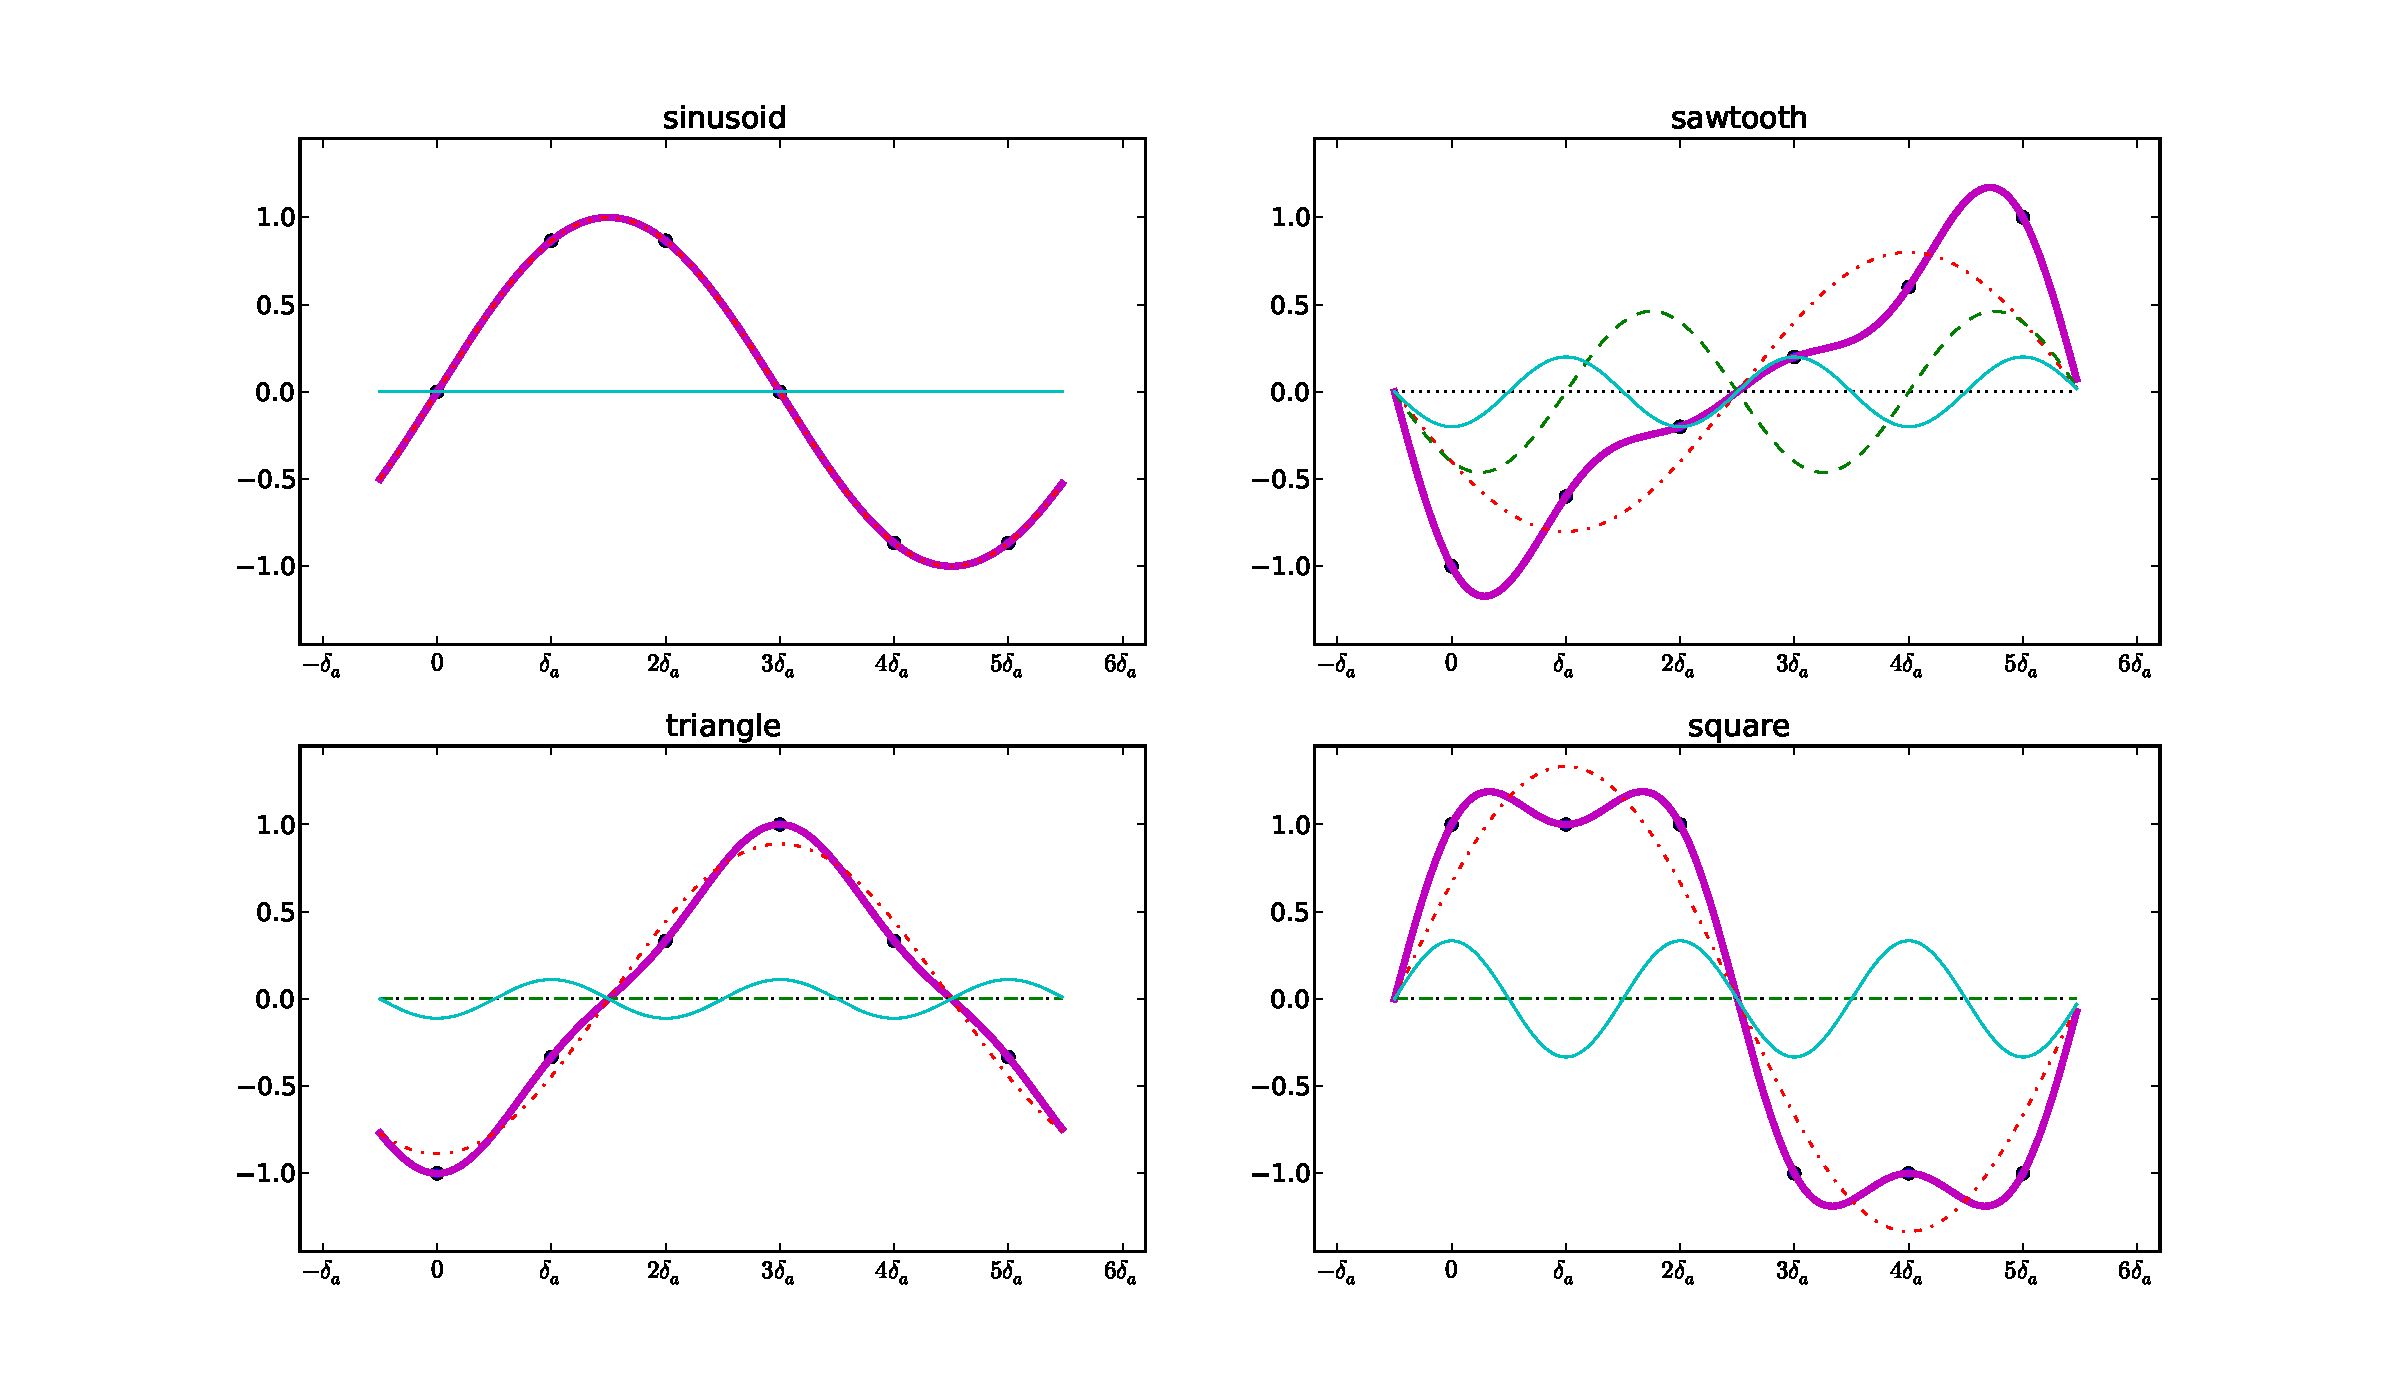
\includegraphics[width=\columnwidth]{figures/amostras6formas__}
    \caption{Basic waveforms with 6 samples: triangular and square waveforms have odd harmonics, with different proportions and phases; the sawtooth has even harmonics.}
        \label{fig:formas6}
\end{figure}

%%%%%%%%%%%%%%%%%%%%%%%%%%%%%%%
\subsection{The basic note}\label{notaBasica}

Be $f$ such that it divides $f_a$\footnote{As pointed before, this limitation simplify the explanation without losing generality, and will be overcome in the next section.}. A sequence $T_i$ of sonic samples separated by $\delta_a=1/f_a$ describes a musical note with a frequency of $f$ Hertz and $\Delta$ seconds of duration if, and only if, it has the periodicity $\lambda_f=f_a/f$ and size $\Lambda=\lfloor f_a . \Delta \rfloor $:

\begin{equation}\label{eq:notaBasica}
T_i^{f,\; \Delta}=\{t_{i \, \% \lambda_f} \}_0^{\Lambda-1}= \left \{t^f_{i \; \% \left( \frac{f_a}{f} \right) } \right \}_0^{\Lambda-1}
\end{equation}

The note by itself does not specify a timbre. Nevertheless, it is necessary to choose a waveform for the samples $t_i$ to have a value. An unique period from the basic waveforms can be used to specify the note, where $\lambda_f=\frac{f_a}{f}$ is the number of samples at the period. Here, $L_i^{f,\, \delta_f} $ is the sequence that describes a period of the waveform $L_i^f \in \{S_i^f,Q_i^f,T_i^f,D_i^f,R_i^f \}$ with duration $\delta_f=1/f$ (as given by equations~\ref{senoide}, ~\ref{denteDeSerra}, ~\ref{triangular} and ~\ref{quadrada}) and $R_i^f$ is a sampled real waveform:

\begin{equation}\label{periodoUnico}
L_i^{f , \delta_f } = \left\{ l_i^f \right\}_0^{\delta_f . f_a -1}=\left\{ l_i^f \right\}_0^{\lambda_f-1}
\end{equation}

Therefore, the sequence $T_i$ will consist in a note of duration $\Delta$ and frequency $f$ if:

\begin{equation}\label{eq:notaBasicaTimbre}
T_i^{f,\; \Delta}=\left\{t_i^f\right\}_0^{\lfloor f_a . \Delta \rfloor -1}=\left \{ l^f_{i\,\%\left(\frac{f_a}{f}\right)} \right \}_0^{\Lambda-1}
\end{equation}

\subsection{Spatial localization and spatialization}\label{subsec:spac}

Although it is not one of its four basic properties, a musical note always has a spatial localization: the note source position at the ordinary physical space. The existence of an environment that reverberates the note is the matter of 'spatialization'. Both fields, spatialization and spatial localization, are widely valued by audiophiles and music industry~\cite{floEsp}. 

\subsubsection{Spatial localization}

It is understood that the perception of sound localization occurs in our nervous system by three informations: the delay of incoming sound between both ears, the difference of sound intensity at each ear and the filtering realized by the human body, including its chest, head and ears~\cite{Roederer, hrtf, Heeger}. 

\begin{figure}[h!]
    \centering
        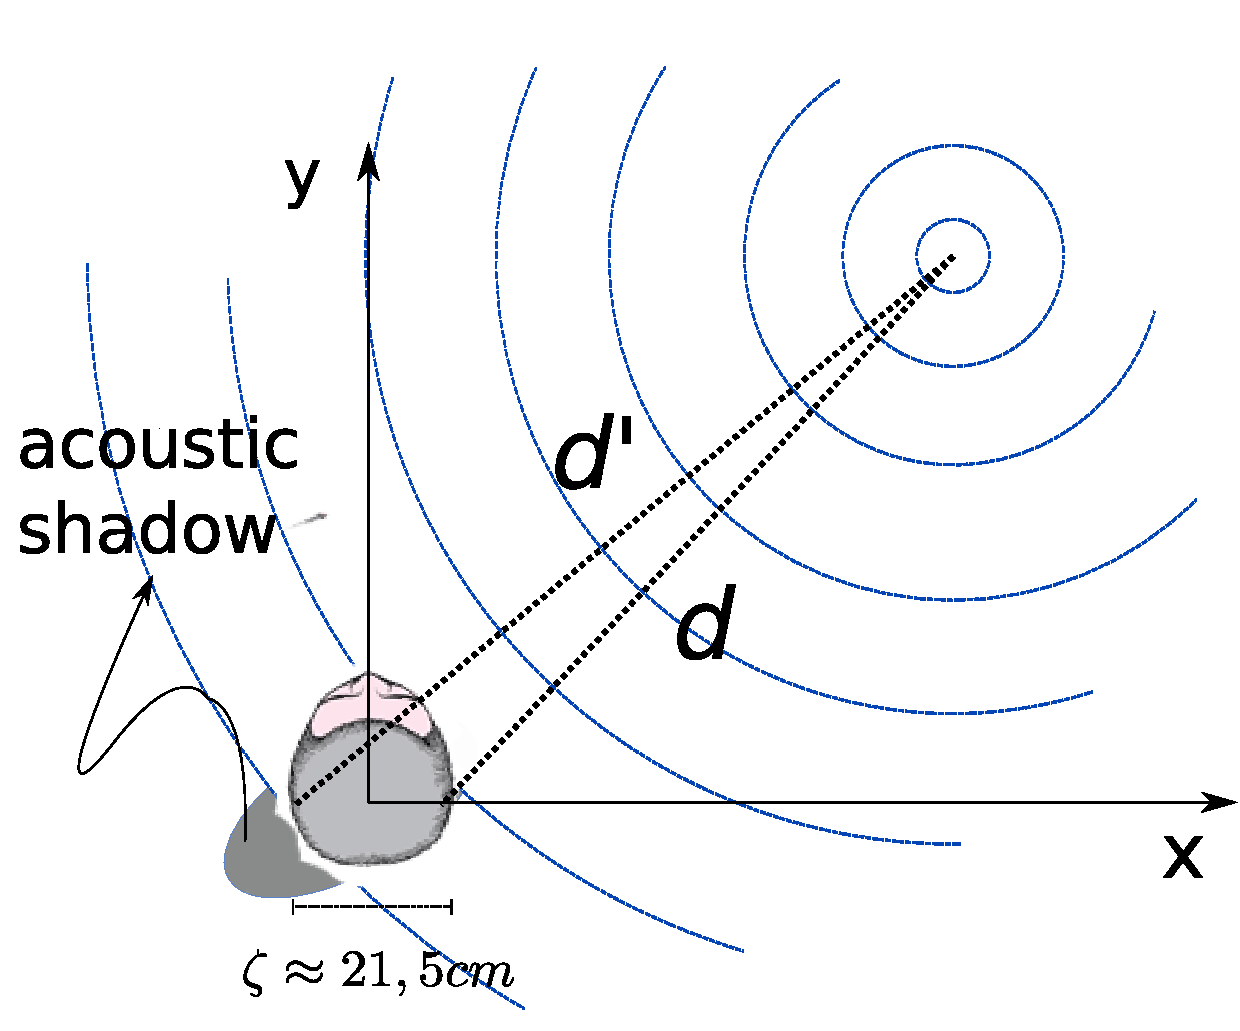
\includegraphics[width=.5\textwidth]{figures/espacializacao___}
    \caption{Detection of sound source localization: schema used to calculate Interaural Time Difference (ITD) and Interaural Intensity Difference (IID).}
    \label{fig:spac}
\end{figure}

Considering only the direct incidences in each ear, the equations are quite simple. An object placed at $(x,y)$, as in figure~\ref{fig:spac}, is distant of each ear by:

\begin{equation}\label{eq:distOuvidos}
\begin{split}
d & =\sqrt{\left (x-\frac{\zeta}{2} \right )^2+y^2} \\
d' & =\sqrt{\left (x+\frac{\zeta}{2} \right )^2 + y^2}
\end{split}
\end{equation}

Where $\zeta$ is the distance between ears $\zeta$,  known to be $\zeta \approx 21,5cm$ in an adult human.
Immediate calculations result in the ITD:

\begin{equation}\label{eq:dti}
ITD=\frac{d'-d}{v_{sound\;at\;air}\approx 343.2 }\quad \text{seconds}
\end{equation}

\noindent and in the Interaural Intensity Difference:

\begin{equation}\label{eq:dii}
IID=20\log_{10}\left (\frac{d}{d'}\right) \quad decibels
\end{equation}

\noindent which, converted to amplitude, yields $IID_a=\frac{d}{d'}$. The $IID_a$ can be used as a multiplicative constant to the right channel of a stereo sound signal: $\{t_i'\}_0^{\Lambda -1}=\{IID_a . t_i\}_0^{\Lambda -1}$, where $\{t_i'\}$ are samples of the wave incident in the left ear. It is possible to use IID together with ITD as a time advance for the right channel. It is a crucial vestige to localization perception of bass sounds and percussive sonorities~\cite{Heeger}. 
With $\Lambda_{ITD}=\lfloor ITD . f_a \rfloor$:

\begin{equation}\label{eq:locImpl}
\begin{split}
\Lambda_{ITD} & = \left \lfloor \frac{d'-d}{343,2}  f_a \right \rfloor \\
IID_a & = \frac{d}{d'} \\
\left\{t_{(i+\Lambda_{ITD})}'\right\}_{\Lambda_{ITD}}^{\Lambda+\Lambda_{ITD}-1} & =\left\{IID_a . t_i\right\}_0^{\Lambda-1} \\
\left\{t_i'\right\}_0^{\Lambda_{ITD}-1} & = 0
\end{split}
\end{equation}

\noindent with $t_i$ as the right channel and $t_i'$ the left channel. If $\Lambda_{ITD} < 0 $, it is only needed to change $t_i$ by $t_i'$ and to use $\Lambda_{ITD}'= | \Lambda_{ITD} | $ and $IID_a'=1 / IID_a$.

Although simple until here, spatial localization depends considerably of other cues. By using only ITD and IID it is possible to specify solely the horizontal angle (azimuthal) $\theta$ given by:

\begin{equation}\label{eq:angulo}
\theta=\tan^{-1}\left ( \frac{y}{ x }  \right )
\end{equation}

\noindent with $x,y$ as presented in Figure~\ref{fig:spac}. Henceforth, there are problems when $\theta$ fall upon the so called "cone of confusion": the same pair of ITD and IID results in a large number of points inside the cone. On those points the inference of the azimuthal angle depends specially of the attenuative filtering for high frequencies, since the head interferes much more in the treble than in bass waves~\cite{Heeger,hrtf}. Also relevant to the hearing of lateral sources is that low frequencies diffracts and the wave arrive to the opposite ear with a delay of $\approx 0,7ms$.\cite{floEsp}

Figure~\ref{fig:spac} depicts the acoustic shadow of the cranium, an important phenomenon to perception of source azimuthal angle in the cone of confusion. The cone itself is not shown in figure~\ref{fig:spac} because it is not exactly a cone and its precise dimensions were not encountered in the literature. Given the filtering and diffraction dependent of the sound spectrum, it is hard, if not impossible, to correctly draw the confusion cone. Even so, the cone of confusion can be understood as a cone with its top placed in the middle of head and growing out in the direction of each ear~\cite{hrtf}.

On the other hand, the complete localization, including height and distance of sound source, is given by the Head Related Transfer Function (HRTF)~\cite{hrtf}. There are well known open databases of HRTF, such as CIPIC, and it is possible to apply those transfer functions in a sonic signal by convolution (see equation~\ref{eq:conv})~\cite{CIPIC}. Each human body has its filtering and there are techniques to generate HRTFs to be universally used~\cite{lazaSPA}. 

\subsubsection{Spatialization}

Spatialization results from sound reflections and absorptions by room/environment surface where the note is played. The sound propagates through the air with a speed of $\approx 343,2m/s$ and can be emitted from a source with any directionality pattern. When a sound pulse encounters a surface there is reflection. In this reflection occurs: 1) the inversion of propagation speed component that is normal to the surface;  2) energy absorption, specially in trebles. The sonic waves propagate until they reaches inaudible levels (and even further). As a sonic front reaches the human ear, it  can be described as the original sound, with the last reflection point as the source, and the absorption filters of each surface it has reached. It is possible to simulate reverberations that are impossible in real systems. For example, it is possible to use asymmetric reflections with relation to the axis perpendicular to the surface, or to increase specific frequency bands (known as 'resonances'), both characteristics are not found in real systems.

There are some reverberation models that are less related to each independent reflection, exploring valuable information to the auditory system. In fact, reverberation can be modeled with a set of 2 temporal and spectral sections:

\begin{itemize}
   \item First period: 'first reflections' are more intense and scattered.
   \item Second period: 'late reverberation' is practically a dense succession of indistinct delays with exponential decay and statistical occurrences.
   \item First band: the bass has some resonance bandwidths relatively spaced.
   \item Second band: mid and treble have progressive decay and smooth statistical fluctuations.
\end{itemize}

Smith III points that reasonable concert rooms have total reverberation time of  $\approx 1.9$ seconds, and that the period of first reflections is around $0.1$ seconds. These values suggest that, in the given conditions, there are perceived wave pulses which propagates for $652.08$ meters long ($83.79k$ samples in $f_a=44.1kHz$) before reaching the ear. In addition, sound reflections made after propagation for $34.32$ meters long ($4.41k$ samples in $f_a=44.1kHz$) have incidences less distinct by hearing. These first reflections are particularly important to spacial sensation. The first incidence is the direct sound, described by ITD and IID of equations~\ref{eq:dti} and~\ref{eq:dii}. Admitting that each one of the first reflections, before reaching the ear, will propagate at least $3-30m$, dependent of room dimension, the separation between the first reflections is $8-90ms$ ($\approx 350-4000$ samples in $f_a=44.1kHz$). It is possible to experimentally verify that the number of reflections increases with squared proportion $\approx k.n^2$. A discussion about the use of convolutions and filtering to favor implementation of these phenomena is provided in subsection~\ref{subsec:mus2}, specially at the paragraphs about reverberation.

\subsection{Musical use}\label{subsec:basMus}

Once defined the basic note, it is convenient to build musical structures with sequences based on these particles. The sum of elements with same index of $N$ sequences $T_{k,i}=\{t_{k,i}\}_{k=0}^{N-1}$ with same size $\Lambda$ results in the overlapped spectral contents of each sequence, in a process called mixing:

\begin{equation}\label{eq:mixagem}
\{t_i\}_0^{\Lambda-1}=\left \{ \sum_{k=0}^{N-1}t_{k,i} \right \}_0^{\Lambda-1}
\end{equation}

\begin{figure}[h!]
    {\centering
        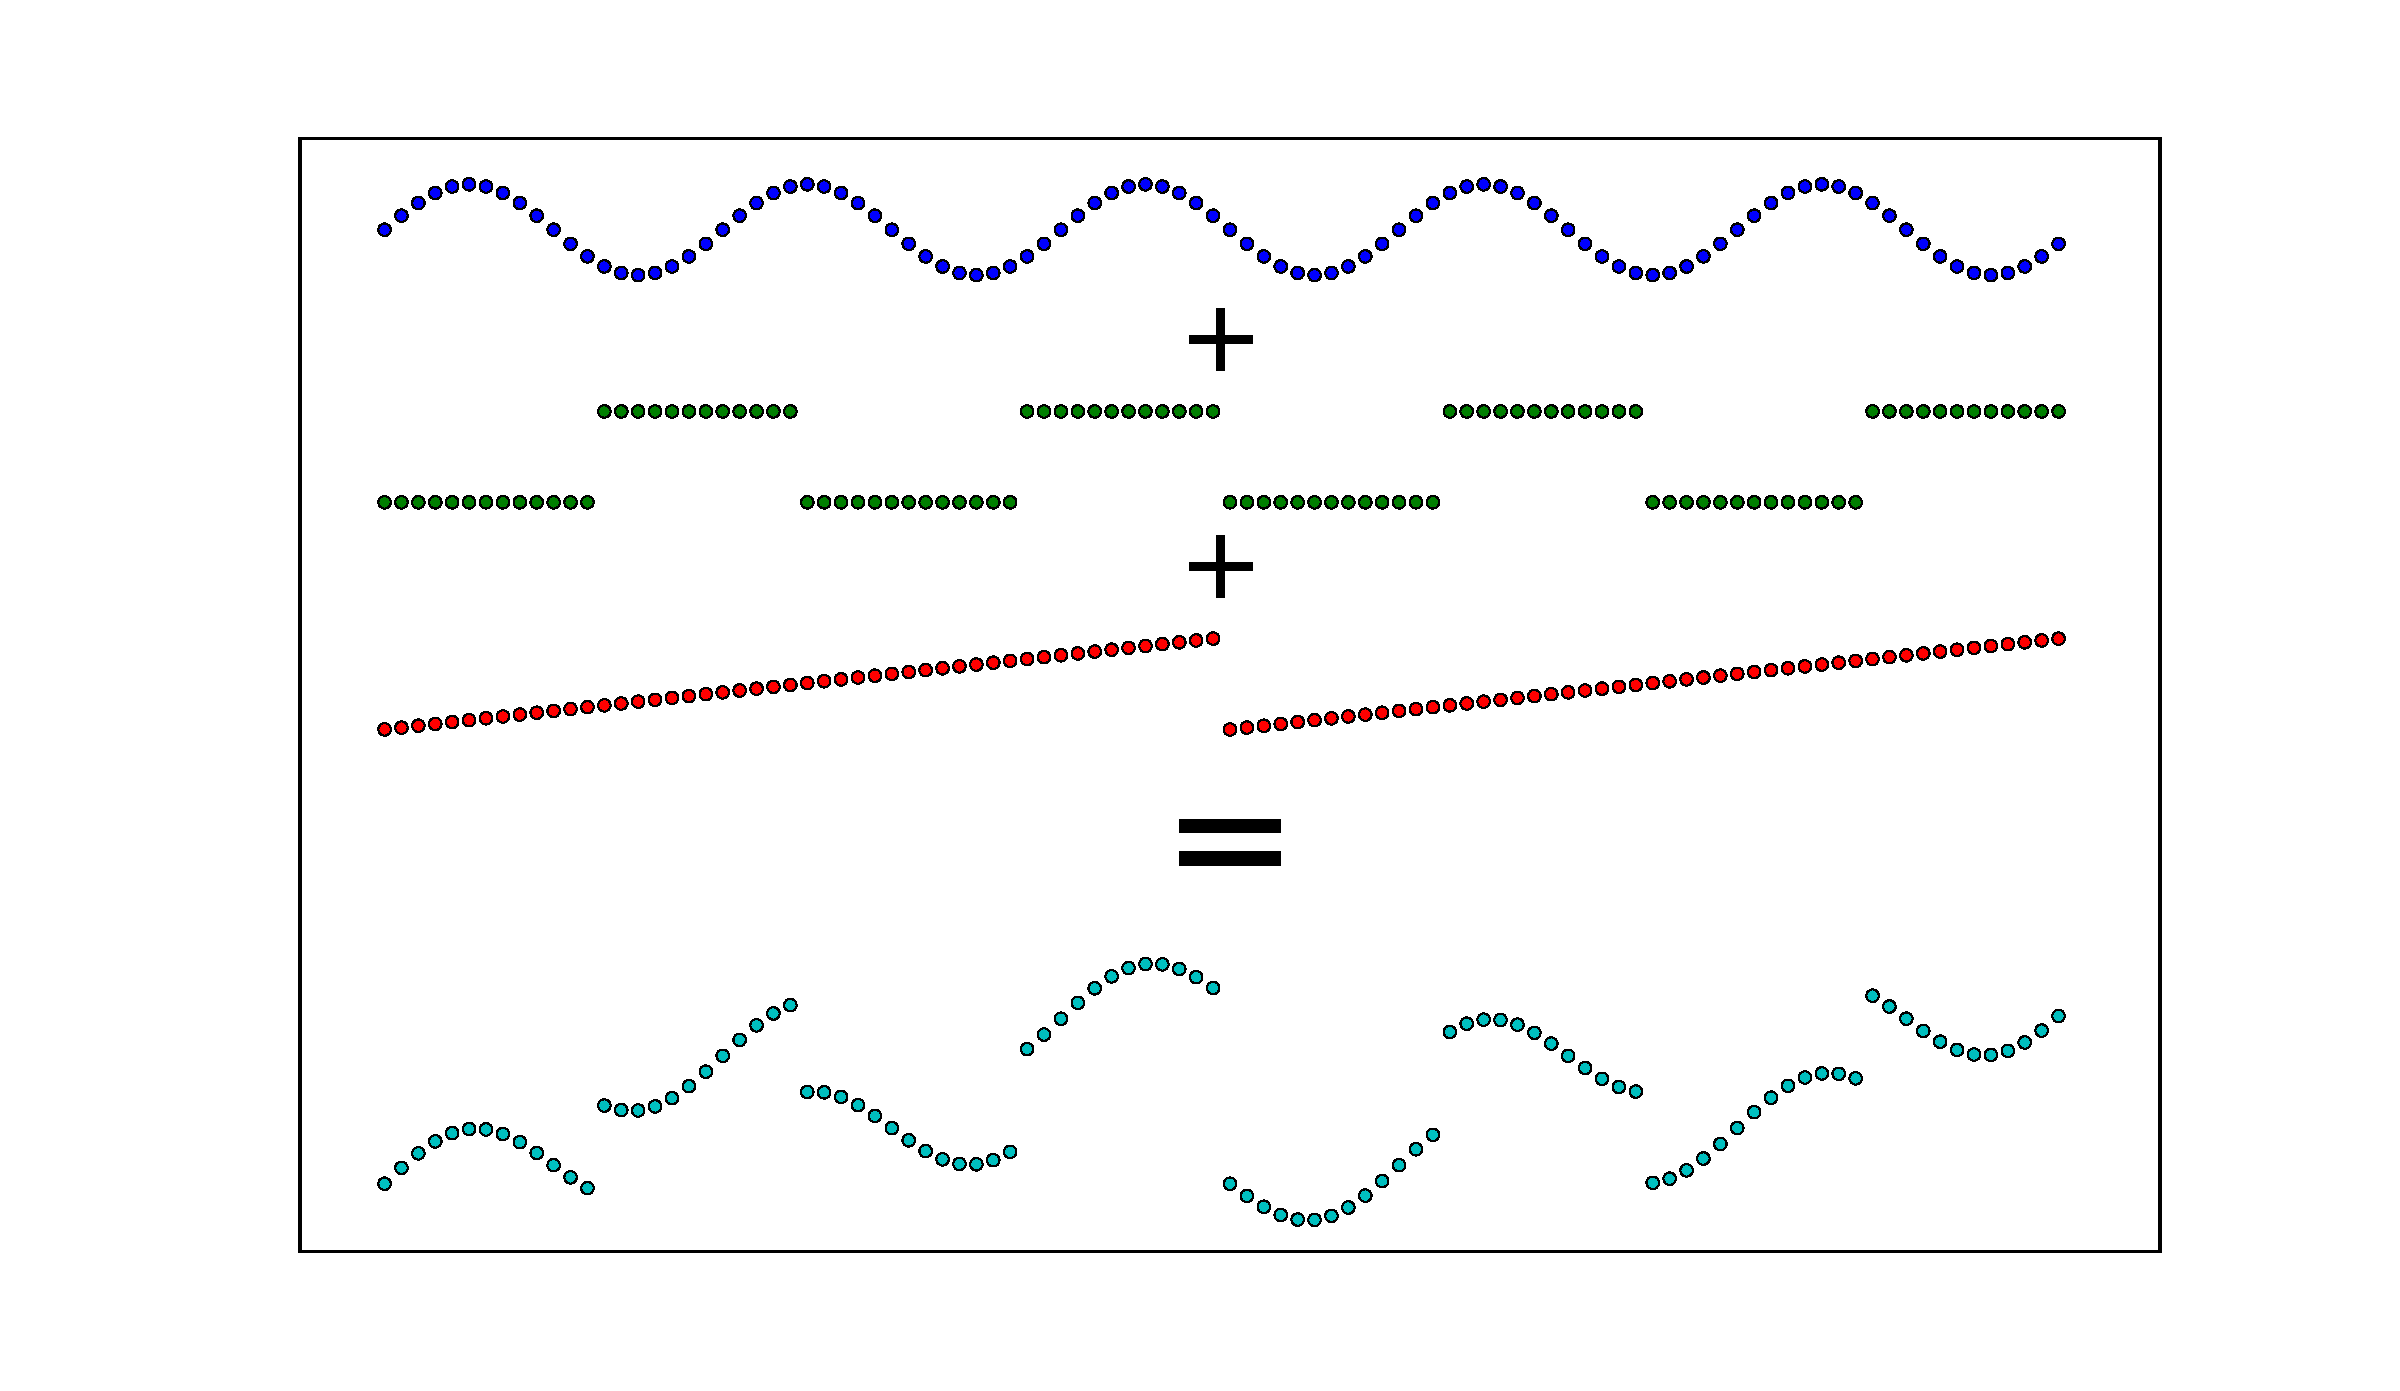
\includegraphics[width=\columnwidth]{figures/mixagem}}
    \caption{Mixing of three sound sequences. The amplitudes are directly overlapped.}
        \label{fig:mixagem}
\end{figure}

Figure~\ref{fig:mixagem} illustrates this overlapping process of discretized sound waves, each with 100 samples. It is possible to conclude that, if $f_a=44.1kHz$, the frequencies of the sawtooth, square and sine wave are, respectively: $\frac{f_a}{100/2}=882Hz$, $\frac{f_a}{100/4}=1764Hz$ and $\frac{f_a}{100/5}=2205Hz$. The samples duration are very short $\frac{f_a=44.1kHz}{100} \approx 2 \text{ milliseconds}$. One can complete the sequence with zeros to sum (mix) sequences with different sizes.

The mixed notes are generally separated by the ear according to the physical laws of resonance and by the nervous system~\cite{Roederer}.  This musical notes mixing process results in musical harmony whose intervals between frequencies and chords of simultaneous notes guide subjective and abstract aspects of music and its appreciation~\cite{Harmonia}, which is tackled in section~\ref{sec:notesMusic}. 

Sequences can be concatenated in time. If the sequences $\{t_{k,i}\}_0^{\Lambda_k-1}$ of size $\Lambda_k$ represent $k$ musical notes, their concatenation in a unique sequence $T_i$ is a simple melodic sequence, or melody of its own:

\begin{equation}\label{eq:concatenacao}
\begin{split}
\{t_i\}_0^{\sum\Delta_k-1}= & \{t_{l,i}\}_0^{\sum\Delta_k-1}, \;\; \\ l\text{ smallest integer } : & \quad \Lambda_l > i -\sum_{j=0}^{l-1}\Lambda_j
\end{split}
\end{equation}

This mechanism is demonstrated in Figure~\ref{fig:concatenacao} with same sequences of Figure~\ref{fig:mixagem}. Although the sequences are short for the usual sample rates, it is easy to observe the concatenation of sound sequences. Besides that, each note has a duration larger than $100ms$ if $f_a<1kHz$.

\begin{figure}[h!]
{    \centering
        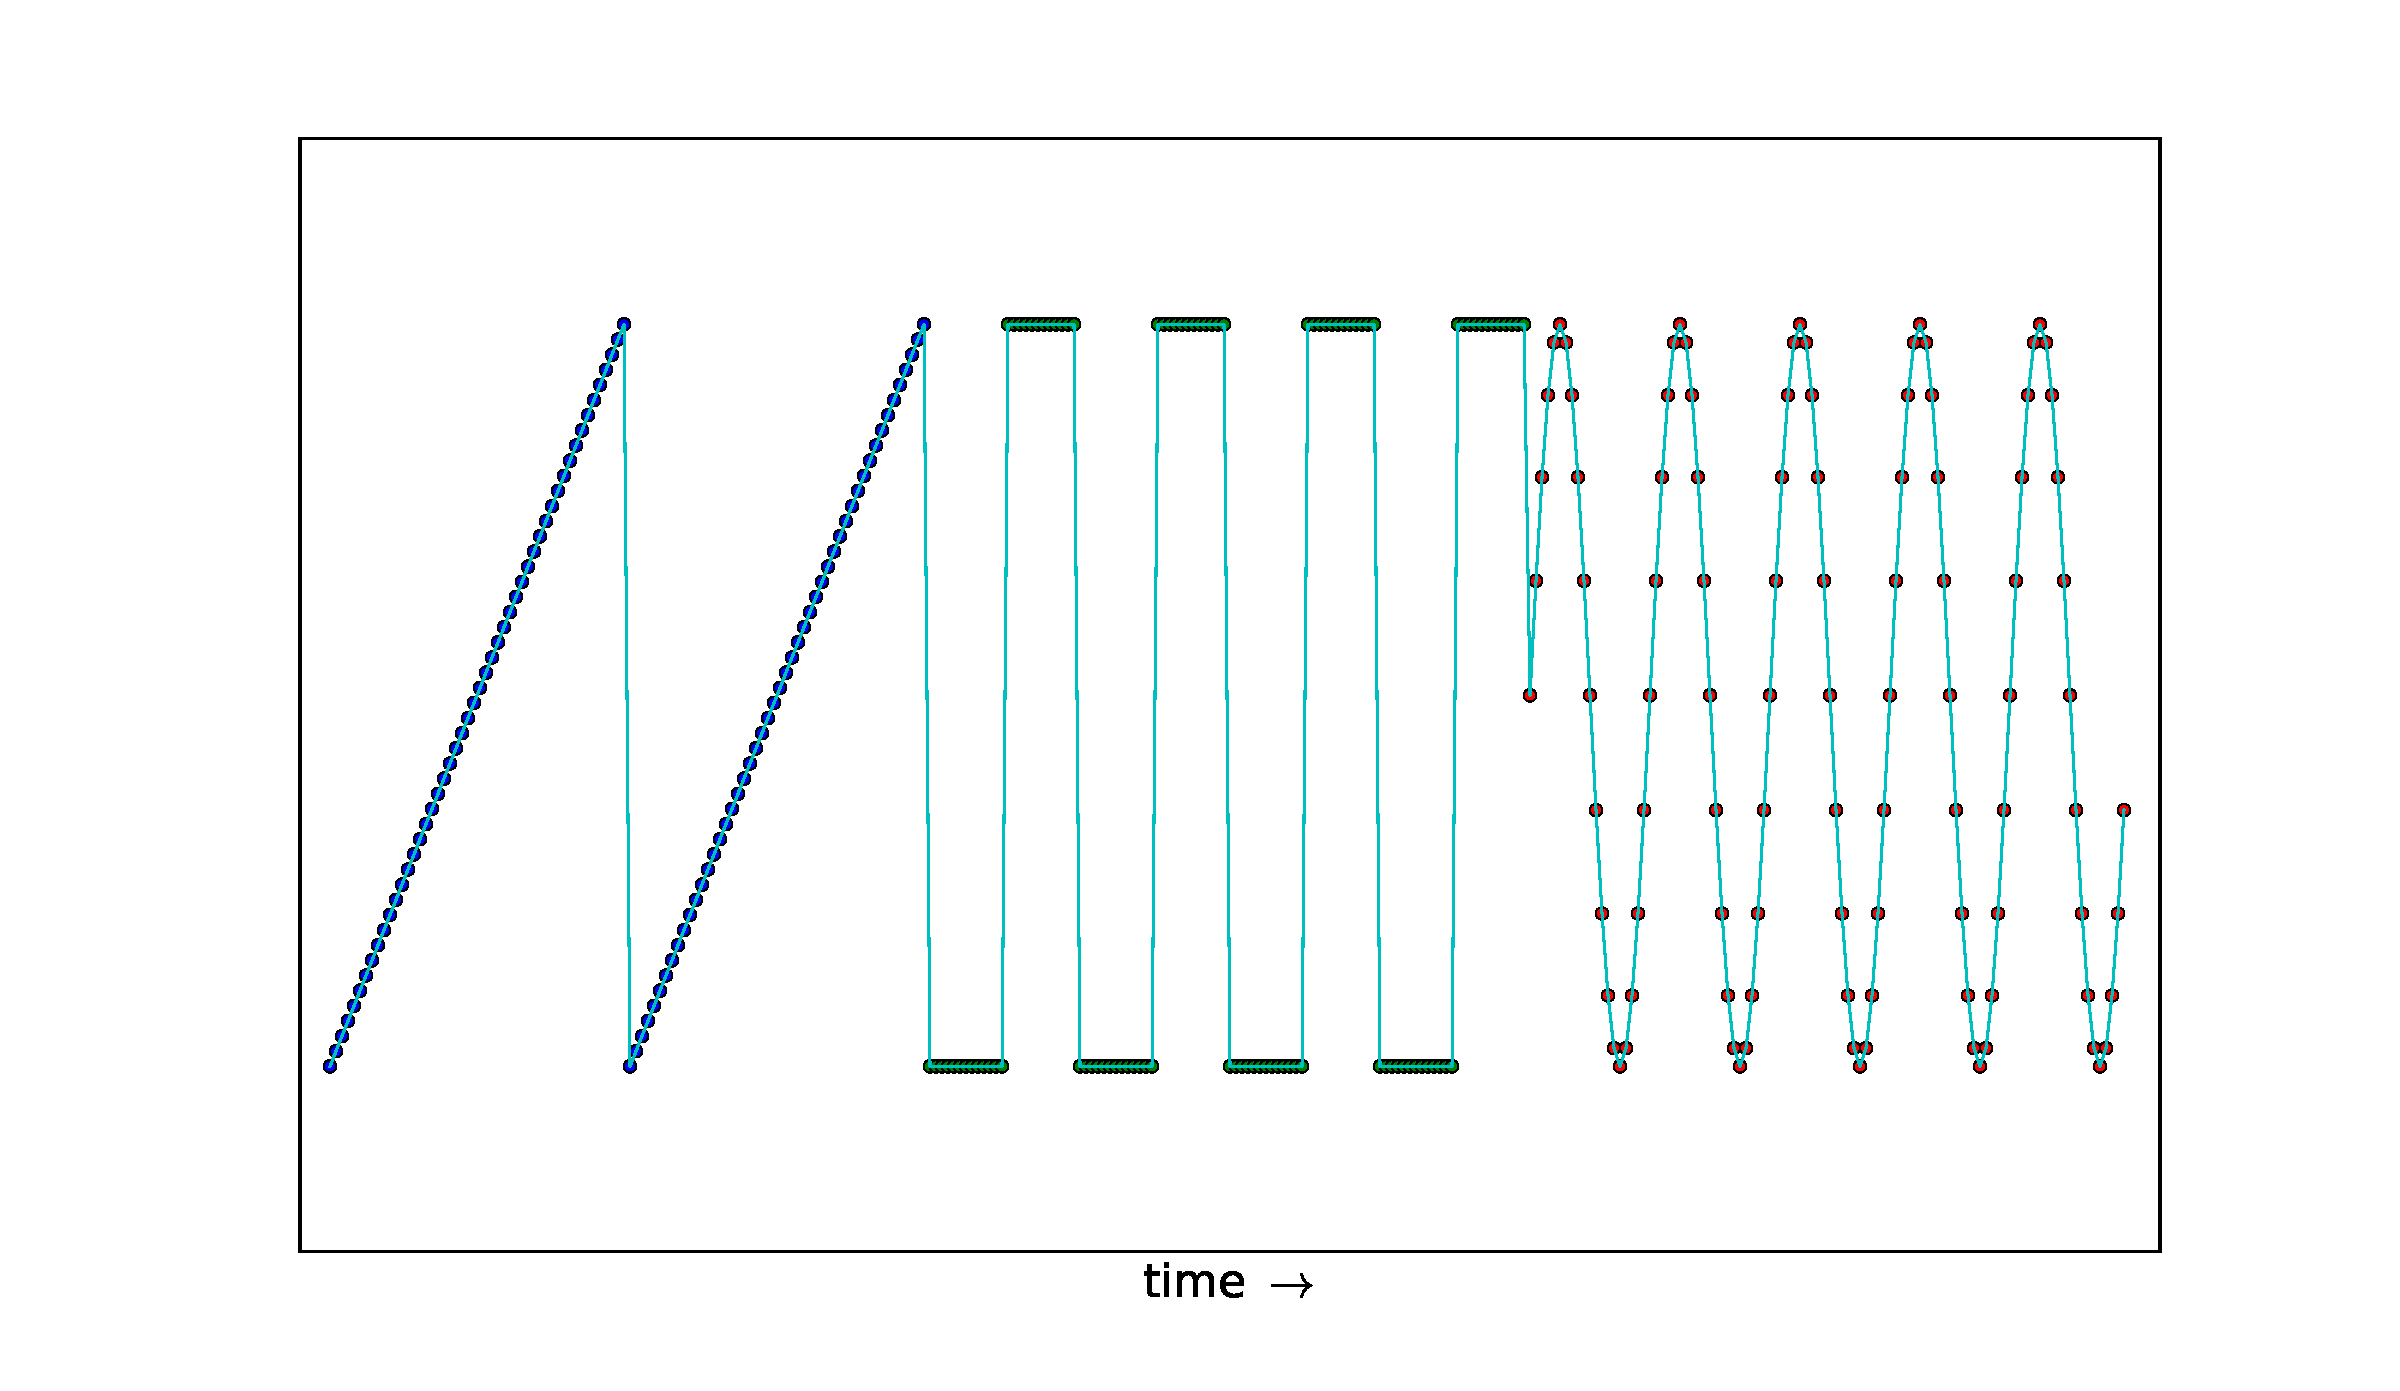
\includegraphics[width=\columnwidth]{figures/concatenacao}}
    \caption{Concatenation of three sound sequences by temporal overlap of its samples.}
        \label{fig:concatenacao}
\end{figure}

The musical piece \emph{reduced-fi} explores the temporal juxtaposition of notes, resulting in a homophobic piece. The vertical principle is demonstrated at the \emph{sounic pictures}, static sounds with peculiar spectrum. Both pieces were written in Python and are available as part of the \massa\ \emph{toolbox}.\cite{MASSA}

With the basic musical digital note carefully described, the next section develops the temporal evolution of its contents as in \emph{glissandi} and volume envelopes. Filtering of spectral components and noise generation complements the musical note as a self contained unity. Section~\ref{notasMusica} is dedicated to the organization of these notes as music by using metrics and trajectories, with regards to traditional music theory.

%%%%%%%%%%%%%%%%%%%%%%%%%%%%%%%%%%%%%%%%%%%%%%%%%%%%%%%%%%%%%%%%%%%%%%%%%%%%%
%%%%%%%%%%%%%%%%%%%%%%%%%%%%%%%%%%%%%%%%%%%%%%%%%%%%%%%%%%%%%%%%%%%%%%%%%%%%%
%%%%%%%%%%%%%%%%%%%%%%%%%%%%%%%%%%%%%%%%%%%%%%%%%%%%%%%%%%%%%%%%%%%%%%%%%%%%%


\section{Variation in the basic musical note}\label{sec:internalVar}

The basic digital music note defined in section~\ref{sec:notaDisc} has following parameters: duration, pitch, intensity (volume) and timbre. This is a useful and paradigmatic model, but does not exhaust all the aspects of a musical note.

First of all, characteristics of the note modifie along the note itself~\cite{Chowning}. For example, a 3 seconds piano note has intensity with abrupt rise at beginning and progressive decay, has spectrum variations with harmonics decaying some others that emerge along time.
These variations are not mandatory but sound synthesis guidance for musical uses, as it reflects how sounds appear in nature. This is so considered to be true, that there is a rule of thumb: to make a sound that incites interest by itself, do internal variations on it~\cite{Roederer}.
To explore all the ways in which variations occur within a note is out of the scope of any work, given the sensibility of the human ear and the complexity of human sound cognition. In the following, primary resources are presented to produce variations in the basic note. It is worthwhile to recall that all the relations in this and other sections are implemented in Python and published as the public domain \massa\ toolbox. The musical pieces \emph{Transita para metro}, \emph{Vibra e treme}, \emph{Tremolos, vibratos e a frequência}, \emph{Trenzinho de caipiras impulsivos}, \emph{Ruidosa faixa}, \emph{Bela rugosi}, \emph{Chorus infantil}, \emph{ADa e SaRa} were made to validate and illustrate concepts of this section. The code that synthesizes these pieces are also part of the toolbox\cite{MASSA}.
 
\subsection{Lookup Table}\label{subsec:lookup}

The \emph{Lookup Table} (or simply LUT), is an array for indexed operations which substitutes continuous and repetitive calculation. It is used to reduce computational complexity and to use functions without direct calculation, as data sampled from nature.
In music its usage transcends these applications, as it simplifies many operations and makes possible the use a single wave period to synthesize sounds in the whole audible spectrum, with any waveform.

\begin{figure*}
    \centering
        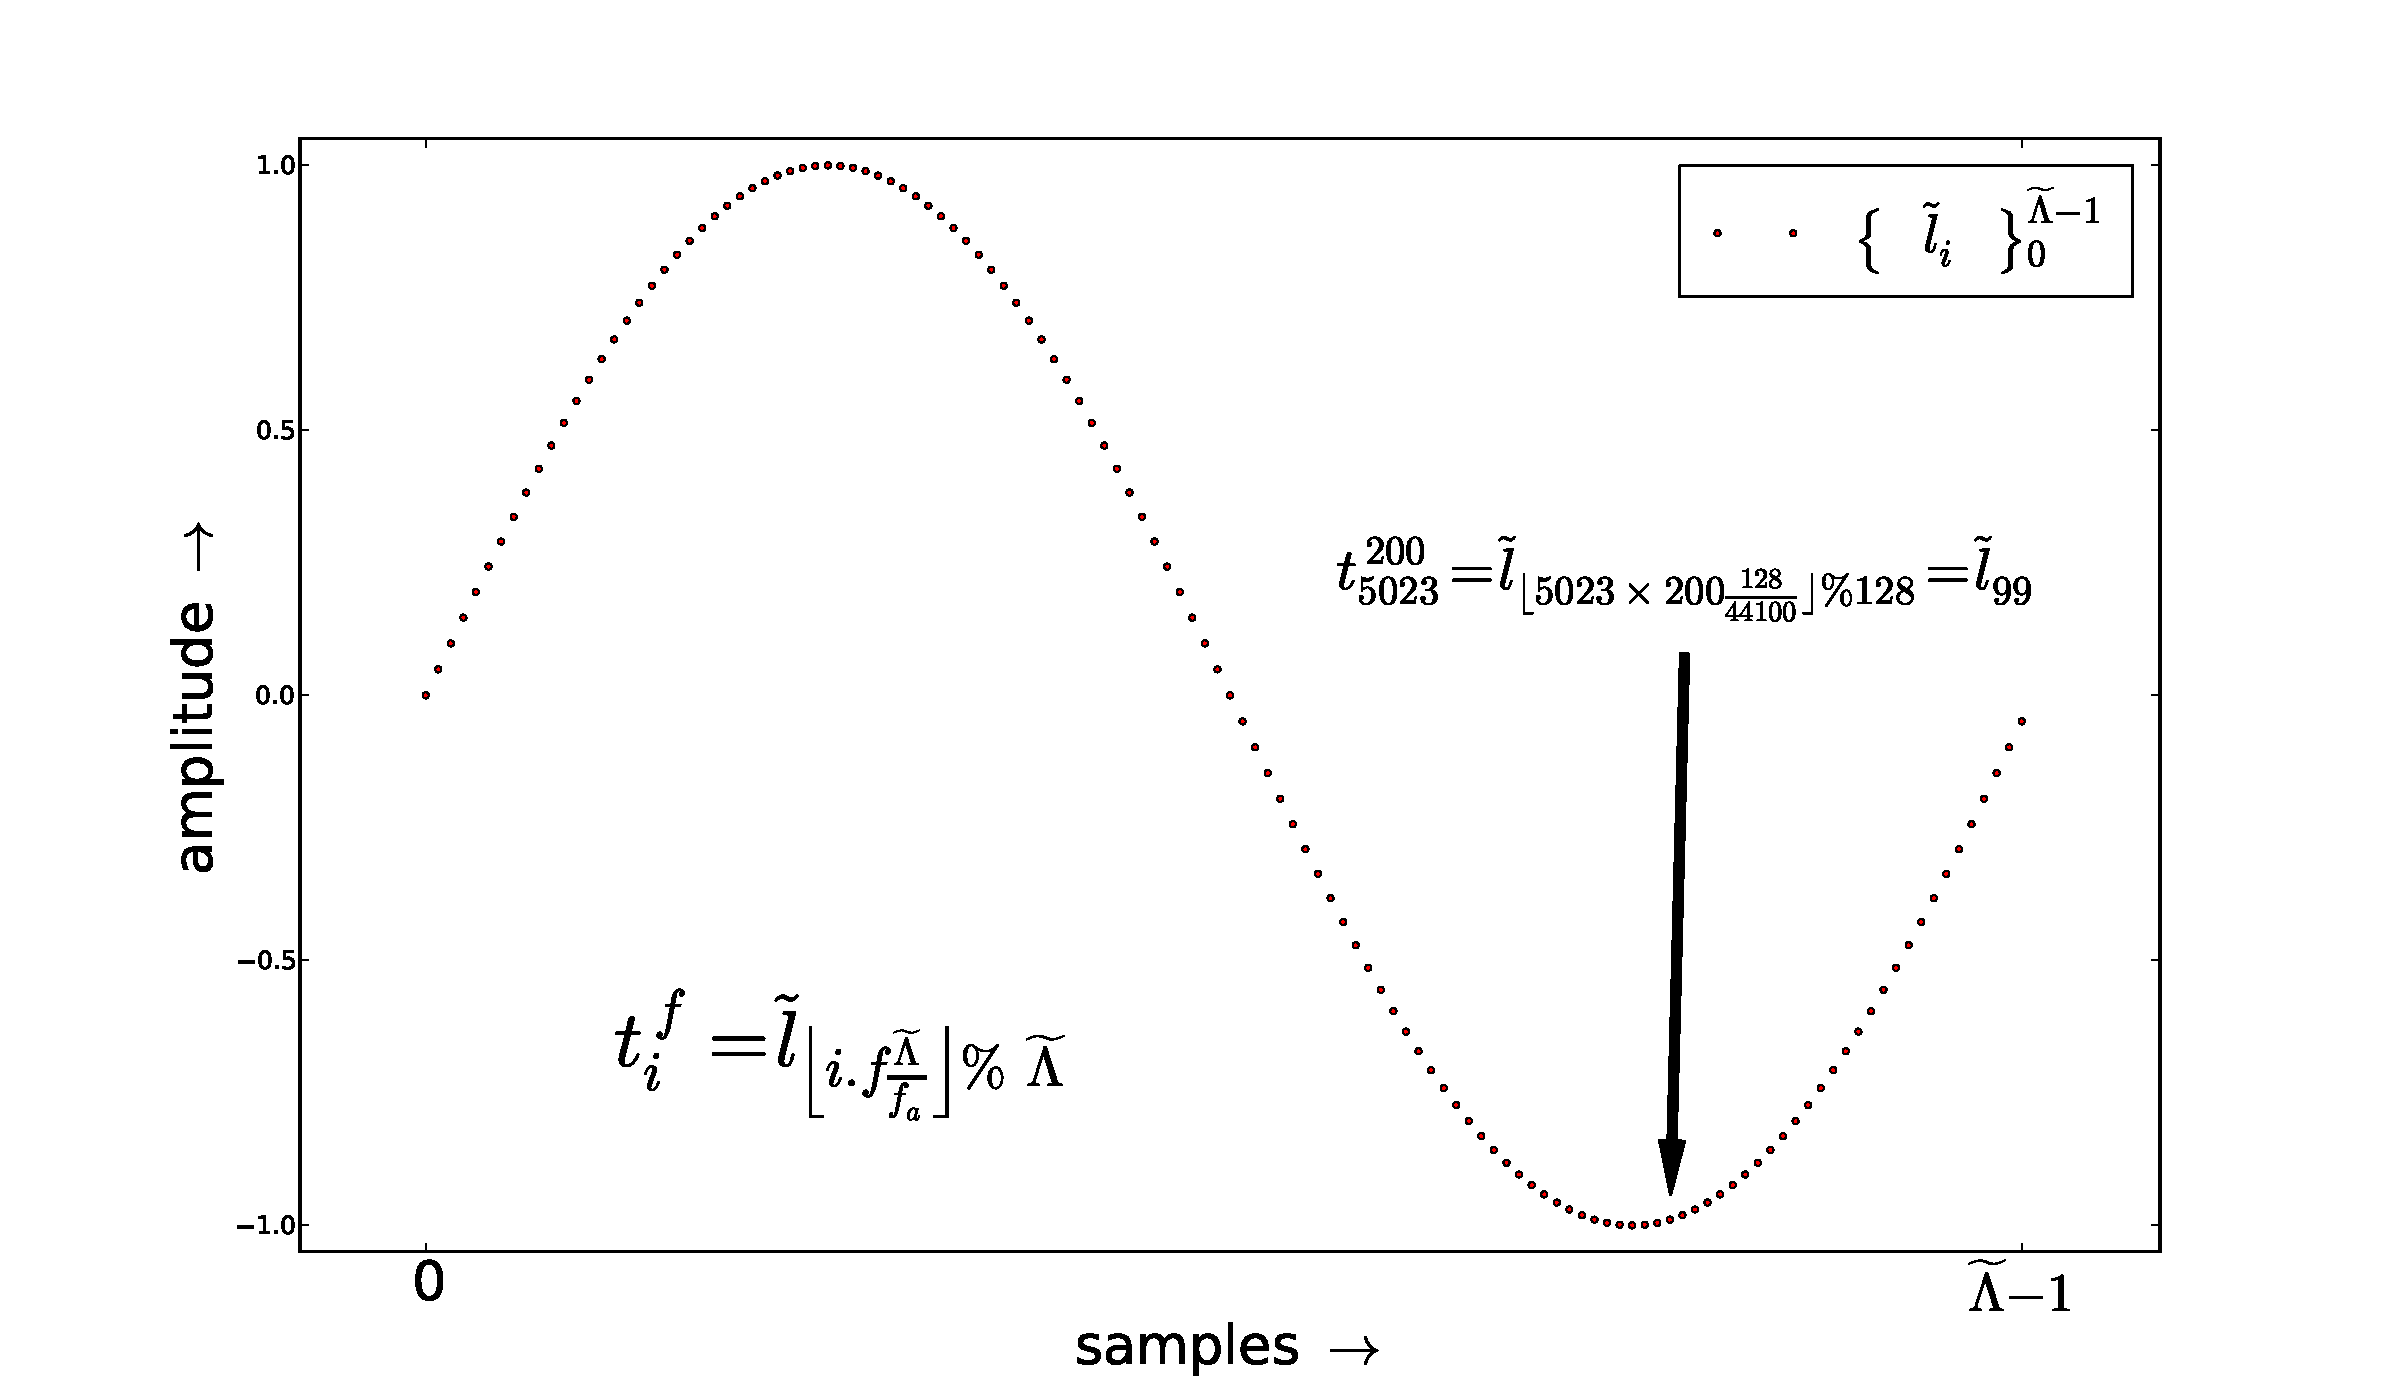
\includegraphics[width=\textwidth]{figures/lut}
    \caption{Search in the \emph{lookup table} to synthesize sounds in different frequencies using an unique waveform with high resolution.}
        \label{fig:lut}                                                                                                            
\end{figure*}

Be $\widetilde{\Lambda}$ the wave period in samples and $\widetilde{L_i} = \left\{\, \widetilde{l}_i \,\right\}_0^{\widetilde{\Lambda} -1}$ the samples $\widetilde{l_i}$ (refer to Equation~\ref{periodoUnico}), a sequence $T_i^{f,\,\Delta}$ with samples of a sound with frequency $f$ and duration $\Delta$ can be obtained by means of $\widetilde{L_i}$:

\begin{equation}\label{eq:lut}
\begin{split}
T_i^{f,\,\Delta}=\left\{t_i^f\right\}_0^{\lfloor \, f_a . \Delta \, \rfloor -1} = & \left\{ \, \widetilde{l}_{\gamma_i \% \widetilde{\Lambda} }\, \right\}_{0}^{\Lambda-1}\; , \quad \\ \text{where} \;\; \gamma_i = & \left \lfloor i . f \frac{ \widetilde{\Lambda}}{f_a} \right \rfloor  
\end{split}
\end{equation}

In other words, with the right LUT indexes ($\gamma_i\%\widetilde{\Lambda}$) it is possible to synthesize sounds at any frequency. Figure~\ref{fig:lut} illustrates the calculation of $\{t_i\}$ sample from $\left\{\,\widetilde{l}_i\,\right\}$ for $f=200Hz$, $\widetilde{\Lambda}=128$ and adopting the sample rate of $f_s=44.1kHz$.
Though this is not a practical configuration (as assigned below), it makes possible a graphical visualization of the procedure.

The calculation of the integer $\gamma_i$ introduces noise which decreases as $\widetilde{\Lambda}$ increases.
In order to use this calculation in sound synthesis, with $f_s=44.1 kHz$, the standard guidelines suggests the use of $\widetilde{\Lambda} = 1024$ samples, since it does not produce relevant noise on the audible spectrum. The rounding or interpolation method are not decisive in this process~\cite{Geiger}.

The expression defining the variable $\gamma_i$ can be understood as $f_s$ being added to $i$ at each second.
If $i$ is divided by the sample frequency, $\frac{i}{f_a}$
is incremented in $1$ at each second. Multiplied by the period, it results in $i \frac{\widetilde{\Lambda}}{f_a}$, which covers the period in each second. Finally, with frequency $f$ it results in $i . f \frac{\widetilde{\Lambda}}{f_a}$ which completes $f$ periods $\widetilde{\Lambda}$ in $1$ second, i.e. the resulting sequence presents the fundamental frequency $f$.

There are important considerations here: it is possible to use practically any frequency $f$. Limits exist only in low frequencies when the size of the table  $\widetilde{\Lambda}$ is not sufficient for the sample rate $f_a$. The lookup procedure is virtually costless and replaces calculations by simple indexed searches (what is generally understood as an optimization process). Unless otherwise stated, this procedure will be used along all the text for every applicable case.
LUTs are broadly used in computational implementations for music. A classical usage of LUTs is known as \emph{Wavetable Synthesis}, which consists of many LUTs used together to generate a quasi-periodic music note~\cite{Cook,Wavetable}.

\subsection{Incremental Variations of Frequency and Intensity}\label{subsec:vars}

As stated by the Weber and Fechner~\cite{Weber-Fechner} law, the human perception has a logarithmic relation with the stimulus. In other words, the exponential progression of a stimulues is perceived as linear.
For didactic reasons, and given its use in AM and FM synthesis (subsection~\ref{subsec:tvaf}), linear variation is discussed first.

Consider a note with duration $\Delta = \frac{\Lambda}{f_a}$, in which the frequency $f=f_i$ varies linearly from $f_0$ to $f_{\Lambda -1}$. Thus:

\begin{equation}\label{freqLinear}
 F_i=\{f_i\}_0^{\Lambda-1}=\left\{f_0 + (f_{\Lambda-1}-f_0)\frac{i}{\Lambda-1} \right\}_0^{\Lambda-1}
\end{equation}

\begin{equation}\label{indiceLinear}
\begin{split}
 \Delta_{\gamma_i}=f_i\frac{\widetilde{\Lambda}}{f_a} \quad \Rightarrow \quad \gamma_i= \left \lfloor \sum_{j=0}^{i} f_j\frac{\widetilde{\Lambda}}{f_a} \right \rfloor \\
\gamma_i=  \left \lfloor \sum_{j=0}^{i} \frac{\widetilde{\Lambda}}{f_a} \left [f_0 + (f_{\Lambda-1}-f_0)\frac{j}{\Lambda-1} \right ] \right \rfloor 
\end{split}
\end{equation}

\begin{equation}\label{serieAmostralLin}
 \left\{t_i^{\;\overline{f_0,\, f_{\Lambda-1}}}\right\}_0^{\Lambda-1}=\left\{\,\widetilde{l}_{\gamma_i \% \widetilde{\Lambda}}\,\right\}_0^{\Lambda-1}
\end{equation}

where $\Delta_{\gamma_i}=f_i\frac{\widetilde{\Lambda}}{f_a}$ is the LUT increment between two samples given the sound frequency of the first sample.
Therefore, it is handy to calculate the elements $t_i^{\;\overline{f_0,f_{\Lambda-1}}}$ by means of the period $\left\{\widetilde{l}_i\right\}_0^{\Lambda-1}$.

The equations~\ref{freqLinear},~\ref{indiceLinear} and~\ref{serieAmostralLin} are related with the linear progression of the frequency. As stated above, the frequency progression \emph{perceived} as linear follows an exponential progression, i.e. a geometric progression of frequency is perceived as an arithmetic progression of pitch.
It is possible to write: $f_i=f_0 . 2^{\frac{i}{\Lambda-1} n_8}$ where  $n_8=\log_2\frac{f_{\Lambda-1}}{f_0}$ is the number of octaves between $f_0$ and $f_{\Lambda-1}$.
Therefore, $f_i=f_0 . 2^{\frac{i}{\Lambda-1}\log_2\frac{f_{\Lambda-1}}{f_0}}=
 f_0 . 2^{\log_2\left ( \frac{f_{\Lambda-1}}{f_0} \right )^{\frac{i}{\Lambda-1}}}=
 f_0 \left ( \frac{f_{\Lambda-1}}{f_0} \right ) ^{\frac{i}{\Lambda -1}}$. Accordingly, the equations for linear pitch transition are:

\begin{equation}\label{freqExponencial}
 F_i=\{f_i\}_0^{\Lambda-1}=  \left\{f_0 \left ( \frac{f_{\Lambda-1}}{f_0} \right ) ^{\frac{i}{\Lambda -1}} \right\}_0^{\Lambda-1}
\end{equation}

\begin{equation}\label{indiceExponencial}
\begin{split}
 \Delta_{\gamma_i}= f_i\frac{\widetilde{\Lambda}}{f_a} \quad \Rightarrow  \quad \gamma_i= & \left \lfloor \sum_{j=0}^{i} f_j\frac{\widetilde{\Lambda}}{f_a} \right \rfloor \\ \gamma_i = & \left \lfloor \sum_{j=0}^{i} f_0 \frac{\widetilde{\Lambda}}{f_a} \left ( \frac{f_{\Lambda-1}}{f_0} \right ) ^{\frac{j}{\Lambda -1}} \right \rfloor
\end{split}
\end{equation}

\begin{equation}\label{serieAmostralLog}
 \left\{t_i^{\;\overline{f_0,\,f_{\Lambda-1}}}\right\}_0^{\Lambda-1}=\left\{\,\widetilde{l}_{\gamma_i \% \widetilde{\Lambda}}\,\right\}_0^{\Lambda-1}
\end{equation}

\begin{figure}[h!]
     \centering
         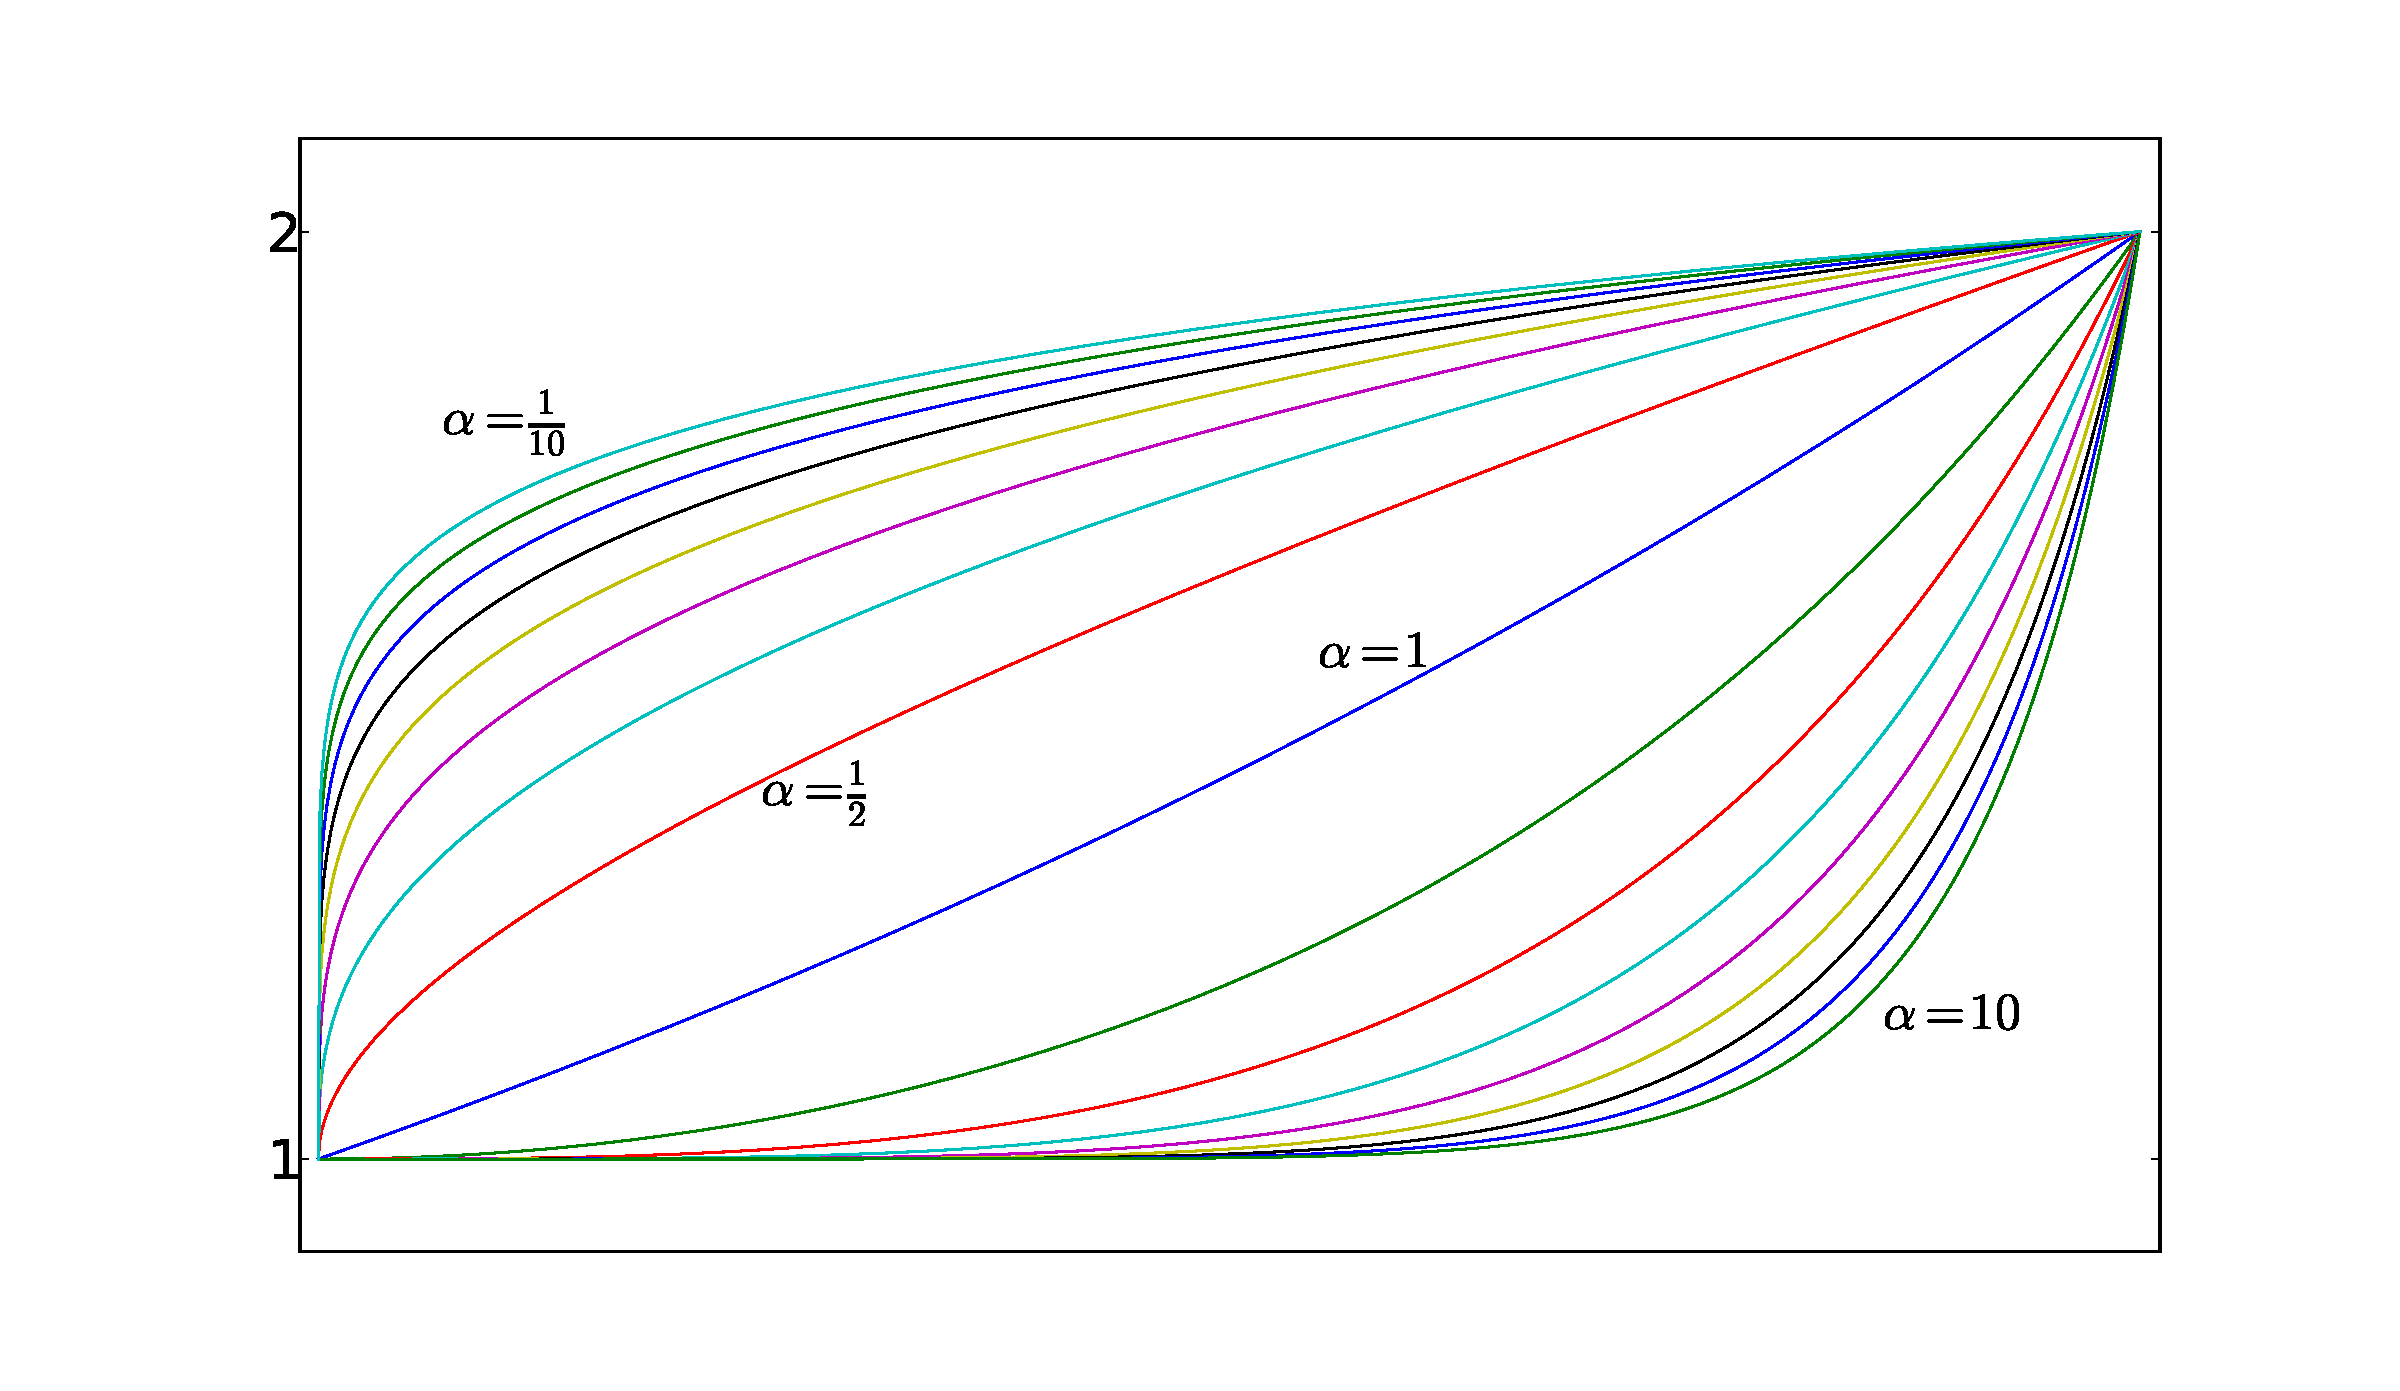
\includegraphics[width=\columnwidth]{figures/transicao}
     \caption{Intensity transitions to different values of $\alpha$ (see equations~\ref{seqAmp} and ~\ref{transAmp}).}
         \label{fig:transicao}
\end{figure}

The term $\frac{i}{\Lambda-1}$ convers the interval $[0,1]$ and it is possible to power it to a value in such a way that the beginning of the transition will be smoother or steeper.
This procedure is useful for energy variations with the purpose of changing the volume\footnote{The volume (psychophysical quality) is consequence of different sound characteristics, like reverberation and concentration of high harmonics, among which is wave total energy. Wave energy is the easy to modify (see Equation~\ref{eq:potencia}) and it can vary in many ways. The simplest way consists of modifying the amplitude by multiplying the whole sequence by a real number. The increase of energy without amplitude variation is the \emph{sound compression}, quite popular nowadays for music production~\cite{guillaume}}. It is sufficient to multiply the original sequence by the sequence $a_{\Lambda-1}^{\left( \frac{i}{\Lambda-1} \right )^\alpha}$, where $\alpha$ is the given coefficient and $a_{\Lambda-1}$ is a fraction of the original amplitude, which is the value to be reached at the end of transition.

Thus, for amplitude variations:

\begin{equation}\label{seqAmp}
\begin{split}
 \{a_i\}_0^{\Lambda-1}= & \left \{ a_0 \left ( \frac{a_{\Lambda-1}}{a_0} \right )^{\left ( \frac{i}{\Lambda-1} \right )^\alpha} \right \}_0^{\Lambda-1}= \\ = & \left \{ \left ( {a_{\Lambda-1}} \right )^{\left ( \frac{i}{\Lambda-1} \right )^\alpha} \right \}_0^{\Lambda-1} \text{ (with } a_0=1 \text{)}
\end{split}
\end{equation}
and
\begin{equation}\label{transAmp}
\begin{split}
 T_i^{'}=T_i \odot A_i = & \{t_i . a_i\}_0^{\Lambda-1} \\ = & \left \{ t_i . (a_{\Lambda-1} )^{\left ( \frac{i}{\Lambda-1} \right )^\alpha} \right \}_0^{\Lambda-1}
\end{split}
\end{equation}

It is often convenient to have $a_0=1$ in order to start a new sequence with the original amplitude and then progressively change it.
If $\alpha=1$, the amplitude variation follows the geometric progression whose defines the linear variation of volume. Figure~\ref{fig:transicao} depicts transitions between values 1 and 2 and for different values of $\alpha$, a gain of $\approx 6dB$ as given by equation~\ref{eq:ampVol}.

Special attention should be dedicated while considering $a=0$.
In equation~\ref{seqAmp}, $a_0=0$ results in a division by zero and if $a_{\Lambda-1}=0$, there will be multiplication by zero. Both cases make the procedure useless, once no number different from zero can be represented as a ratio in relation of zero. It is possible to solve this dilemma choosing a number that is small enough like $-80dB\;\Rightarrow a=10^{\frac{-80}{20}}=10^{-4}$ as the minimum volume for a \emph{fade in} ($a_0=10^{-4}$) or for a \emph{fade out} ($a_{\Lambda-1}=10^{-4}$). A linear fade can be used to reach zero amplitude. Another common solution is the use of the quartic polynomial term $x^4$, as it reaches zero without these difficulties and gets reasonably close to the curve with $\alpha=1$ as it withdraws from zero~\cite{Cook}.

For linear amplification -- but not linear perception -- it is sufficient to use an appropriate sequence $\{a_i\}$:

\begin{equation}\label{seqAmpLin}
a_i=a_0 + (a_{\Lambda-1}-a_0)\frac{i}{\Lambda-1}
\end{equation}

Here the convertion between decibels and amplitude is convenient. In this way, the equations~\ref{ampDec} and \ref{transAmp} specify a transition of $V_{dB}$ decibels:

\begin{equation}\label{seqAmpDB}
T_i^{'}=\left\{ t_i 10^{\frac{V_{dB}}{20}\left( \frac{i}{\Lambda-1} \right)^\alpha} \right\}_0^{\Lambda-1}
\end{equation}

\noindent for the general case of amplitude variations following a geometric progression. The greater the value of $\alpha$, the smoother the sound introduction and more intense its end. $\alpha>1$ results in volume transitions commonly called \emph{slow fade}, while $\alpha<1$ results in \emph{fast fade}\cite{guillaume}.

The linear transitions will be used for AM and FM synthesis, while logarithmic transitions are proper tremolos and vibratos, as developed in subsection~\ref{subsec:tvaf}. A non-oscillatory exploration of these variations is in the music piece \emph{Transita para metro}, which code is online as part of the \massa\ toolbox\cite{MASSA}.


\subsection{Application of Digital Filters}\label{subsec:filtros}

This subsection is limited to a description of sequences processing, by convolution and differential equations, and immediate applications, as its complexity escapes the scope of this study\footnote{The implementation of filters comprehends an area of recognized complexity, with dedicated literature and software implementations. The reader is welcome to visit the bibliography for further discussion~\cite{Openheim,smith}.}. Filter applications can be part of the synthesis process or made subsequently as part of processes commonly called ``sound treatment''.
\subsubsection{Convolution and finite impulse response (FIR) filters}

\begin{figure*}
     \centering
         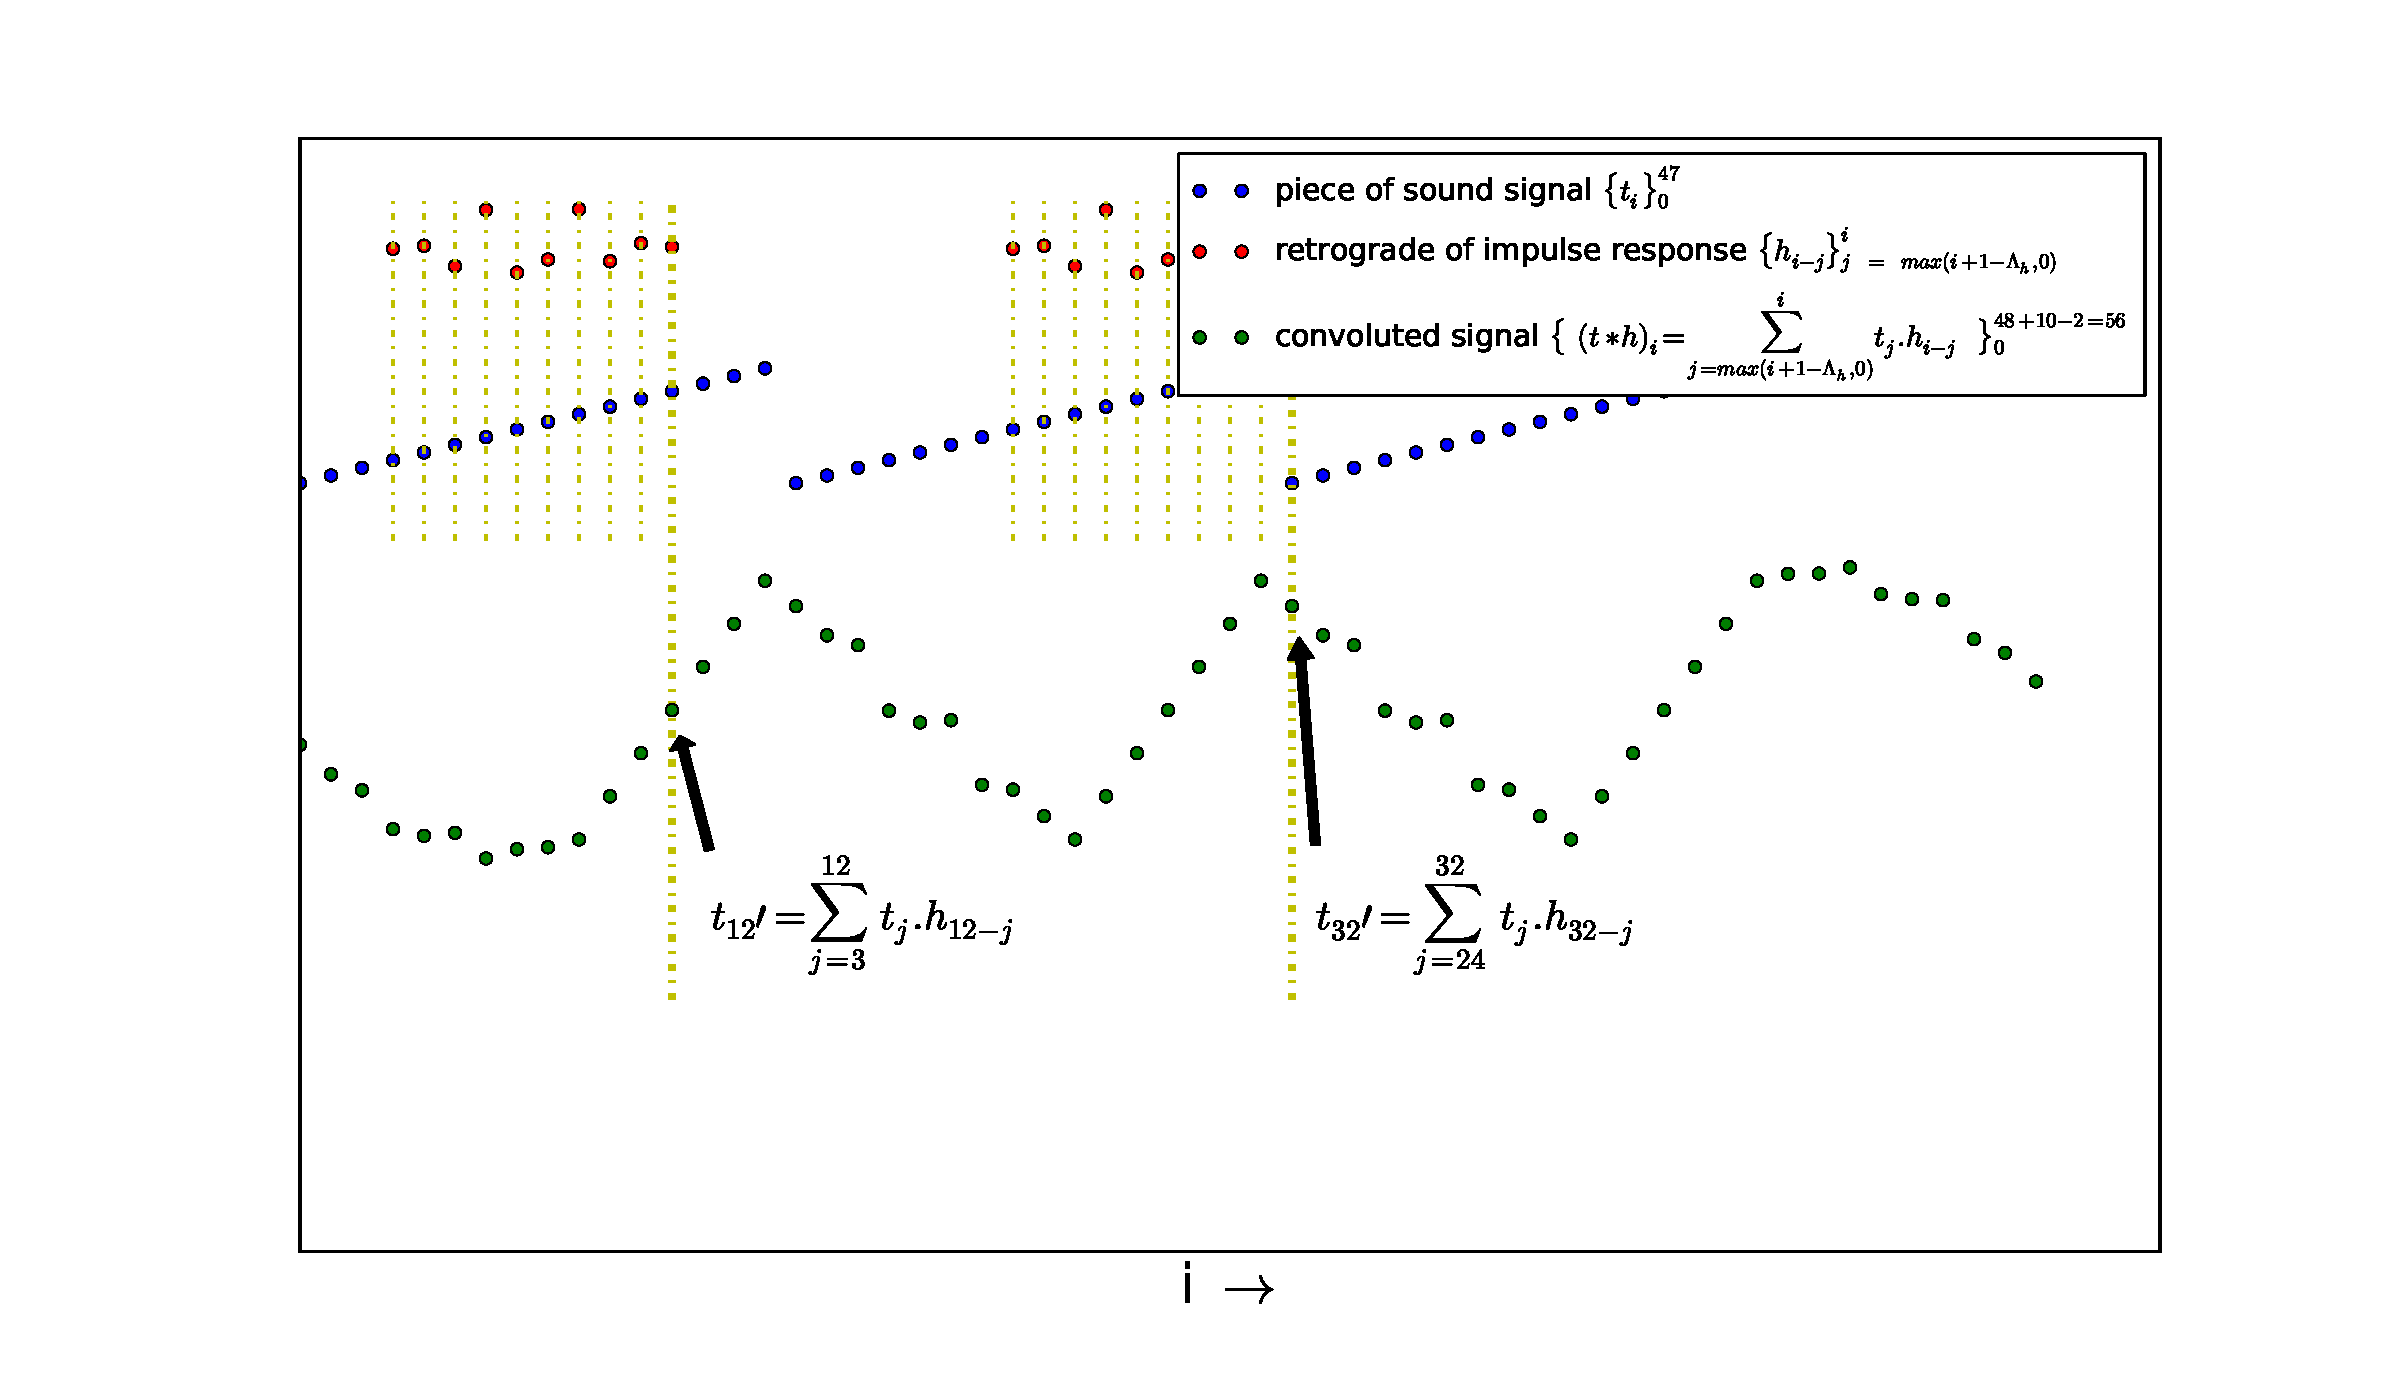
\includegraphics[width=\textwidth]{figures/convolucao}
     \caption{Graphical interpretation of convolution. Each resulting sample is the sum of the previous samples of a signal, with each one multiplied by the retrograde of the other sequence.}
         \label{fig:conv}
\end{figure*}

Filters applied by means of convolution are known by the acronym FIR (Finite Impulse Response) and are characterized by having a finite sample representation. This sample representation is called `impulse response' $\{h_i\}$. FIR filters are applied in the time domain of digital sound by means of convolution with the respective impulse response of the filter\footnote{It is possible to apply the filter in the frequency domain multiplying the Fourier coefficients of both sound and the impulse response, and then performing the inverse Fourier transform in the resulting spectrum.\cite{Openheim}}. For the purposes of this work, the convolution is defined as:

\begin{equation}\label{eq:conv}
 \begin{split}
 \left\{t_i'\right\}_0^{\Lambda_t+\Lambda_h-2\; = \;\Lambda_{t\, '}-1} = & \{(T_j*H_j)_i\}_0^{\Lambda_{t \, '}-1} \\ = & \left \{ \sum_{j=0}^{min(\Lambda_h-1,i)}h_{j} t_{i-j} \right \}_0^{\Lambda_{t\, '}-1} 
     \\ = & \left \{ \sum_{j=max(i+1-\Lambda_h,0)}^{i}t_j h_{i-j} \right \}_0^{\Lambda_{t\, '}-1}
 \end{split}
\end{equation}

\noindent where $t_i=0$ for the samples not given.
In other words, the sound $\{t_i'\}$, resulting from the convolution of $\{t_i\}$, with the impulse response $\{h_i\}$, has each $i$-th sample $t_i$ overwritten by the sum of its last $\Lambda_h$ samples $\{t_{i-j}\}_{j=0}^{\Lambda_h-1}$ multiplied one-by-one by samples of the impulse response $\{h_i\}_0^{\Lambda_h-1}$. This procedure is illustrated in Figure~\ref{fig:conv}, where the impulse response $\{h_i\}$ is in its retrograde form, and $t_{12}'$ and $t_{32}'$ are two calculated samples using the convolution given by $(T_j*H_j)_i=t_i'$. The final signal always has the length of $\Lambda_t+\Lambda_h -1=\Lambda_{t'}$.

With this procedure it is possible to apply reverberators, equalizers, \emph{delays}, to name a few of a variety of other filters for sound processing and to obtain musical/artistic effects.

The impulse response can be provided by physical measures or by pure synthesis. An impulse response for a reverberation application, for example, can be obtained by sound recording of the environment when someone triggers a snap which resembles an impulse, or obtained by a sinusoidal sweep whose Fourier transform approximates its frequency response. Both are impulse responses which, properly convoluted with the sound sequence, result in the own sound with a reverberation that resembles the original environment where the measure was made~\cite{Cook}.

The inverse Fourier transform of an even and real envelope is an impulse response of a FIR filter. Convoluted with a sound, it performs the frequency filtering specified by the envelope. The greater the number of samples, the higher the envelope resolution and the computational complexity, which should often be weighted, for the convolution is expensive.

An important property is the time shift caused by convolution with a shifted impulse. Despite computationally expensive, it is possible to create \emph{delay lines} by means of sound convolution with an impulse response that has an impulse for each reincidence of the sound.
In figure~\ref{fig:delays} it is possible to observe the shift caused by convolution with an impulse. Depending on the intensity of the impulses, the result is perceived as rhythm (from an impulse for each couple of seconds to about 20 impulses per second) or as pitch (from about 20 impulses per second and higher frequencies). In the latter case, the process resembles granular synthesis, reverbs and equalization.

\begin{figure*}
    \centering
        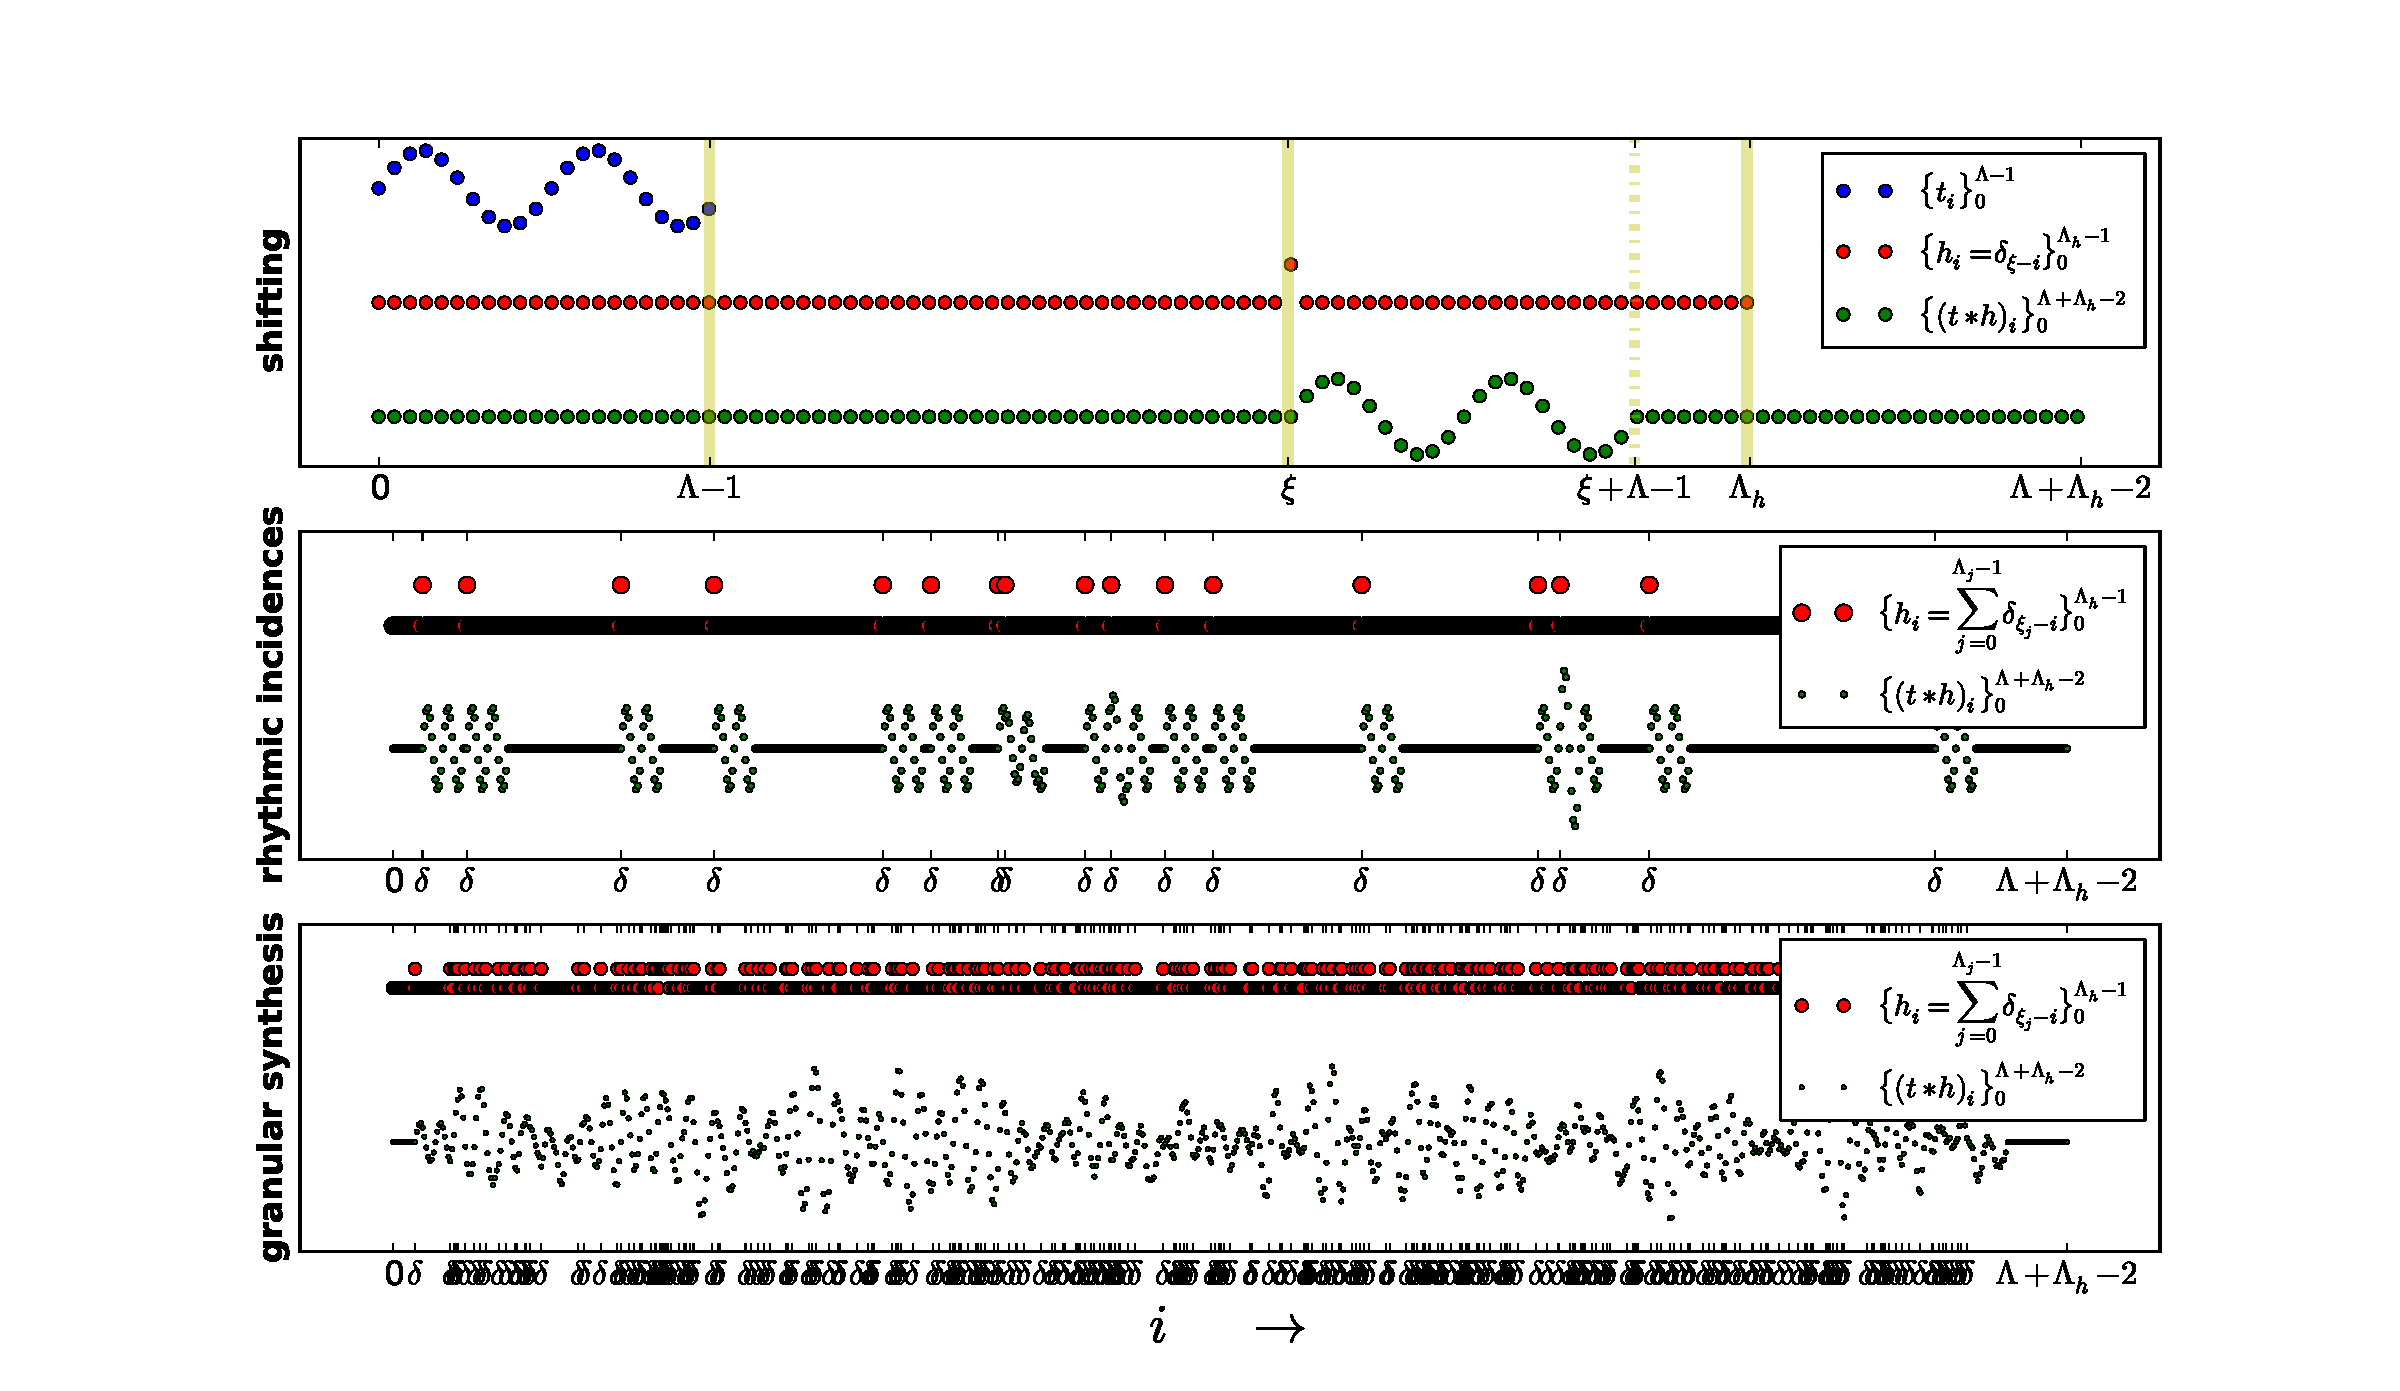
\includegraphics[width=\textwidth]{figures/delays}
    \caption{Convolution with the impulse: shifting (a), delay lines (b) and granular synthesis~(c). Disposed in increasing order of its pulse density.}
        \label{fig:delays}
\end{figure*}

\subsubsection{Infinite impulse response (IIR) filters}

This class of filters, known by the acronym IIR, are characterized by having an infinite time representation, i.e.\ the impulse response does not converge to zero. Its application is usually made by the following equation:

\begin{equation}\label{eq:diferencas}
 t_i' = \frac{1}{b_0}\left ( \sum_{j=0}^Ja_j . t_{i-j} + \sum_{k=1}^Kb_k . t_{i-k}' \right )
\end{equation}

In the most cases it is possible to normalize the variables: $a_j'=\frac{a_j}{b_0}$ and $b_k'=\frac{b_k}{b_0} \Rightarrow b_0' = 1$.
Equation~\ref{eq:diferencas} is called `difference equation' because the resulting samples $\left\{t_i'\right\}$ are given by differences between original samples $\{t_i\}$ and previous resulting ones $\left\{t_{i-k}'\right\}$.

There are many methods and tools to obtain IIR filters. The text bellow lists a selection of them for didactic purposes and as a reference. They are well behaved filters whose aspects are described in figure~\ref{fig:iir}.

For filters of simple order, the cutoff frequency $f_c$ is where the filter performs an attenuation of $-3dB \approx 0.707 $ of the original amplitude.
For band-pass and band-reject (or 'notch') filters, this attenuation has two specifications: $f_c$ (in this case, the `center frequency') and bandwidth $bw$.
In both frequencies $f_c \pm bw$ there is an attenuation of $\approx 0.707$ of the original amplitude.
There is sound amplification in band-pass and band-reject filters when the cutoff frequency is low and the band width is large enough. In trebles, those filters present only a deviation of the expected profile, expanding the envelope to the bass.

For filters with other frequency responses, it is possible to apply them successively. Another possibility is to use a biquad 'filter receipt'\footnote{Short for 'biquadratic': its transfer function has two poles and two zeros, i.e. its first direct form consists of two quadratic polynomials forming the fraction: $\mathbb{H}(z)=\frac{a_0+a_1.z^{-1}+a_2.x^{-2}}{1- b_1.z^{-1} -b_2 . z^{-2}}$.} or the calculation of Chebichev filter coefficients\footnote{Butterworth and Elliptical filters can be considered as special cases of Chebichev filters~\cite{Openheim,smith}.}.
Both alternatives are explored by referenced studies, in special~\cite{JOSFM,smith}, and by the collection of filters maintained by the \emph{Music-DSP} community of the Columbia University~\cite{music-dsp,Openheim}.

\begin{figure*}
    \centering
        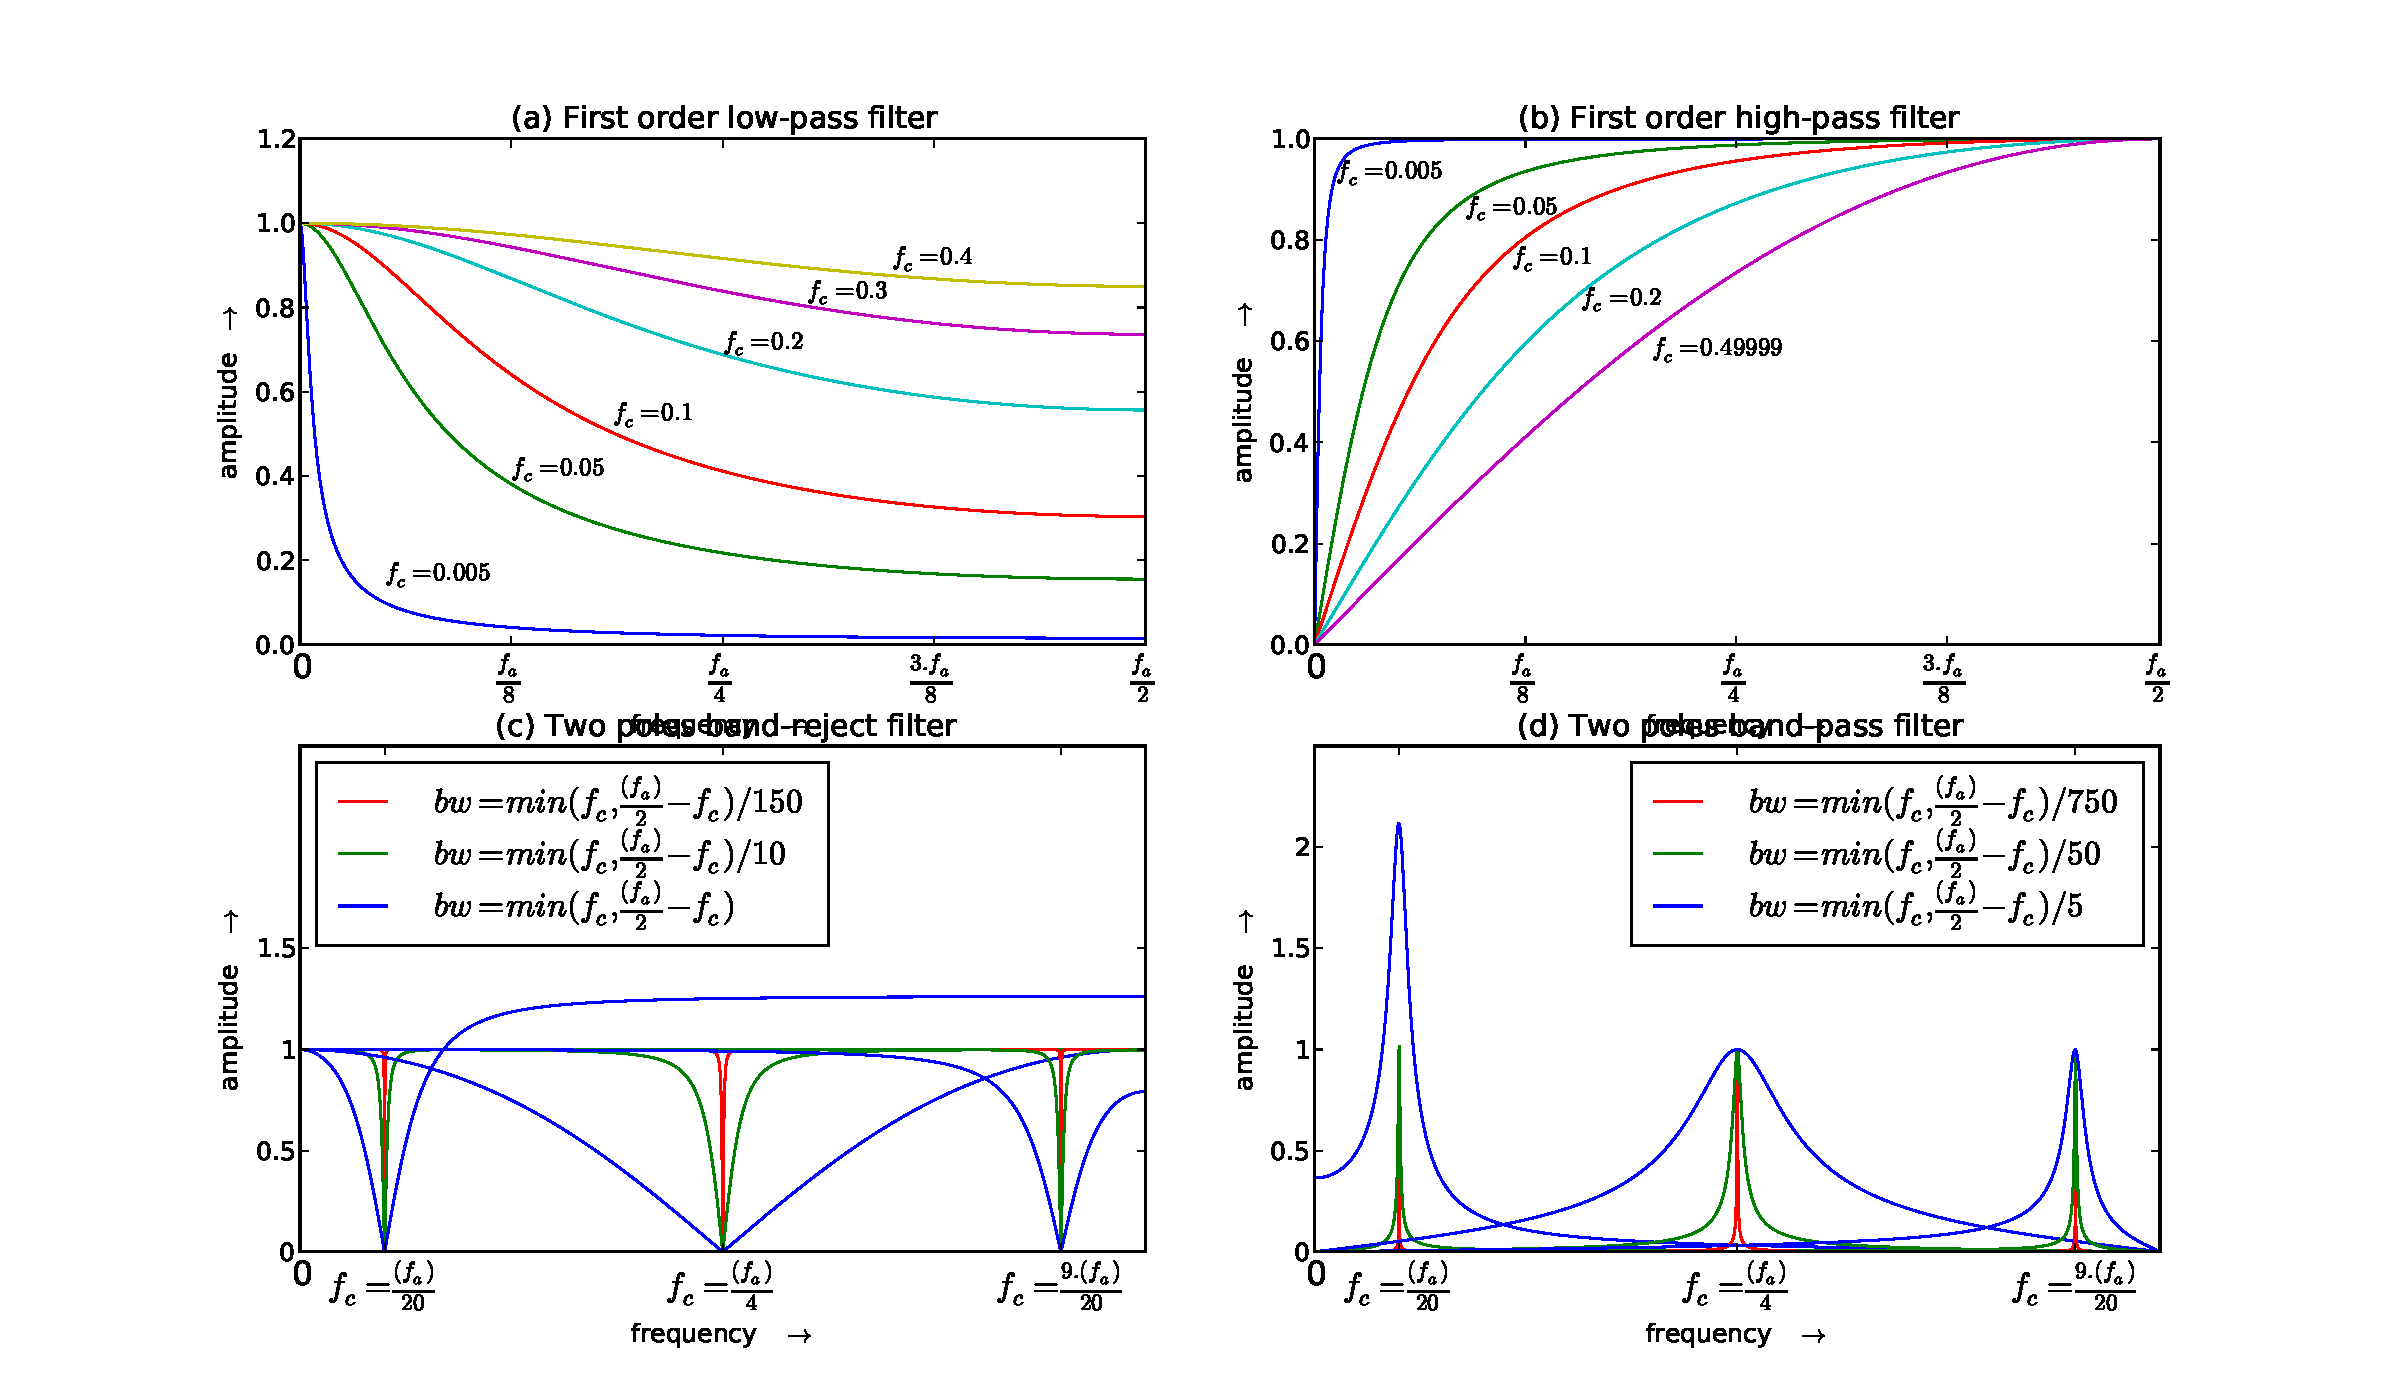
\includegraphics[width=\textwidth]{figures/iir}
    \caption{Modules for the frequency response (a), (b), (c) and (d) for IIR filters of equations~\ref{eq:passa-baixas}, \ref{eq:passa-altas}, \ref{eq:passa-banda} and \ref{eq:rejeita-banda} respectively, considering different cutoff frequencies, center frequencies and band width.}
        \label{fig:iir}
\end{figure*}


\begin{enumerate}
  \item Low-pass with a simple pole, module of the frequency response in the upper left corner of figure~\ref{fig:iir}. The general equation has the cutoff frequency $f_c \in (0,\frac{1}{2})$, fraction of the sample frequency $f_s$ in which occurs an attenuation of $3dB$.
  The coefficients $a_0$ and $b_1$ of the IIR filter are given by means of the intermediate variable $x \in [e^{-\pi},1]$:

\begin{equation}\label{eq:passa-baixas}
 \begin{split}
 x & =e^{-2\pi f_c} \\
 a_0 & =  1-x \\
 b_1 & =  x
 \end{split}
\end{equation}

  \item High-pass filter with a simple pole,  module of its frequency responses at the upper right corner of figure~\ref{fig:iir}. The general equation with cutoff frequency $f_c \in (0,\frac{1}{2})$ is calculated by means of the intermediate variable $x \in [e^{-\pi},1]$:

\begin{equation}\label{eq:passa-altas}
 \begin{split}
 x & =e^{-2\pi f_c} \\
 a_0 & =  \frac{x+1}{2} \\
 a_1 & =  -\frac{x+1}{2} \\
 b_1 & =  x
 \end{split}
\end{equation}

%\item Passa-banda
%\item Rejeita-banda

\item Notch filter. This filter is parametrized by a center frequency $f_c$ and bandwidth $bw$, both given as fraction of $f_s$, therefore $f,\; bw \in (0,0.5)$. Both frequencies $f_c \pm bw$ has $\approx 0.707$ of the amplitude, i.e. attenuation of $3dB$.
Auxiliary variables $K$ and $R$ are defined as:

\begin{equation}\label{eq:varAux}
 \begin{split}
  R & = 1 - 3bw \\
  K & = \frac{1-2R\cos(2\pi f_c) + R^2}{2 - 2 \cos (2 \pi f_c)}
 \end{split}
\end{equation}

The band-pass filter in the lower left corner of figure~\ref{fig:iir} has the following coefficients:

\begin{equation}\label{eq:passa-banda}
 \begin{split}
 a_0 & =  1 - K \\
 a_1 & =  2(K-R)\cos (2\pi f_c) \\
 a_2 & =  R^2-K \\
 b_1 & =  2R \cos (2\pi f_c) \\
 b_2 & =  -R^2
 \end{split}
\end{equation}

The coefficients of band-reject filter, depicted in the lower right of figure~\ref{fig:iir}, are:

\begin{equation}\label{eq:rejeita-banda}
 \begin{split}
 a_0 & =  K \\
 a_1 & =  -2K\cos (2\pi f_c) \\
 a_2 & =  K \\
 b_1 & =  2R \cos (2\pi f_c) \\
 b_2 & =  -R^2
\end{split}
\end{equation}

%\item Biquad: pela especificação de uma frequência central, da qualidade
%e da intensidade do filtro, este filtro é simples e usual para áudio,
%permitindo ajustes mais finos. Diversas receitas podem ser encontradas
%na literatura, recomendamos especialmente as diferentes especificações
%em ~\ref{musicDSP} e ~\ref{dspguide}.

\end{enumerate}

\subsection{Noise}\label{subsec:ruidos}

Generally, sounds without an explicit pitch are called noise~\cite{Lacerda}.
They are important musical sounds, as noise present in piano notes, violin, etc. Besides that, the majority of percussion instruments does not exhibit an unequivocal pitch and their sounds are generally regarded as noise~\cite{Roederer}. In electronic music, including electro-acoustic and dance genres, noise has diverse uses and frequently characterizes the music style~\cite{Cook}. 

The absence of a definite pitch is due to the lack of a perceptible harmonic organization in the sinusoidal components of the sound.
Hence, there are many ways to generate noise.
The use of random values to generate the sound sequence $T_i$ is an attractive method but not outstandingly useful because it tends to produce white noise with little or no variations~\cite{Cook}.

Another way is to generate noise is by using the desired spectrum, from which it is possible to perform the inverse Fourier transform.
The spectral distribution should be done with care: if phases of components present proeminent correlation, the synthesized sound will concentrate energy in some periods of its duration.

\begin{figure*}
     \centering
         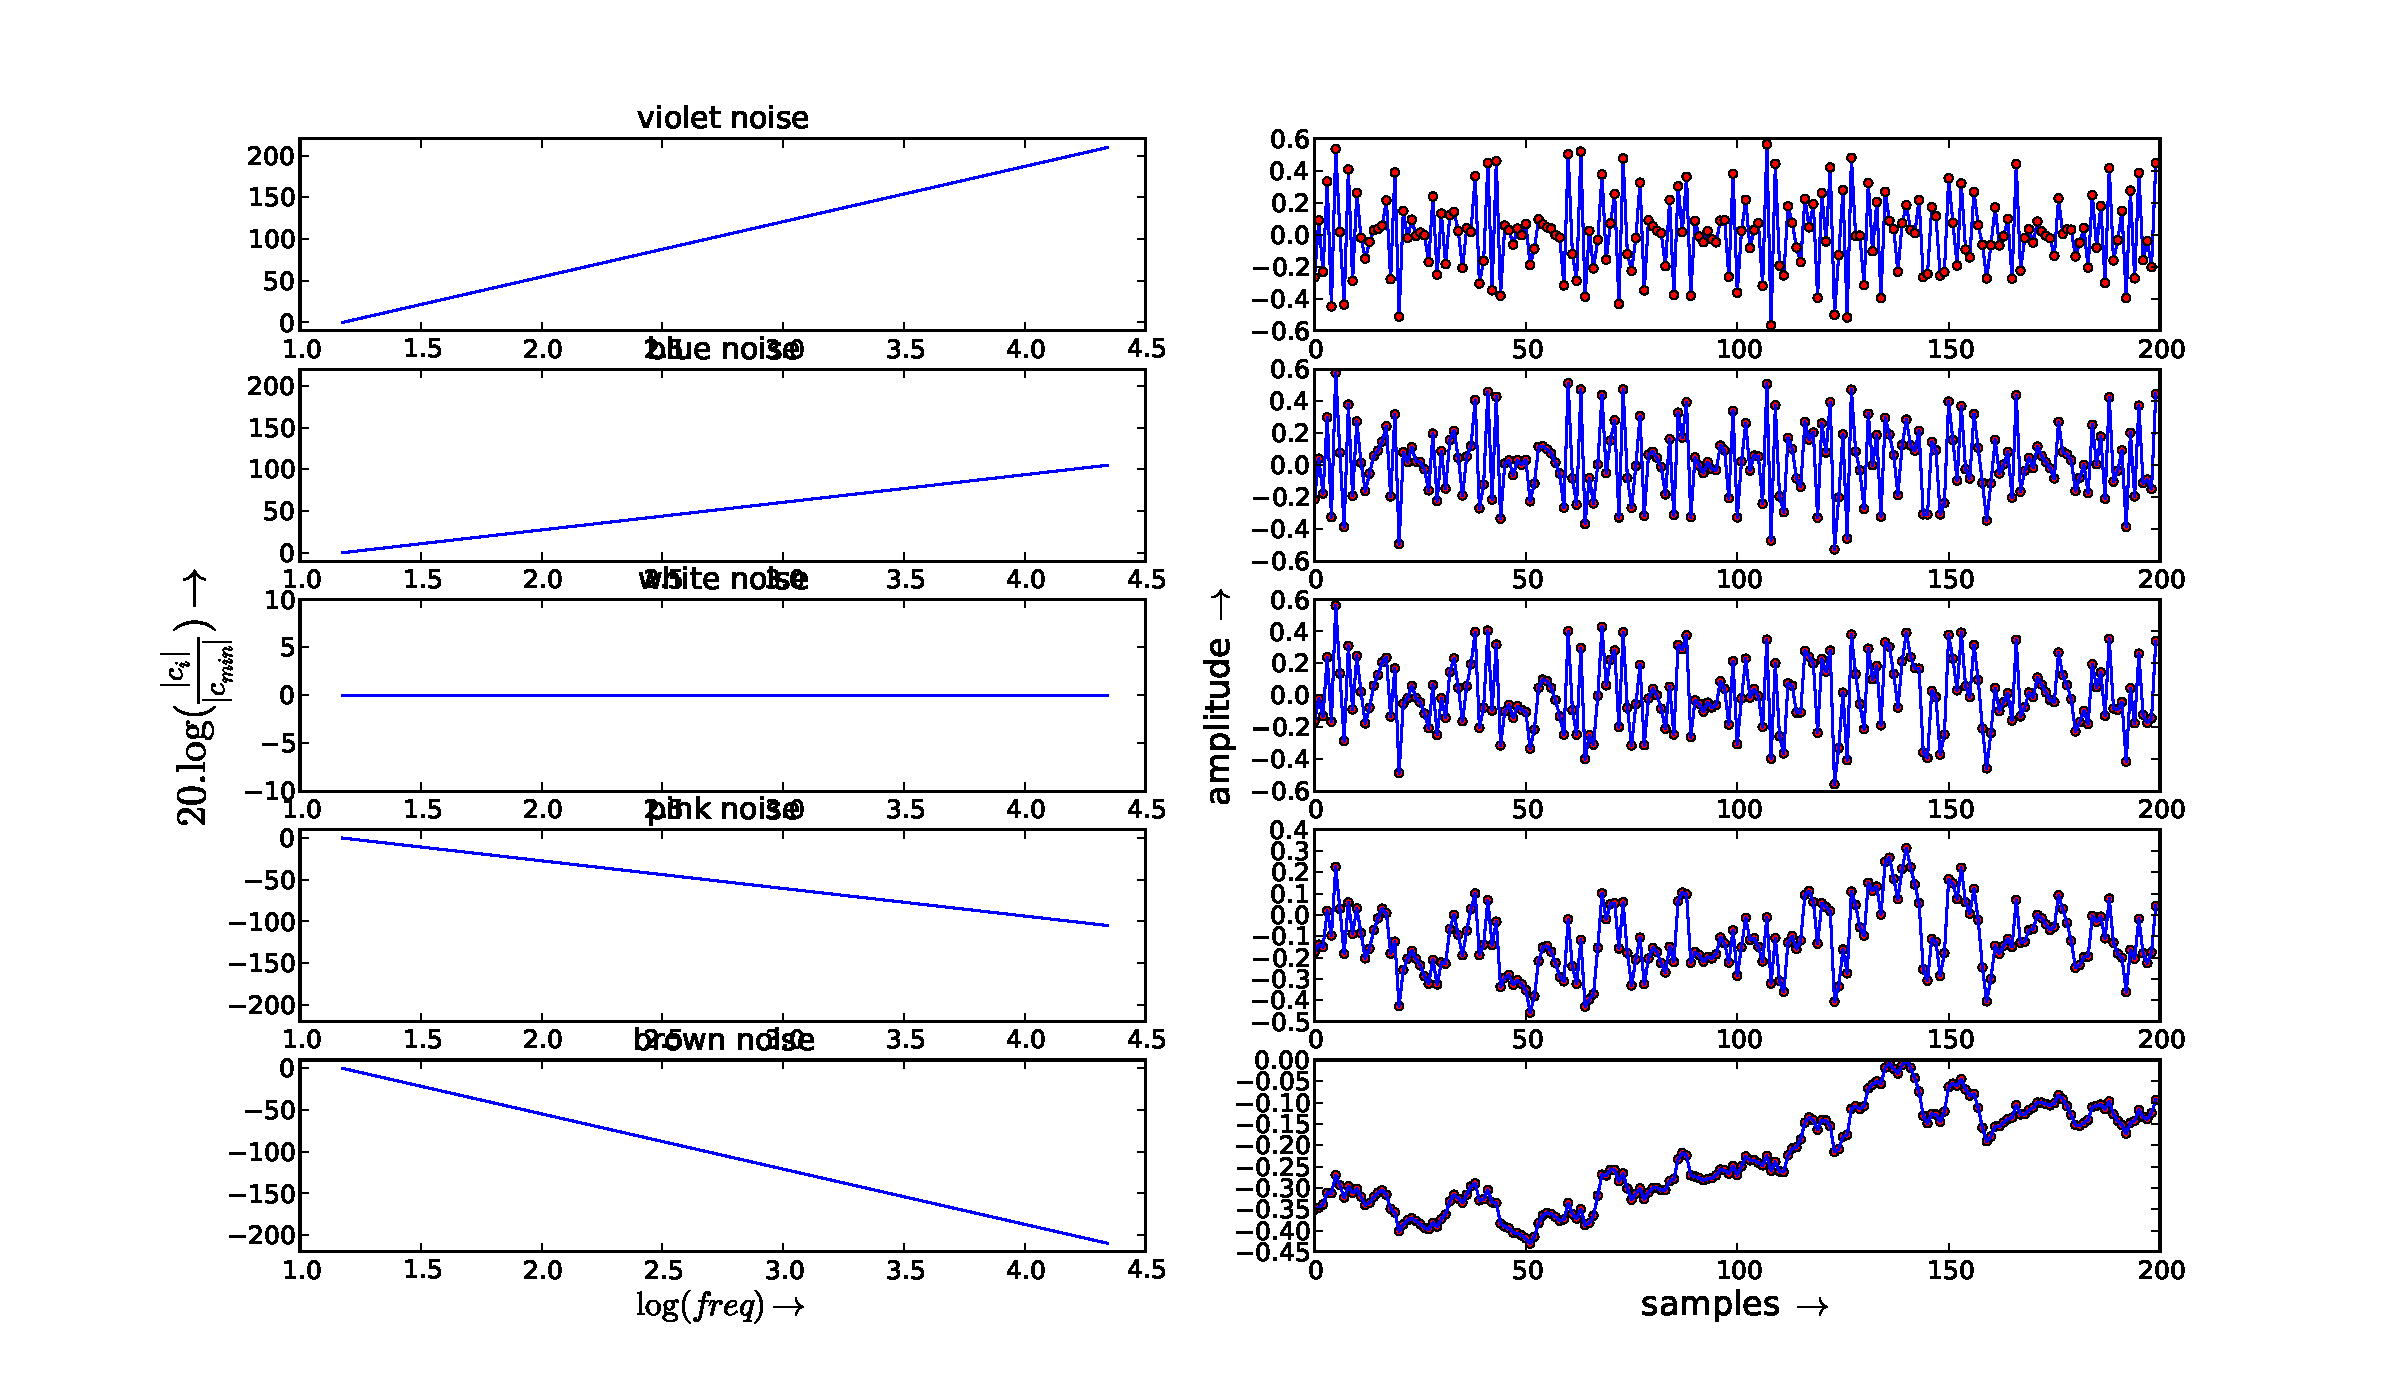
\includegraphics[width=\textwidth]{figures/ruidos}
     \caption{Colors of noise generated by equations~\ref{eq:branco}, \ref{eq:rosa}, \ref{eq:marrom}, \ref{eq:azul} and \ref{eq:violeta}: spectrum and waveforms.}
         \label{fig:ruidos}
\end{figure*}

Some noise with static spectrum are listed below. They are called \emph{colored noise} since they are associated with colors.
Figure~\ref{fig:ruidos} shows the spectrum profile and the corresponding sonic sequence side-by-side. All five noises were generated with the same phase for each component, making it possible to observe the contributions of different parts of the spectrum.

\begin{itemize}

 \item The white note has its name because its energy is distributed equally among all frequencies. It is possible to obtain white noise with the inverse transform of the following coefficients:

\begin{equation}\label{eq:branco}
 \begin{split}
 c_0 & =0 \;\text{,\quad to avoid bias} \\
 c_i & =e^{j.x}\;,\; x \; \text{random} \; \in \; [0,2\pi]\;,\; i \; \in \; \left[1, \, \frac{\Lambda}{2}-1\right] \\
 c_{\Lambda/2} & = 1 \; \text{, \; if $\Lambda$ even}\\ 
 c_i & = c_{\Lambda - i}^*\;,\;\; \text{for}\;  i \; > \;  \frac{\Lambda}{2}
 \end{split}
\end{equation}

The exponential $e^{j.x}$, is an artifice to obtain unitary module and random phase for the value of $c_i$. Besides that, $c_{\Lambda/2}$ is always real (as discussed in the previous section).

 \item The pink noise is charachterized by a decrease of $3dB$ per octave. This noise is useful for testing electronic devices, and it has prominent presence in nature~\cite{Roederer}. 

\begin{multline}\label{eq:rosa}
 %\begin{split}
 \qquad \qquad \qquad f_{\text{min}}  \approx 15 Hz \\
 f_i  = i \frac{f_a}{\Lambda} \;, \;\; \quad i \;\leq\; \frac{\Lambda}{2},\;\; i\;\in\;\mathbb{N}  \\
 \alpha_i  = \left(10^{-\frac{3}{20}}\right)^{\log _2 \left ( \frac{f_i}{f_{\text{min}}} \right )}  \\
 c_i  =0\;,\;\; \forall \; i \; : f_i<f_{\text{min}} \\
 c_i  =e^{j.x} . \alpha_i\;, \; x \; \text{random} \; \in \; [0,2\pi]\;,\;\; \forall \; i \; : f_{\text{min}} \le f_i < f_{\lceil \Lambda/2-1 \rceil}  \\
 c_{\Lambda/2}  = \alpha_{\Lambda/2}\;, \; \text{if $\Lambda$ even} \\ 
 c_i  = c_{\Lambda - i}^*\;,\;\; \text{for}\;  i \; > \;  \Lambda/2 \qquad \qquad
 %\end{split}
\end{multline}
 

The minimum frequency $f_{\text{min}}$ is chosen with regard to the human hearing, since a sound component with frequency bellow $\approx\; 20Hz$ is virtually inaudible.

Other noises can be made by similar procedures. Simple modifications are needed, specially in the equation that defines $\alpha_i$.

  \item The brown noise received this name after Robert Brown, who described the Brownian movement\footnote{Although its origin is disparate with its color association, this noise became established with this specific name, in musical contexts. Anyway, this association can be considered satisfactory once violet, blue, white and pink noises are more strident and associated with more intense colors~\cite{Cook,guillaume}.}

What characterizes this noise is the decrease of $6dB$ per octave. In this way, $\alpha_i$ in the equation set~\ref{eq:rosa} is:

\begin{equation}\label{eq:marrom}
 \alpha_i=(10^{-\frac{6}{20}})^{\log _2 \left( \frac{f_i}{f_{\text{min}}} \right )}
\end{equation}

 \item In the blue noise there is a gain of $3dB$ per octave in a band limited by the minimum frequency $f_{\text{min}}$ and the maximum frequency $f_{\text{max}}$. Therefore, the corresponding equation is also based on the equations set~\ref{eq:rosa}:

\begin{equation}\label{eq:azul}
 \begin{split}
 \alpha_i & = (10^{\frac{3}{20}})^{\log _2 \left ( \frac{f_i}{f_{\text{min}}} \right )} \\
 c_i & =0\;,\;\; \forall \; i \; : f_i<f_{\text{min}} \;\; \text{or} \;\; f_i>f_{\text{max}} \\
 \end{split}
\end{equation}

 \item The violet noise is similar to the blue noise, but its gain is $6dB$ per octave:

\begin{equation}\label{eq:violeta}
 \alpha_i = (10^{\frac{6}{20}})^{\log _2 \left ( \frac{f_i}{f_{\text{min}}} \right )}
\end{equation}

 \item The black noise has higher losses than $6dB$ for octave:

\begin{equation}\label{eq:preto}
 \alpha_i=(10^{-\frac{\beta}{20}})^{\log _2 \left( \frac{f_i}{f_{\text{min}}} \right )}\;\;, \quad \beta > 6
\end{equation}

 \item The gray noise is defined as a white noise subject to one of the ISO-audible curves. Those curves are obtained by experiments and are imperative to obtain $\alpha_i$. An implementation of ISO 226, which is the last revision of these curves, is in the \massa\ toolbox~\cite{MASSA}.

\end{itemize}

This subsection exposed only noise with static spectrum. There are also characterizations for noise with dynamic spectrum during the time, and noises which are fundamentally transient, like clicks and chirps. The former are easily modeled by an impulse relatively isolated, while chirps are not in fact a noises, but a fast scan of some given frequency band~\cite{Cook}.

The noise from equations~\ref{eq:branco}, \ref{eq:rosa}, \ref{eq:marrom},
\ref{eq:azul} and \ref{eq:violeta} are presented in figure~\ref{fig:ruidos}. As stated above, the spectra were built with the same phase and frequency for each coefficient, making it straightforward to observe the contribution of treble harmonics and bass frequencies.


\subsection{Tremolo and vibrato, AM and FM}\label{subsec:tvaf}

Vibrato is a periodic variation in pitch (frequency) and tremolo is a period variation in volume (intensity)\footnote{Some musical instruments jargon and contexts use different terms. For example, in piano, the called tremolo is a vibrato in the classification used here. The presented definitions are common in contexts regarding music theory and electronic music. In addition, they are based on a broader literature than the one used for a specific instrument, practice or musical tradition~\cite{Lacerda,Harmonia}.}
For the general case, the vibrato is described as follows:

\begin{equation}\label{vbrGamma}
 \gamma_i'=\left \lfloor i f' \frac{\widetilde{\Lambda}_M}{f_s} \right \rfloor
\end{equation}

\begin{equation}\label{vbrAux}
 t_i'=\widetilde{m}_{\gamma_i' \;\% \widetilde{\Lambda}_M}
\end{equation}

\begin{equation}\label{vbrF}
 f_i=f \left ( \frac{f + \mu }{f} \right )^{t_i'}=f . 2^{t_i'\frac{\nu}{12}}
\end{equation}

\begin{multline}\label{vbrGamma2}
 \Delta_{\gamma_i}=f_i\frac{\widetilde{\Lambda}}{f_s} \quad \Rightarrow \quad \gamma_i = \left \lfloor \sum_{j=0}^{i} f_j \frac{\widetilde{\Lambda}}{f_s} \right \rfloor = \\ = \left \lfloor \sum_{j=0}^{i} \frac{\widetilde{\Lambda}}{f_s}f \left ( \frac{f + \mu }{f} \right )^{t_j'}  \right \rfloor= \left \lfloor \sum_{j=0}^{i} \frac{\widetilde{\Lambda}}{f_s}f . 2^{t_j'\frac{\nu}{12}}  \right \rfloor
\end{multline}

\begin{equation}\label{vbrT}
 T_i^{f, vbr(f',\,\nu)}=\left\{ t_i^{f,vbr(f',\,\nu)} \right\}_0^{\Lambda-1}=\left\{ \widetilde{l}_{\gamma_i \%\; \widetilde{\Lambda} } \right\}_0^{\Lambda-1}
\end{equation}

\begin{figure}[h!]
     \centering
         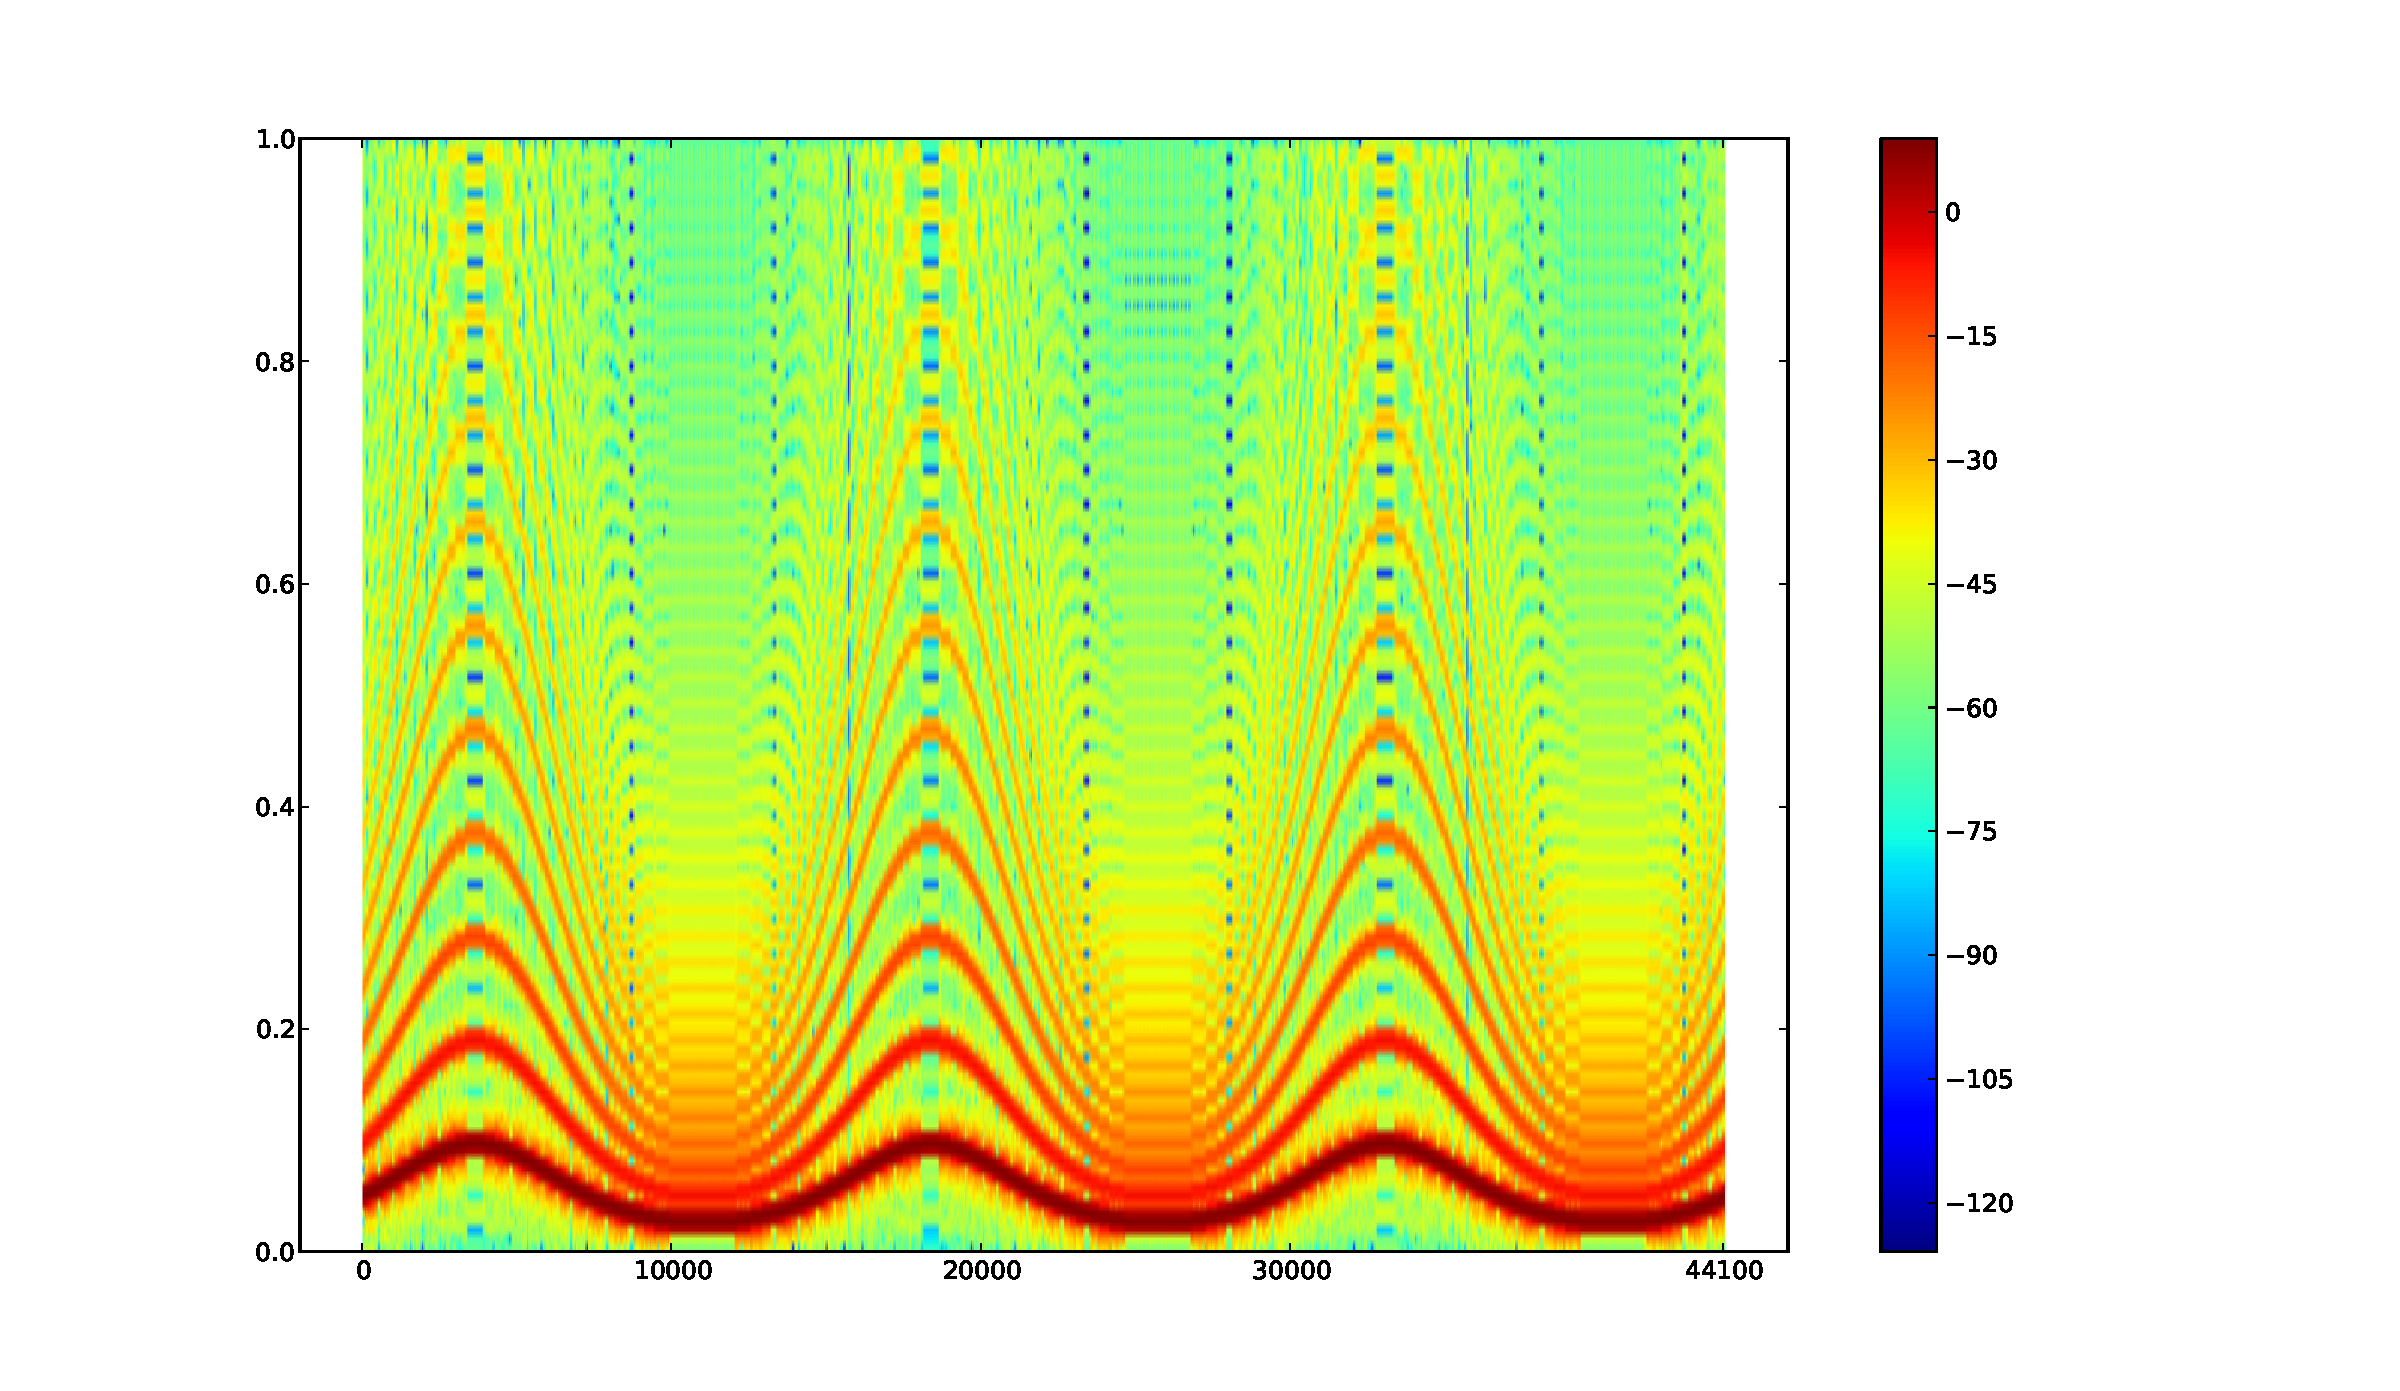
\includegraphics[width=\columnwidth]{figures/vibrato}
     \caption{Spectrogram of a sound with a sinusoidal vibrato of $3Hz$ and one octave of depth in a $1000Hz$ sawtooth wave,  considered $f_s=44.1kHz$.}
         \label{fig:vibrato}
\end{figure}

For the proper realization of the vibrato, it is important to pay attention to both tables and sequences.
Table $\widetilde{M}_i$ with length $\widetilde{\Lambda}_M$ and the sequence with indices $\gamma_i'$ make the sequence $t_i'$ which is the oscillation pattern in the frequency while table $\widetilde{L}_i$ with length $\widetilde{\Lambda}$ and the sequence with indices $\gamma_i$ make $t_i$ which is the sound itself.
Variables $\mu$ and $\nu$ quantify the vibrato intensity: $\mu$ is a direct measure of how many Hertz are involved in the upper limit of the oscillation while $\nu$ is the direct measure of how many semitones (or half steps) are involved in the oscillation ($2\nu$ is the number of semitones between the upper and lower peaks of frequency oscillations of the sound $\{t_i\}$ caused by the vibrato).
It is convenient to use $\nu=\log_{2}\frac{f+\mu}{f} $ in this case because the maximum frequency increase is not equivalent to the maximum frequency diminish, but the semitone variation remains.

Figure~\ref{fig:vibrato} is the spectrogram of an artificial vibrato for a note with $1000Hz$ (between a \emph{B} and a \emph{C}), in which pitch deviation reaches one octave above and one below. Practically any waveform can be used to generate a sound and the vibrato oscillation pattern, with virtually any oscillation frequency and pitch deviation\footnote{The pitch deviation is called 'vibrato depth' and is generally given as semitones or cents, as convenient}.
Those oscillations with precise waveforms and arbitrary amplitudes are not possible in traditional music instruments and, in this way, it introduces novelty in the artistic possibilities.

Tremolo is similar: $f'$, $\gamma_i'$ and $t_i'$ remains the same.
The amplitude sequence to be multiplied by the original sequence $t_i$ turns in:

\begin{equation}\label{trA}
 a_i=10^{\frac{V_{dB}}{20}t_i' } = a_{\text{max}}^{t_i'}
\end{equation}
and finally: 
\begin{multline}\label{trT}
 T_i^{tr(f')}=\left \{ t_i^{tr(f')} \right \}_0^{\Lambda-1}=\{ t_i . a_i \}_0^{\Lambda-1}= \\ =\left \{t_i .10^{t_i' \frac{V_{dB}}{20}}    \right \}_0^{\Lambda-1}=\left\{t_i . a_{\text{max}}^{t_i'} \right\}_0^{\Lambda-1}
\end{multline}

\noindent where $V_{dB}$ is the oscillation depth in decibels of tremolo and $a_{\text{max}}=10^{\frac{V_{dB}}{20}}$ is the maximum amplitude gain.
The measurement in decibels is pertinent because the maximum increase in amplitude is not equivalent to the related maximum decrease, while the difference in decibels remains.

Figure~\ref{fig:tremolo} shows the amplitude of sequences $\{a_i\}_0^{\Lambda-1}$ and $\{t_i'\}_0^{\Lambda-1}$ for three oscillations of a tremolo with a sawtooth waveform. The curvature is due to the logarithmic progression of the intensity. The tremolo frequency is $1,5Hz$ because $f_a=44,1kHz \; \Rightarrow \; \text{duration} = \frac{i_{\text{max}}=82000}{f_a}= 2s \; \Rightarrow \; \frac{3\text{oscillations}}{2s}=1,5$ oscillations per second ($Hz$). 

The music piece \emph{Vibra e treme} explores these possibilities given by tremolos and vibratos, both used in conjunction and independently, with frequencies $f'$, different depths ($\nu$ and $V_{dB}$), and progressive parameters variations (tremolos and vibratos occur many times together in a traditional music instrument and voices). Aiming a qualitative appreciation, the piece also develops a comparison between vibratos and tremolos in logarithmic and linear scales. Its source code is available online as part of the \massa\ toolbox.

\begin{figure*}
     \centering
         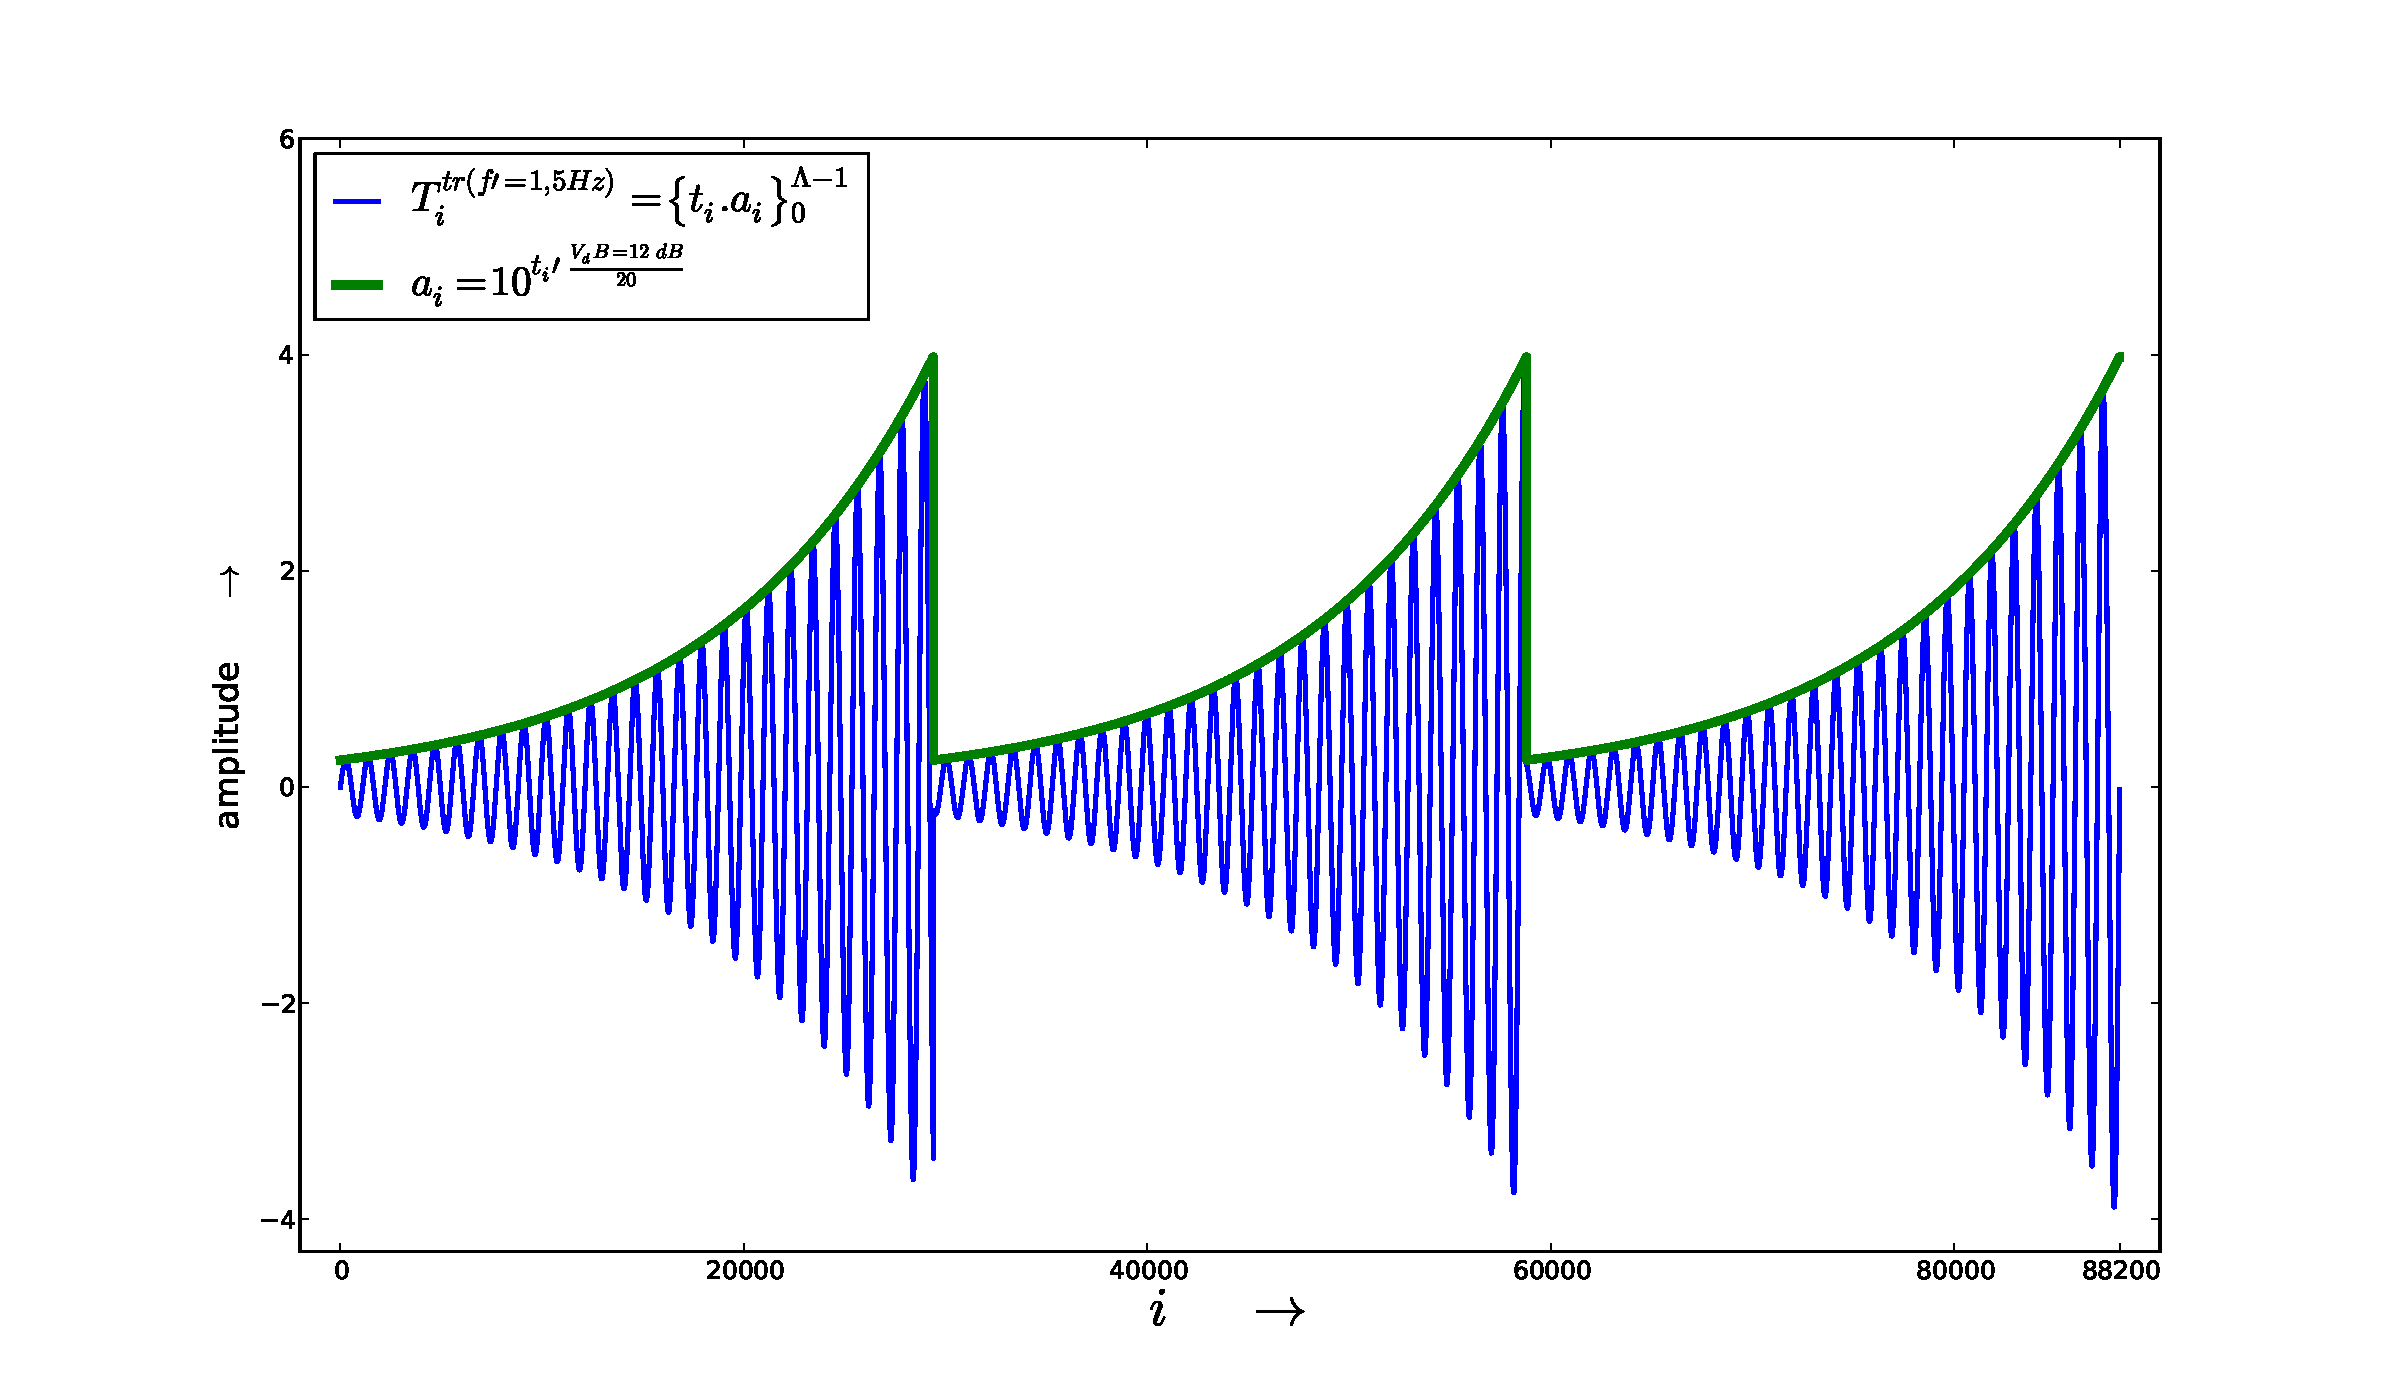
\includegraphics[width=\textwidth]{figures/tremolo}
     \caption{Tremolo with a depth of $V_{dB}=12dB$, with a sawtooth waveform as its oscillatory pattern, with $f'=1.5Hz$ in a sine of $f=40Hz$ (considered a sample frequency of $f_s=44.1kHz$).}
         \label{fig:tremolo}
\end{figure*}

The proximity of $f'$ to $20Hz$ generates rugosity in both tremolos and vibratos. This rugosity is largely appreciated both in
traditional classical music and current electronic music, specially in the \emph{Dubstep} genre.  Rugosity is also generated by spectral content that produce beating~\cite{Porres,porres2009}. The sequence \emph{Bela Rugosi} explores this rugosity threshold with concomitant tremolos and vibratos at the same
voice, with different intensity and waveforms. The respective code is
available online in the \massa\ toolbox.

As frequency increases further, these oscillations no longer remains
noticeable individually. In this case, the oscillations are audible as pitch. Then, $f'$,
$\mu$ and the waveform together, changes the spectrum of original sound $T_i$
in different ways for both tremolos and vibratos.  They are called AM
(\emph{Amplitude Modulation}) and FM (\emph{Frequency Modulation}) synthesis,
respectively.  These techniques are well known, with applications in
synthesizers like \emph{Yamaha DX7}, and even with applications outside music, like
in telecommunications, for data transfer by means of electromagnetic waves (e.g.\ AM and FM radios).

For musical goals, it is possible to understand FM based on the
case of sines and, in occurrences of greater complexity, to decompose the signals into their respective Fourier components (i.e.\ sines as well). In this way, the FM
synthesis performed with a sinusoidal vibrato with frequency $f'$ and depth
$\mu$ in a sinusoidal sound $T_i$ with frequency $f$ generates bands
centered in $f$ and far from each other with a distance of $f'$:

\begin{equation}\label{eq:fmEsp}
\begin{split}
\{t_i'\} & = \left \{ \cos \left [f . 2 \pi \frac{i}{f_s-1} + \mu . sen \left ( f' . 2 \pi \frac{i}{ f_s -1 } \right ) \right ] \right \} = \\
 & = \left \{ \sum_{k=-\infty}^{+\infty} J_k(\mu) \cos \left [ f . 2 \pi \frac{i}{f_s-1} + k . f' . 2 \pi \frac{i}{f_s-1} \right ]  \right \} = \\
 & = \left \{ \sum_{k=-\infty}^{+\infty} J_k(\mu) \cos \left [ (f+k.f') . 2 \pi \frac{i}{f_s-1} \right ]  \right \}
\end{split}
\end{equation}

\noindent where

\begin{multline}\label{eq:Bessel}
J_k(\mu) = \\ = \frac{2}{\pi} \int_0^{\frac{\pi}{2}}\left [ cos \left (\overline{k}\;\frac{\pi}{2} + \mu . \sin w \right ) . cos \left ( \overline{k}\;\frac{\pi}{2} + k . w \right ) \right ] dw \\  \overline{k} = k \% 2 \;\;,\;\; k \in \mathbb{N}
\end{multline}

\noindent is the Bessel function~\cite{BesselCCRMA,JOSFM} which specifies the
amplitude of each component in FM synthesis.

On these equations, the frequency variation introduced by $\{t_i'\}$ does not
respect the geometric progression that yield linear pitch variation, but reflects
equation~\ref{freqLinear}. The use of equations~\ref{vbrF} for FM are described in~\cite{dissertacao}, where the spectral content of the FM synthesis is calculated for oscillations in the logarithmic scale. In
fact, the simple and attractive FM behavior are observed only with linear variations, such as in~\ref{eq:fmEsp}).

For the amplitude modulation (AM): 

\newcommand{\OneColEqu}[1]{%
\end{multicols}%
\begin{twocolequfloat}%
\begin{equation}
\{t_i'\}_0^{\Lambda-1} =\{(1+a_i) . t_i\}_0^{\Lambda-1} = \left \{ \left [ 1+M.\sin \left ( f'.2\pi\frac{i}{f_s -1} \right ) \right] .P .\sin \left ( f.2\pi\frac{i}{f_s -1} \right ) \right \}_0^{\Lambda-1} = \\ 
                        =  \left\{P.\sin \left( f.2\pi\frac{i}{f_s -1}  \right ) +  \frac{P.M}{2} \left [ \sin \left( (f-f').2\pi\frac{i}{f_s -1}  \right )  + \sin \left( (f+f').2\pi\frac{i}{f_s -1}  \right ) \right ] \right \}_0^{\Lambda-1}
\end{equation}
\end{twocolequfloat}%
\begin{multicols}{2}%
}


%\begin{widetext}
%\begin{multline*}\label{eq:amEsp}
%\begin{split}
%\{t_i'\}_0^{\Lambda-1} =\{(1+a_i) . t_i\}_0^{\Lambda-1} = \left \{ \left [ 1+M.\sin \left ( f'.2\pi\frac{i}{f_a -1} \right ) \right] .P .\sin \left ( f.2\pi\frac{i}{f_a -1} \right ) \right \}_0^{\Lambda-1} = \\ 
%                        =  \left\{P.\sin \left( f.2\pi\frac{i}{f_a -1}  \right %) +  \frac{P.M}{2} \left [ \sin \left( (f-f').2\pi\frac{i}{f_a -1}  \right )  + \sin \left( (f+f').2\pi\frac{i}{f_a -1}  \right ) \right ] \right \}_0^{\Lambda-1}
%\end{split}
%\end{multline*}
%\end{widetext}

The resulting sound is the original one together with the
reproduction of its spectral content below and above the original frequency,
with the distance $f'$ from $f$. Again, this is obtained by variations in the
linear scale of the amplitude. An exposition of the
spectrum of an AM performed with oscillations in the logarithmic amplitude scale is again in~\cite{dissertacao}, and it again loses the simple and attractive behavior.

The sequence $T_i$, with frequency $f$, called `carrier', is modulated by
$f'$, called 'modulator'. In FM and AM jargon, $\mu$ and
$\alpha=10^{\frac{V_{dB}}{20}}$ are `modulation indexes'. The following
equations are defined for the vibration pattern of the modulator sequence
$\{t_i'\}$:

\begin{equation}\label{fmGammaAux}
\gamma_i'=\left \lfloor i f' \frac{\widetilde{\Lambda}_M}{f_s} \right \rfloor
\end{equation}

\begin{equation}\label{fmAux}
t_i'=\widetilde{m}_{\gamma_i' \;\% \widetilde{\Lambda}_M}
\end{equation}

The modulator $\{t_i'\}$ into the carrier $\{t_i\}$, for FM, is applied as:

\begin{equation}\label{fmF}
f_i=f + \mu . t_i'
\end{equation}

\begin{equation}\label{fmGamma}
\Delta_{\gamma_i}=f_i\frac{\widetilde{\Lambda}}{f_s} \quad \Rightarrow \quad \gamma_i = \left \lfloor \sum_{j=0}^{i} f_j \frac{\widetilde{\Lambda}}{f_s} \right \rfloor = \left \lfloor \sum_{j=0}^{i} \frac{\widetilde{\Lambda}}{f_s}(f+\mu . t_j') \right\rfloor
\end{equation}

\begin{equation}\label{fmT}
T_i^{f,\, FM(f',\,\mu)}=\left\{ t_i^{f,\,FM(f',\,\mu)} \right\}_0^{\Lambda-1}=\left\{\,\widetilde{l}_{\gamma_i \%\; \widetilde{\Lambda} } \,\right\}_0^{\Lambda-1}
\end{equation}


\noindent where $\widetilde{l}$ is the waveform period with a length of
$\widetilde{\Lambda}$ samples, used for the carrier signal.

To perform AM, it is needed to modulate the signal $\{t_i\}$ with $\{t_i'\}$ using
the following equations:

\begin{equation}\label{amA}
a_i=1 + \alpha . t_i'
\end{equation}

\begin{multline}\label{amT}
T_i^{f,\,AM(f',\,\alpha)}=\left\{ t_i^{f,\,AM(f',\,\alpha)} \right\}_0^{\Lambda-1}=\{ t_i . a_i \}_0^{\Lambda-1}= \\ \{t_i . (1 + \alpha . t_i')    \}_0^{\Lambda-1}
\end{multline}


\subsection{Musical usages}\label{subsec:mus2}

At this point, the musical possibilities exploded. All characteristics, like pitch (given by frequency), timbre (given by the waveform, filters and noise), volume (manipulated by intensity) and duration (given by the number of samples), can be considered in an absolute form or treated during duration of sound (clearly, with the exception of duration itself).

The following musical usages comprehend a collection of possibilities
with the purpose of exemplifying types of sound manipulation that result in
musical material. Some of them are deeply discussed in the next section.


\subsubsection{Relations between characteristics}

An interesting possibility is to use relations between parameters of
a tremolo or vibrato, and some parameters of the basic note like frequency. In
this way, it is possible to have a vibrato frequency proportional
to note pitch, or a tremolo depth inversely proportional to
pitch. Therefore, with equations \ref{vbrGamma}, \ref{vbrF} and \ref{trA}, it is
perfectly possible to arbitrate:

\begin{equation}\label{eq:vinculos}
\begin{split}
f^{vbr} = f^{tr} & = func_a(f) \\
\nu & = func_b(f) \\
V_{dB} & = func_c(f)
\end{split}
\end{equation}

\noindent with $f^{vbr}$ and $f^{tr}$ as $f'$ in the referenced equations. They can also be associated with vibrato and tremolo oscillation frequency of
equation~\ref{vbrGamma}. 
 $\nu$ and $V_{dB}$ are the respective depth values of vibrato and
tremolo. Functions $func_a$, $func_b$ and $func_c$ are arbitrary and dependent
on musical intentions. The music piece \emph{Tremolos, vibratos e a
frequência} explores such bonds and exhibit variations in the oscillation
waveform with the purpose of building a \emph{musical
language} (details in the next section). The corresponding code is on
is also available online as part of the \massa\ toolbox.

\subsubsection{Convolution for rhythm and meter}
It is possible to use a musical pulse -- such as specified by a BPM
tempo -- and to place an impulse at the start of each beat, with the purpose of
establishing metric and rhythms: the
convolution with an impulse shifts the sound 
to impulse position.
For example, two impulses equally spaced builds a binary division into the
pulse. Two signals, one with 2 impulses and the other with 3 impulses, both 
equally spaced in the pulse duration, yields a pulse
maintenance with a rhythmic in which eases both binary or ternary
divisions of the pulse, and this is found in many ethnic and traditional musical styles~\cite{Gramani}. 
Absolute values of the impulses implyes in proportions among the
amplitudes of the sonic reincidences.
The use of convolution with impulses in this context is explored in the
music piece \emph{Trenzinho de caipiras impulsivos}. These features
embrace the creation of `sound amalgams' based on granular synthesis, for now refer specially to the
figure~\ref{fig:pulsoSubAgl}. This piece is a link to next section contents. 
The source code of the music piece is online, as part of the \massa toolbox.


\subsubsection{Moving source and receptor, Doppler effect}

Retaken the exposition in subsection~\ref{subsec:spac}, when an audio source
or receptor is moving, its characteristics are ideally updated at each
sample of the digital signal. Speed components should be found for each ear.
In this way, given the audio source speed (or velocity) $v_s$,
with positive values if the source moves away from receptor, and receptor speed $v_r$,
positive when it gets closer to audio source, the frequency is given
by the well known Doppler shift:

\begin{equation}\label{eq:fDoppler}
    f=\left(\frac{v_{sound}+v_r}{v_{sound}+v_s}\right)f_0
\end{equation}

With both frequencies $f$ and $f_0$, and the IID from the new source
position, it is possible to create the Doppler effect. There is an addendum to
improve the fidelity of the physical phenomena: to increase the received
potency. It is possible to understand this potency gain as being proportional 
to the wave shrinking or expansion: $\Delta P=P_0\left(\frac{v_r-v_s}{343.2}\right)$,
 where $P_0$ is signal potency and $P$ the potency at receptor.

In this way, it is possible to obtain both amplitude and frequency of a moving
audio source. Being this audio source in front of receptor with $y_0$ meters of horizontal distance and $z_0$ meters of height, the distance is given by
$D_i=\left\{ d_i=\sqrt{ y_{i}^{2}+z_{0}^{2} } \right\}_0^{\Lambda-1}$,
where $y_i=y_0+(v_s-v_r)\frac{i}{f_s}$ with $v_s$ and $v_r$ both
horizontal, having null non-$y$ components. Amplitude changes with the distance and with the potency factor cited
above (see subsection~\ref{subsec:volume} for potency to amplitude conversion).

\begin{equation}\label{eq:aDoppler}
    A_i=\left\{ \frac{z_0}{d_i}A_{\Delta P}\right\}_0^{\Lambda-1} = \left\{ \frac{z_0}{\sqrt{y_i^2+z_0^2}} \sqrt{\frac{v_r-v_s}{343,2}+1}  \,\right\}_0^{\Lambda-1}
\end{equation}

The amplitude change caused by the distance is even, while the change caused by the potency variation is antisymmetric in
relation to the crossing of source with receptor. The frequency has a symmetric progression in relation to pitch. In other words, the same semitones (or fractions) added during the approach are decreased during the departure. Besides that, the transition is abrupt if source and receptor intersect with zero distance, otherwise, there is a monotonic progression. In the given case, where there is a static height $z_0$, observed the speed component in the direction given by observer and source positions, the frequencies $F_i$ at the observer is given by:

\begin{equation}\label{eq:ffDoppler}
    F_i=\{f_i\}_0^{\Lambda-1}=\left\{\frac{v_{sound} + v_r\frac{y_i}{\sqrt{z_0^2+y_i^2}}}{v_{sound}+v_s\frac{y_i}{\sqrt{z_0^2+y_i^2}}}f_0\right\}_0^{\Lambda-1}
\end{equation}

There is a Python implementation of the Doppler
effect as describe above, and also considering the intersection between audio source and receptor,
at the \massa\ toolbox~\cite{massa}.


\subsubsection{Filters and noises (subsections~\ref{subsec:ruidos} and~\ref{subsec:filtros})}

With the use of filters, the possibilities are even wider.
Convolve a signal to have a reverberated version of it, to remove its noise, to
distort or to treat the audio aesthetically in other ways. For
example, it is possible to simulate sounds as if originated in an old television or telefone,
by the use of a band-pass filter, allowing only frequencies between $1kHz$ and $3kHz$.
By rejecting the frequency of electric oscillation (usually $50Hz$ or $60Hz$) and harmonics, one can remove noises
caused by audio devices connected to a usual power suply. A more musical application is to perform filtering in
specific bands and to use those bands as an additional parameter to the notes.

Inspired by traditional music instruments, it is possible to apply a
time-dependent filter~\cite{Roederer}. Chains of these filters can perform
complex and more accurate filtering routines. The music piece \emph{Ruidosa
faixa} explores filters and many kinds and noise
synthesis. The source code is available
online as part of \massa\ toolbox.

A sound can be altered through different filtering and then mixed to create an effect known
as \emph{chorus}. Based on what happens in a choir of singers,
the sound is performed using small and potentially arbitrary
modifications of parameters like center frequency, presence (or absence) of
vibrato or tremolo and its characteristics, equalization, volume, etc. As a
final result, those versions of the original sound are mixed together (see
equation~\ref{eq:mixagem}). The music piece \emph{Chorus infantil} implements a
chorus in many ways with different sounds and its source code is also available in the \massa\ toolbox.


\subsubsection{Reverberation}\label{subsubsec:reverb}

Using the same terms of subsection~\ref{subsec:spac}, the
late reverberation can be achieved by a convolution with a section of pink, brown
or black noise, with exponential decay of amplitude along time.
Delay lines can be added as a prefix to the noise
with the decay, and this contemplates both time parts of the reverberation: the
first reflections and the late reverberation. It is possible to improve the
quality by calculating the geometric trajectory and (mainly low-pass, subsection~\ref{subsec:filtros}) filtering by each surface where
wavefront reflected before reaching the ear in the first $100-200$ milliseconds.
The colored noise can be gradually introduced with a \emph{fade-in}: the initial moment given by direct
incidence of sound (i.e.\ without any reflection and given by ITD and IID),
reaching its maximum at the beginning of the 'late
reverberation', when the geometric incidences loses their relevance to the
statistical properties of noise decay.

As an example, consider $\Delta_1$ as the duration of the first section and $\Delta_R$ as the duration of total reverberation ($\Lambda_1=\Delta_1 f_s$, $\Lambda_R=\Delta_R
f_s$). Be $p_i$ the probability of a sound to repeat in the
$i$-th sample. Amplitude falls with exponential decay. Following
subsection~\ref{subsec:spac}, the reverberation $R_i^1$ of the first period can
be described as:

\begin{equation}\label{eq:p1rev}
\begin{split}
    R_i^1=\left\{r_i^1\right\}_0^{\Lambda_1-1}\;:\quad\quad\quad\quad\quad\quad\quad\quad \\ 
\;r_i^1=\left\{
        \begin{array}{l l}
            10^{\frac{V_{dB}}{20}\frac{i}{\Lambda_R-1}}\;  & \text{with probability}\quad p_i=\left(\frac{i}{\Lambda_1}\right)^2 \\
                                     0 \; & \text{with probability}\quad 1-p_i \\
        \end{array} \right.
\end{split}
\end{equation}

\noindent where $V_{dB}$ is the total decay in decibels, typically $-80dB$ or
        $-120dB$. Reverberation $R_i^2$ of the second period can be emulated by a
        brown noise $R_i^m$ (or by a pink noise $R_i^r$) with exponential amplitude decay of the waveform:

\begin{equation}\label{eq:p2rev}
    R_i^2=\left\{r_i^2\right\}_{\Lambda_1}^{\Lambda_R-1}=\left\{10^{\frac{V_{dB}}{20}\frac{i}{\Lambda_R-1}}\,.\,r_i^m\right\}_{\Lambda_1}^{\Lambda_R-1}
\end{equation}

Considered:

\begin{equation}\label{eq:rev}
    R_i=\left\{r_i\right\}_0^{\Lambda_R-1}\;:\;r_i=\left\{
        \begin{array}{l l}
            1\; & \text{if }\quad i=0 \\
            r_i^1\;  & \text{if }\quad 1\leq i<\Lambda_1-1 \\
                                     r_i^2 \; & \text{se}\quad \Lambda_1 \leq i < \Lambda_R-1 \\
        \end{array} \right.
\end{equation}

\noindent, a reverberated auralization of a sound can be achieved by simple
        convolution of $R_i$ (called reverberation 'impulse response') with the sound sequence $T_i$ as described in subsection~\ref{subsec:filtros}.

Reverberation is well known by causing great interest in the listeners and to provide more enjoyable sonorities. Besides that, modifications in the reverberation space consists on a common resource (almost a \textit{clich\'{e}}) to surprise and attract the listener. An implementation of the reverb recipe described is on the \massa\ toolbox~\cite{massa}


\subsubsection{ADSR Envelopes}

The volume variation along the duration of sound is crucial to our timbre
perception. The volume envelope known as ADSR (\emph{Attack-Decay-Sustain-Release}), 
has many implementations in both hardware and software synthesizers. 
A pioneer implementation can be found in the Hammond
Novachord synthesizer of 1938 and some variants are cited below~\cite{ADSR}.

The scholastic ADSR envelope is characterized by 4 parameters: attack duration
(time in which sound reaches its maximum amplitude), decay duration (follows the attack
immediately), level of sustain volume (in which the volume remains stable after the decay) and release duration (after sustain section, this is the duration needed for amplitude to reach zero or final value).
Note that the sustain duration is not specified because it is the difference between the duration itself and the durations of attack, decay and sustain.

The ADSR envelope with durations $\Delta_A$, $\Delta_D$ and $\Delta_R$, with total duration $\Delta$ and sustain level $a_S$, given by the fraction of the maximum amplitude, to be aplyed to any sound sequence $T_i=\{t_i\}$, can be presented as:

\begin{equation}\label{eq:adsr}
\begin{split}
\{a_i\}_0^{\Lambda_A-1}  = & \left\{\xi\left(\frac{1}{\xi}\right)^{\frac{i}{\Lambda_A-1}}\right\}_0^{\Lambda_A-1} \quad \text{ or }\\ = & \left\{\frac{i}{\Lambda_A-1}\right\}_0^{\Lambda_A}\\
\{a_i\}_{\Lambda_A}^{\Lambda_A+\Lambda_D-1} = & \left\{a_S^{\frac{i-\Lambda_A}{\Lambda_D-1}}  \right\}_{\Lambda_A}^{\Lambda_A+\Lambda_D-1} \quad \text{ or } \\ = &  \left\{1-(1-a_S)\frac{i-\Lambda_A}{\Lambda_D-1}\right\}_{\Lambda_A}^{\Lambda_A+\Lambda_D-1}\\
\{ a_i \}_{\Lambda_A+\Lambda_D}^{\Lambda-\Lambda_R-1} = & \left\{ a_S \right\}_{\Lambda_A+\Lambda_D}^{\Lambda-\Lambda_R-1} \\
\{ a_i \}_{\Lambda-\Lambda_R}^{\Lambda-1}  = & \left\{ a_S\left(\frac{\xi}{a_S} \right)^{\frac{i-(\Lambda-\Lambda_R)}{\Lambda_R-1}} \right\}_{\Lambda-\Lambda_R}^{\Lambda-1} \quad \text{ or } \\ = &  \left\{ a_S - a_S\frac{i+\Lambda_R-\Lambda}{\Lambda_R-1}\right\}_{\Lambda-\Lambda_R}^{\Lambda-1} 
\end{split}
\end{equation}


\noindent with $\Lambda_X=\lfloor \Delta . f_s \rfloor\;\;\forall\;\; X \; \in
(A,D,R,\;)$ and being $\xi$ a small value that provides a satisfactory \emph{fade in} and \emph{fade out}, e.g.\ $\xi=10^{\frac{-80}{20}}=10^{-4}\;$ or $\;\xi=10^{\frac{-40}{20}}=10^{-2}$. The lower the $\xi$, the slower the \emph{fade}, like the $\alpha$ illustrated in Figure~\ref{fig:transicao}. The stated second in equations~\ref{eq:adsr} attend both introduction and ending of sound from zero intensity because they are linear. Schematically, figure~\ref{fig:adsr} shows the ADSR envelope in a classical implementation that supports many variations. For example, between attack and decay it is possible to add an extra partition where the maximum amplitude remains for more than a peak. Another common example is the use of more elaborated tracings of attack or decay. The music piece \emph{ADa e SaRa}, available 
in \massa, explores many configurations of the ADSL envelope.

\begin{equation}\label{eq:adsrApl}
\left\{t_i^{ADSR}\right\}_0^{\Lambda-1} =\{t_i . a_i\}_0^{\Lambda-1}
\end{equation}

\begin{figure}[htpq!]
    \centering
        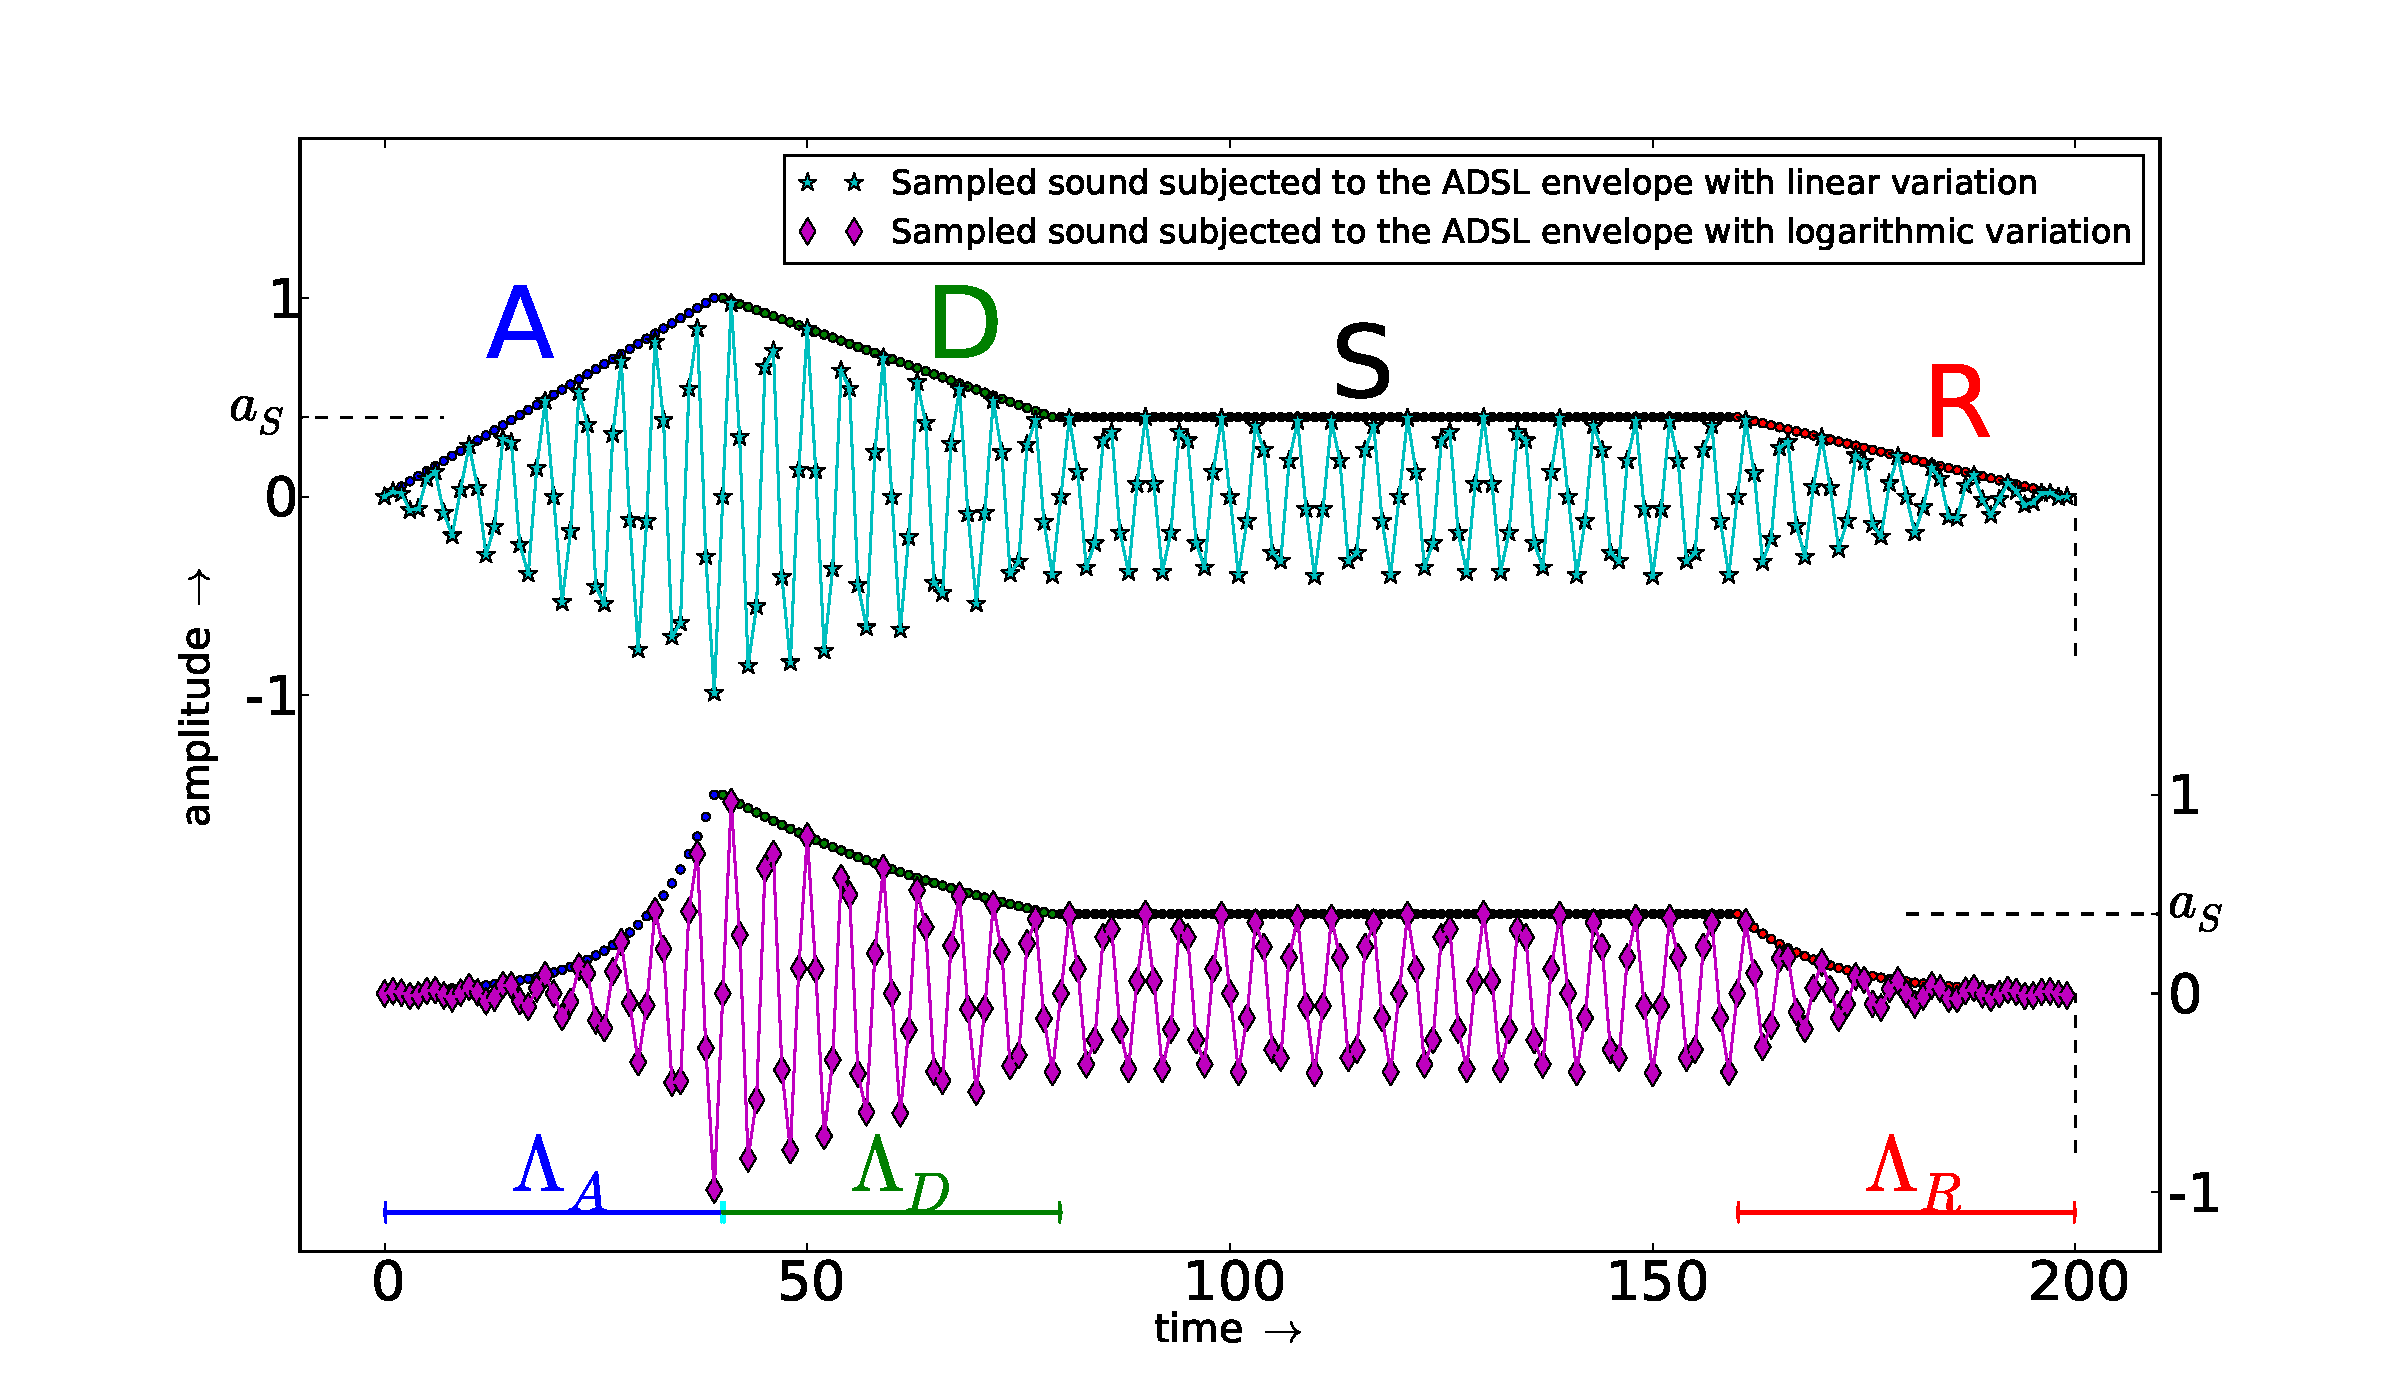
\includegraphics[width=\columnwidth]{figures/adsr}
    \caption{An ADSR envelope (\emph{Attack, Decay, Sustain, Release}) applied
        to an arbitrary sound sequence. The linear variation of the amplitude is
        above, in blue. Below the amplitude variation is exponential.}
        \label{fig:adsr}
\end{figure}

%%%%%%%%%%%%%%%%%%%%%%%%%%%%%%%%%%%%%%%%%%%%%%%%%%%%%%%%%%%%%%%%%%%%%%%%%%%%%%%
%%%%%%%%%%%%%%%%%%%%%%%%%%%%%%%%%%%%%%%%%%%%%%%%%%%%%%%%%%%%%%%%%%%%%%%%%%%%%%%
%%%%%%%%%%%%%%%%%%%%%%%%%%%%%%%%%%%%%%%%%%%%%%%%%%%%%%%%%%%%%%%%%%%%%%%%%%%%%%%
%%%%%%%%%%%%%%%%%%%%%%%%%%%%%%%%%%%%%%%%%%%%%%%%%%%%%%%%%%%%%%%%%%%%%%%%%%%%%%%
%%%%%%%%%%%%%%%%%%%%%%%%%%%%%%%%%%%%%%%%%%%%%%%%%%%%%%%%%%%%%%%%%%%%%%%%%%%%%%%
%%%%%%%%%%%%%%%%%%%%%%%%%%%%%%%%%%%%%%%%%%%%%%%%%%%%%%%%%%%%%%%%%%%%%%%%%%%%%%%

%\afterpage{\blankpage}

%\clearpage


\section{Organization of notes in music}\label{notasMusica} \label{sec:notesMusic}

Consider $ S_j=\left\{  s_j=T_i^j=\{t_i^j\}_{i=0}^{\Lambda_j-1} \right\}_{j=0}^{H-1} $, the sequence $S_j$ of $H$ musical events $s_j$. Be $S_j$ a `musical structure', composed by events $s_j$ which are musical structures themselves, e.g.\ notes. This section is dedicated to techniques that make $S_j$ interesting and enjoyable for audition.

The elements of $S_j$ can be overlapped by mixing them together, as in
equation~\ref{eq:mixagem} and figure~\ref{fig:mixagem}, for building intervals
and chords. This reflects the `vertical thought' in music. On the other hand, the concatenation of the events
in $S_j$, as in equation~\ref{eq:concatenacao} and in figure ~\ref{fig:concatenacao},
builds melodic sequences and rhythms, which are associated with the musical
`horizontal thought'. The fundamental frequency $f$ and the starting moment
(attack) are generally the most important characteristics of the elements $s_j$ in
$S_j$. This makes possible the creation of music made by pitches (both
harmony and melody) and by the presence of temporal metrics and rhythms.

\subsection{Tuning, intervals, scales and chords}\label{subsec:afinacao}

\subsubsection{Tuning}

Doubling the frequency is equivalent to ascending one octave ($f=2f_0$).
The octave division in twelve steps is the canon of classical western music.
Its usage has also been observed
outside western tradition, like ceremonial/religious and ethnic context~\cite{Wisnick}.
In this system, ideally, the factor given by $\varepsilon=2^{\frac{1}{12}}$ defines a semitone.
A note grid along the hearing spectrum in which, given the frequency $f$, all the possible
fundamental frequencies are separated by intervals, multiples of
$\varepsilon$. Twelve semitones (or half steps), equidistant to the human ear, reaches an
octave, equivalent to human year. Therefore, if $f=2^{\frac{1}{12}}f_0$, there is a semitone between
$f_0$ and $f$.

This absolute accuracy is common in computational implementations. Real
music instruments, however, exhibit deviations in order to make compatible
deviations from the harmonics of notes. Besides that, the fixed reference
$\varepsilon=2^{\frac{1}{12}}$ characterizes an equally tempered tuning. There
are tunings in which intervals are ratios of low-order integers, based
on observations of physical phenomena. These tunings were first formalized
around two thousand years before the arrival of the equal temperament~\cite{Roederer}.
). Two emblematic tunings are:

\begin{itemize}
    \item The {\bf just intonation}, defined by association of diatonic scale notes
    with ratios of low-order integers, as found in the harmonic
    series. Considered the ionian mode, the white piano keys
    from C to C, as seen below in subsection~\ref{subsec:escalas}, i.e. intervals 1, 2M, 3M, 4J, 5J, 6M, 7M, 8,
    are considered ratios of frequency: 1, 9/8, 5/4
    4/3, 3/2, 5/3, 15/8, 2/1. 
    The following intervals are also considered: the
    semitone 16/15, the 'minor tone' 10/9, and the 'major tone' 9/8.
    There are many ways to perform the division of the 12 notes in the just intonation.

    \item The {\bf Pythagorean tuning}, based on the interval 3/2 (perfect
    fifth). The Ionian mode ratios becomes: 1, 9/8, 81/64, 4/3, 3/2, 27/16, 243/128,
    2/1. These intervals are also considered to yield notes in a scale. Besides the
    intervals in the mode, also used are the minor second 256/243, the minor
    third 32/27, the augmented fourth 729/512, the diminished fifth 1024/729,
    the minor sixth 128/81 and the minor seventh 16/9. 
\end{itemize}

In order to attend for micro-tonality\footnote{Micro-tonality is the use of intervals less
than one semitone and have ornamental and structuring functionalities in music. The
division of the octave in $12$ notes is motivated by physical fundaments but also
a \emph{convention} adopted too by western classical music. Other tunings are
incident. To point only one example, the traditional Thai music uses an octave
division in seven notes equally spaced ($\varepsilon=2^{\frac{1}{7}}$),
which allows intervals that have little in common with the intervals in the
diatonic scale~\cite{Wisnick}}. It is possible to use non-integer real values as
factors of $\varepsilon=2^{\frac{1}{12}}$ between frequencies, 
or to maintain integer values and change $\varepsilon$. For example, 
a tuning really near of the harmonic series
itself is proposed with the equal division of the octave in $53$ notes:
$\varepsilon_2=2^{\frac{1}{53}}$.~\cite{microtonalidade}
In this division, notes are related by means of integers, factors of
$\varepsilon_2$ relating frequencies by a valid interval.
 Note that if $S_i$ is a pitch sequence related by means of
$\varepsilon_1$, a direct mapping for notes related by $\varepsilon_2$ is 
a new sequence $S_i'=\left\{s_i'\right\}=\left\{
s_i \frac{\varepsilon_1}{\varepsilon_2}\right\}$. The music piece \emph{Micro
tom} explores microtonal features and its code
is part of \massa\ toolbox.


\subsubsection{Intervals}\label{subsec:intervalos}

Using the ratio $\varepsilon=2^{\frac{1}{12}}$ between note frequencies
(i.e.\ one semitone) the intervals in the twelve note system can be represented by integers.
Table~\ref{eq:intervalos} summarizes each interval:
 its traditional nomenclature, consonance and
dissonance properties, and number of semitones.

\begin{table*}[htpq!]
\centering
\caption{Music intervals together with their traditional notation, basic classification for dissonance and consonance, and number of semitones. Unison, fifth and octave are the perfect (P) consonances. Major (M) and minor (m) thirds and sixths are the imperfect consonances. Minor seconds and major sevenths are the harsh dissonances. Major seconds and minor sevenths are the mild dissonances. Perfect fourth is a special case, being a perfect consonance when considered as an inversion of the perfect fifth and a dissonance or a imperfect consonance otherwise. The second special case is the tritone (A4 or aug4, d5 or dim5, tri, TT). This interval is consonant in some cultures.
For tonal music, the tritone indicates dominant and seeks urgent resolution in a third or sixth.
Due to this instability it is considered a dissonant interval.}
\begin{tabular}{| c | c | c | }\hline
    \multicolumn{3}{|c|}{\bf consonances}  \\\hline
   & traditional notation & number of semitones \\
   perfects: & P1, P5, P8 & 0, 7, 12 \\
 imperfects: & m3, M3, m6, M6 & 3, 4, 8, 9 \\\hline\hline
    \multicolumn{3}{|c|}{\bf dissonances} \\\hline
 & traditional notation & number of semitones \\
 fortes: & m2, M7 & 1, 11 \\
 brandas: & M2, m7 & 2, 10 \\\hline\hline
    \multicolumn{3}{|c|}{\bf special cases} \\\hline
 & traditional notation & number of semitones \\
 consonance or dissonance: & P4 & 5 \\
 dissonance in Western tradition: & tritone, aug4, dim5 & 6 \\\hline
\end{tabular}\label{eq:intervalos}
\end{table*}

The nomenclature, based on conveniences for tonal music and practical aspects of note manipulation, can be specified
as follows~\cite{Roederer,Wisnick}:

\begin{itemize}
                \item Intervals are seen first by the as number of steps between notes: first
                (unison), second, third, forth, fifth, sixth, seventh and
                eighth (octave). The ninth, tenth, eleventh, etc, are compound  
                intervals made by one or more octaves plus a ``simple'' interval inside the
                octave, which characterizes the compound interval. The
                intervals are represented by numeric digits, e.g. 1, 3, 5
                are a unison, a third and a fifth, respectively.

                \item Qualities of each interval: perfect consonances --
                i.e.\ unison, forth, fifth and octave -- are 'perfect'. The
                imperfect consonances -- i.e.\ thirds and sixths -- and
                dissonances -- i.e.\ seconds and sevenths -- can be major and
                minor. Exception for the tritone.

                \item The perfect fourth can be a perfect consonance or
                a dissonance according to the context and theoretical
                background. As a general rule, it can be considered
                a consonance except when it resolves into a
                fifth or a third with movimentation of just one note .

                \item Tritone is a dissonance in Western music because
                it characterizes the ``dominant'' chord in the tonal system (see
                subsection~\ref{subsec:harmonia}) and represents the
                instability. Some cultures have the interval as a consonance,
                using it in melodies and chants as a stable interval. 

                \item A major interval decreased by one semitone results in a
                minor interval. A minor interval increased by one semitone
                results in a major interval.

                \item A perfect interval (unison, perfect forth, perfect
                fifth, perfect octave), or a major interval (major second M2,
                major third M3, major sixth M6 or major seventh M7), increased
                by one semitone results in an augmented interval (e.g.\
                augmented third aug3 with five semitones). The augmented forth
                is also called tritone (aug4 ~ tri ~ TT).

                \item A perfect interval or a minor interval (minor second m2,
                minor third m3, minor sixth m6 or minor seventh m7), decreased
                by one semitone results in a diminished interval. The
                diminished fifth is also called tritone (dim5 ~ tri ~ TT).

                \item An augmented interval increased by one semitone results
                 in a `doubly augmented' interval and a diminished interval
                decreased by one semitone results in a `doubly diminished'
                interval.

                \item Notes played simultaneously configure a harmonic
                interval.

                \item Notes played as a sequence in time configure a
                melodic interval. The order of the notes: first
                the lowest note or the highest note, results in an ascending
                 or descending interval, respectively.

                \item If the lower pitch is raised one octave, or if
                the upper pitch is lowered one octave, the interval is
                inverted. The sum of an interval and its inversion is
                9 (e.g.\ m7 is inverted to M2: $m7+M2=9$). An inverted major
                interval results in a minor interval and vice-versa. An
                inverted augmented interval results in a diminished interval
                and vice-versa (inverting a doublyi-augmented results in a
                doubly-diminished and vice-verse, etc.).
                An inverted perfect interval results in a perfect interval as well.

                \item An interval higher than an octave is called a 'compound
                interval' and is classified like the interval between the same
                notes but in the same octave. They are also reached by adding a
                7 to the interval: P11 is an octave plus a forth ($7 + P4 = P11$),
                M9 is an octave plus a major second ($7 + M2 = M9$).
\end{itemize}

The augmented/diminished intervals and the doubly augmented/doubly diminished intervals are consequences of the tonal system.
Scale degrees (subsection~\ref{subsec:escalas}) are in fact different pitches, with
specific uses and functions. Henceforth, in a \textit{C flat} major scale, the tonic -- first degree -- is \textit{C flat}, not \textit{B}, and the leading tone -- seventh degree -- is \textit{B flat}, not \textit{A sharp} or \textit{C double flat}. In a similar way, the second degree of a scale can be one semitone from first degree, like the leading tone (seventh degree at one ascending semitone from the first degree), where there is a diminished third between the two semitones of the seventh and second scale degrees~\cite{Lacerda}.

The descriptions presented summarizes the traditional theory of the music
intervals~\cite{Lacerda}. The music piece \emph{Intervalos entre alturas}
explores these intervals in both independent and related manners. 
The source code is available online in the \massa\ toolbox~\cite{MASSA}.

\subsubsection{Scales}\label{subsec:escalas}

A scale is an ordered set of pitches. Usually, scales repeat at each octave. 
The ascending sequence with all notes from the octave division in 12 equal intervals, 
separated by the ratio $\varepsilon=2^{\frac{1}{12}}$, is known as the chromatic scale with equal temperament.
There are 5 perfectly symmetric divisions of the octave within the chromatic scale. 
These divisions are considered scales by easy and peculiar uses they provide.
Considering integers $e_i$ used as powers of the factor $\varepsilon=2^{\frac{1}{12}}$
to multiply lower note frequency ($f=\varepsilon^{e_i} f_0$),
the scales are as follows:

\begin{equation}\label{escSim}
\begin{split}
\text{chromatic}    & = E_i^c = \{e_i^c\}_0^{11} = \\
                    & =  \{0,1,2,3,4,5,6,7,8,9,10,11\} = \{i\}_0^{11}\\
\text{whole tones}  & = E_i^t = \{e_i^t\}_0^{5} = \{0,2,4,6,8,10\} = \{2.i\}_0^{5} \\
\text{minor thirds} & = E_i^{tm} = \{e_i^{tm}\}_0^{3} = \{0,3,6,9\} = \{3.i\}_0^3 \\
\text{major thirds} & = E_i^{tM} = \{e_i^{tM}\}_0^{2} = \{0,4,8\} = \{4.i\}_0^2\\
\text{tritones}     & = E_i^{tt} = \{e_i^{tt}\}_0^{1} = \{ 0, 6 \} = \{6.i\}_0^1
\end{split}
\end{equation}

Therefore, the third note of the whole tone scale with $f_0=200Hz$
is $f_3=\varepsilon^{e_3^t} . f_0 = 2^{\frac{6}{12}} . 200 \approxeq 282.843
Hz$. These `scales', or patterns, generate stable structures by their intern
symmetries and can be repeated in an efficient and sustained way.
Section~\ref{estCic} specially discusses symmetries. 
The music piece \emph{Cristais} exposes each one of these scales, in both melodic and
harmonic counterpart and their source code is part of \massa\ toolbox.

Diatonic modes are:

\begin{equation}\label{eq:escalas}
\begin{split}
\text{aeolian}    & = \text{natural minor scale} = \\
                  & = E_i^m = \{e_i^m\}_0^6 = \{0,2,3,5,7,8,10\} \\
\text{locrian}    & = E_i^{mlo} = \{e_i^{mlo}\}_0^6 = \{0,1,3,5,6,8,10\} \\ 
\text{ionian}     & = \text{major scale} =  \\
                       & = E_i^M = \{e_i^M\}_0^6 = \{0,2,4,5,7,9,11\} \\
\text{dorian}     & = E_i^{md} = \{e_i^{md}\}_0^6 = \{0,2,3,5,7,9,10\} \\
\text{phrygian}   & = E_i^{mf} = \{e_i^{mf}\}_0^6 = \{0,1,3,5,7,8,10\} \\
\text{lydian}     & = E_i^{ml}=\{e_i^{ml}\}_0^6 = \{0,2,4,6,7,9,11\} \\
\text{mixolydian} & = E_i^{mmi} = \{e_i^{mmi}\}_0^6 = \{0,2,4,5,7,9,10\}
\end{split}
\end{equation}

\noindent They have only major, minor and perfect intervals.
The unique exception is the tritone that is presented as an augmented forth or a diminished fifth.

Diatonic scales follow a circular pattern of successive intervals \textit{tone,
tone, semitone, tone, tone, tone, semitone}. Thus, it is possible to write:

\begin{equation}\label{eq:relacaoDia}
\begin{split}
\{d_i\} & =\{2,2,1,2,2,2,1\} \\
e_0 & =0 \\
e_i & =d_{(i+\kappa)\%7}+e_{i-1} \quad for \;\;  i > 0
\end{split}
\end{equation}

\noindent with $\kappa \in \mathbb{N}$. For each mode there is only one value
for $\kappa \in [0,6]$ by which $\{e_i\}$ matches. 
For example, a brief inspection reveals that
$e_i^{ml}=d_{(i+2)\%7}+e_{i-1}^{ml}$. Then, $\kappa=2$ for the lydian mode.

The minor scales has two additional forms, named melodic and harmonic:

\begin{equation}\label{eq:escalasMenores}
\begin{split}
\text{natural minor}&  = E_i^m = \{e_i^m\}_0^6 = \\
                                           &  = \{0,2,3,5,7,8,10\} \\
\text{harmonic minor}                      &  = E_i^{mh} = \{e_i^{mh}\}_0^6 = \\
                                           &  = \{0,2,3,5,7,8,11\} \\
\text{melodic minor}                       &  = E_i^{mm} = \{e_i^{mm}\}_0^{14} = \\
                                           &  = \{0,2,3,5,7,9,11,12,10,8,7,5,3,2,0\} \\
\end{split}
\end{equation}

The different ascending and descending contour of the melodic minor scale is required
by the leading tone (seventh and last degree, separated by 
one semitone from the octave, enhances tonic polarization) in the ascending
 trajectory, which is not necessary in the descending mode, and therefore it recovers the normal form.
The harmonic scale presents the leading tone but does not avoid the augmented second
between the sixth and seventh degrees, it does not consider the melodic trajectory~\cite{Harmonia}. 
Other scales can be represented in a similar form, like the pentatonic and the
modes of limited transposition by Messiaen~\cite{Messiaen}. 

Although not a scale, the harmonic series is often used as such.
Besides, this point is a convenient moment to put it plain simple:

\begin{equation}\label{eq:serieHarmonica}
\begin{split}
H_i = & \{h_i\}_0^{19}= \\
      & \{ 0,12,19+0.02,  24,28-0.14, 31+0.2, 34-0.31, \\
                     & 36, 38+0.04,40-0.14, 42-0.49, 43+0.02, \\
                     & 44+0.41, 46-0.31, 47-0.12, \\
                     & 48, 49+0.05, 50+0.04, 51-0.02, 52-0.14   \}
\end{split}
\end{equation}

In this scale, the frequency of $i-th$ note $h_i$ the frequency of $i-th$ harmonic $f=\varepsilon^{h_i} f_0$from the spectra generated by $f_0$. Nature exhibits this frequencies within sounds and with all kinds of distortions.


\subsubsection{Chords}\label{subsec:acordes}

The simultaneous occurrence of three or more notes is observed by means of chords.
Chords are based on triads, specially in tonal music. Triads are built by two successive thirds
within 3 notes: root, third and fifth. If the lower note of a chord is different from the root, this chord is 
an inverted chord as oposed to the chord in its root position. A closed position is any in which no chord note 
fits between two consecutive
notes~\cite{Lacerda}, any non-closed position is an open position. In closed and fundamental position,
and with fundamental in $0$, triads are described as:

\begin{equation}\label{triades}
\begin{split}
\text{major triad} = A_i^M= \{a_i^M\}_0^2=\{0,4,7\} \\ 
\text{minor triad} = A_i^m = \{a_i^m\}_0^2=\{0,3,7\} \\
\text{diminished triad} = A_i^d = \{a_i^d\}_0^2=\{0,3,6\} \\
\text{augmented triad} = A_i^a = \{a_i^a\}_0^2=\{0,4,8\}
\end{split}
\end{equation}

To have another third superimposed to the fifth, is sufficient to add $10$
as the highest note in order to form a tetrad with minor seventh, or add $11$ in order to form a tetrad with major
seventh. Inversions and open positions can be obtained with the 
addition of $\pm 12$ to selected component.

Incomplete triadic chords, with extra notes ('dirty' chords), and non-triadic
are also common.

For general guidance:

\begin{itemize}
        \item A fifth confirms the root (fundamental).
        \item Major or minor thirds, suggests major or minor chord qualities.
        \item Every tritone, specially if built between a major third and a
        minor seventh, tends to resolve in a third or a sixth.
        \item Note duplication is avoided. If duplication is needed, the
        preferred order is: the root, fifth, third and seventh.
        \item Note omission is avoided in the triad. If needed, the fifth is
        first considered for omission, than third and, if needed, the fundamental.
        \item It is possible to build chords with notes different from triads,
        specially if they respect a recurrent logic or musical concatenation that
        justifies these different notes.
        \item Chords built by successive intervals different of thirds -- like
        fourths and seconds -- are recurrent in compositions of advanced
        tonalism or experimental character.
        \item The repetition of chord successions (or their characteristics)
        fixes a trajectory and makes possible the
        introduction of exotic formations without incoherence.
\end{itemize}



\subsection{Atonal and tonal harmonies, harmonic expansion and modulation}\label{subsec:harmonia}

Omission of basic tonal chaining is the key to obtain modal and atonal harmonies. In
absence of these minimal tonal structures, the
harmony is considered modal if the notes match with some diatonic scale (see
equations~\ref{eq:escalas}) or if notes are presented in a small number.
If basic tonal chainings are absent and notes does not match any diatonic scale
and are diverse and dissonant (by relation with each other) enough to avoid
reduction by polarization, the harmony is atonal. In this classification, the
modal harmony is not tonal or atonal and is reduced to the 
incidence of notes within the diatonic scale (or simplifications) and to the
absence of tonal structures. It is possible to note, following this concept, that
atonal harmony is hard to be realized and, indeed, no matter how dissonant and diverse
is a set of notes, tonal harmonies arise if not avoided~\cite{harmEXT}.

\subsubsection{Atonal harmony}

In fact, the techniques around atonal music aim at structures for avoiding
direct relation with modes and tonality. Manifesting such structures
are of such difficulty that the dodecafonism arouse. 
The purpose of dedocafonism is to use a set of notes (ideally 12 notes),
and to perform each note, one by one, in the same
order. In this context, the tonic becomes difficult to be stablished. Nevertheless, the
Western hearing searches for tonal traces in music and easily finds them by
unexpected and tortuous paths.

The use of dissonant intervals (specially tritones) without resolution,
reinforces the absence of tonality. Considering
this context, while creating a music
piece, it is possible to:

\begin{itemize}
     \item Repeat notes. By considering immediate repetition as an extension
     of previous incidence, the use of same note in sequence does not add relevant information.
     \item To play adjacent notes at the same time, making harmonic intervals
     and chords.
     \item Present durations and pauses with liberty, respecting notes order.
     \item Vary by extension, transposition, translation, inversion, retrograde and retrograde inversion. See subsections~\ref{subsec:motivos}
     and~\ref{subsec:usosmusicais3} for more details.
     \item Account for the presence of note structures, it is possible to use variations in orchestration, articulation, spatialization, among others.
\end{itemize}

The atonal harmony can be observed, paradigmatically, within these presented
conditions (a simple dodecaphonic model). Most of what was written by great dodecafonic composers, 
like Alban Berg and even Schoenberg, had the purpose of mixing tonal and atonal techniques.

\subsubsection{Tonal harmony}

In the XX century, rhythmic music and with emphasis on sonorities/timbres, extended
the concepts of tonality and harmony. Hence, 
tonal harmony has strong influence in artistic movements and commercial
venues. In addition, the dodecafonism itself is considered of tonal nature because it
denies tonal characteristics of polarization.

In tonal or modal music, chords -- like the ones listed in
equations~\ref{triades}-- built on the root note of each degree of a scale  -- such 
as listed in equations~\ref{eq:escalas} --  form the pilars of the harmonic field. 
Music harmony aims at studying the incidence of chord progressions and chaining rules. 
Even a monophonic melody generates harmonic fields, making it possible to observe the suggested chords at each passage.

In the traditional tonal music, a scale has its tonic (first
degree) on any note, and can be major (with the same notes of Ionian mode) or
minor (same notes as Eolian mode, 'natural minor', which has both
harmonic and melodic versions, see equations~\ref{eq:escalasMenores}). The
scale is the base for triads, each with its root in a degree: $\hat{1},\hat{2},\hat{3},\hat{4},\hat{5},\hat{6},\hat{7}$. 
To build triads, the third and the fifth note above the root is considered together with the root (or fundamental).
$\hat{1},\hat{3},\hat{5}$ is the first degree chord,
 built on top of scale's first degree and central for tonal music. The chords
of the fifth degree $\hat{5},\hat{7},\hat{2}$ ($\hat{7}$ sharp when a minor
scale) and of the forth degree $\hat{4},\hat{6},\hat{1}$ are secondary. After
these, other degrees are considered. The `traditional harmony' comprises conventions
 and stylistic techniques to create chainings with such chords~\cite{Harmonia}. 

The `functional harmony' ascribes functions to these three central chords and
tries to understand their use by means of these functions. The chord built on top of
first degree is the \textbf{tonic} chord (\textit{T} or \textit{t} for a major or minor tonic, respectively) and its function (role) consists of maintaining a center, usually referred as a ``ground'' for the music. The chord built on the fifth degree is the \textbf{dominant} (\textit{D}, the dominant is always major) and its function is to lean for the tonic
(the dominant chord asks for a conclusion and this conclusion is the tonic). Thus, the dominant chord guides the music to the tonic. The triad built under the forth degree is the \textbf{subdominant} (\textit{S} or \textit{s} for a major or minor
subdominant, respectively) and its function is to deviate the music from the tonic. 
The process aims at confirming the tonic using tonic-dominant-tonic chains which are
expanded by using other chords in different ways.

The remaining triads are associated to these three most important chords.
 In the major scale, the associated relative (relative tonic \textit{Tr}, relative
subdominant \textit{Sr} and relative dominant \textit{Dr}) is the triad built a
third below, and the associated counter-relative (counter-relative
tonic \textit{Ta}, counter-relative subdominant \textit{Sa} and the
counter-relative dominant \textit{Da}) is the triad built in a third above. 
In the minor scale the same happens, but the triad a third below is called
counter-relative (tA, sA) and the triad a third above is called relative (tR,
sR). The precise functions and musical effects of these chords are
controversial. Table~\ref{tab:harmonia} shows relations between the triads
built in each degree of the major scale.

\begin{table}[htpq!]
\centering
\caption{Summary of tonal harmonic functions of the major scale. Tonic is the
music center, the dominant goes to the tonic and the subdominant moves the music away from
the tonic. The three chords can, at first, be freely replaced by their
respective relative and counter-relatives.}
\begin{tabular}{l | c | r}
relative & main chord of the function & counter-relative \\\hline\hline
$\hat{6},\hat{1},\hat{3}$ & tonic:       $\hat{1},\hat{3},\hat{5}$ & $\hat{3}, \hat{5},      \hat{7}$ \\
$\hat{3},\hat{5},\hat{7}$ & dominant:    $\hat{5},\hat{7},\hat{2}$ & [ $\hat{7},\hat{2},\hat{4}\#$ ] \\
$\hat{2},\hat{4},\hat{6}$ & subdominant: $\hat{4},\hat{6},\hat{1}$ & $\hat{6},\hat{1},       \hat{3}$
\end{tabular}
\label{tab:harmonia}
\end{table}

The dominant counter-relative should form a minor chord. It explains the change
in the forth degree by a semitone above $\hat{7}\#$. The diminished chord
$\hat{7},\hat{2},\hat{4}$, is generally considered a `dominant seventh chord
with omissed root'~\cite{Koellheuteur}.
In minor mode, there is a change in $\hat{7}$ by an ascending semitone to
make possible the existence of an unique semitone separating $\hat{7}$ and $\hat{1}$,
and making the dominant possible (that should be major and goes to the tonic). In
this way, the dominant is always major, for both major and minor scale and,
because of that, even in a minor tone, the relative dominant remains a third
below and in the counter-relative, a third above.


\subsubsection{Tonal expansion: individual functions and chromatic mediants}

%% dominante e subdominante individualmente, ou, dominante e subdominante individual?

Each one of these chords can be confirmed and developed by performing their
individual dominant or subdominant, which are the triads based
a fifth above or a fifth below, respectively. These individual dominants and subdominants,
in the same way, have also subdominants and individual dominants of their own.
Given a tonality, any chord can occur, no matter
how distant it is from the harmonic field and from the notes within the
scale. The unique condition is that the occurrence presents a coherent trajectory of
dominants and subdominants to the original tonality.

Mediants, or 'chromatic mediants', are two for each chord: the upper
mediant, formed by the root at the third of original chord; and the lower
mediant, formed by the fifth at the third of original chord.
Both chords also are formed by a third, but with a chromatic alteration regarding
the original chord. If two chromatic alterations exist, i.e.\ two notes altered
by one semitone each regarding the original chord, it is a
'doubly chromatic mediant'. Again, there are two forms for each chord: the upper form, with
a third in the fifth of the original triad; and the lower form, with a third in the root
of the original triad. It is interesting to observe that a major chord has major chromatic
 and doubly chromatic mediants. A minor chord has minor chromatic and doubly chromatic mediants.
(Recall that relatives and counter-relatives have oposite major-minor quality.)
This relation between chords is considered
advanced tonalism, sometimes even considered expansion and dissolution of tonalism,
with strong and impressing effects although perfectly consonant triads. Chromatic
mediants are used since the end of Romanticism by Wagner, Lizt, Richard Strauss,
among others, and are quite simple to be realized~\cite{Harmonia,Salzer}. 


\subsubsection{Modulation}

Modulation is the change of the key (tonic, or tonal center) in a music. It can be characterized by observing the key at the start and at end of the chord transitions. Keys are always conceived as related by fifths and their relative and counter-relatives. Forms to perform modulation include:

\begin{itemize}
    \item Transposing the discourse to a new key, without any preparation. It is
    a common Baroque procedure although incident at other periods as well. Sometimes it is 
    called phrasal modulation or unprepared modulation.
    \item  Using carefully an individual dominant and perhaps the individual
    subdominant, to confirm the change in key and harmonic field.
    \item Using chromatic alterations to reach a chord in the new key starting from a
    chord in the previous key. It is called chromatic modulation.
    \item Featuring a unique note, possibly repeated or suspended with no
    accompaniment, common to start and end a key, constitute a peculiar way
    to introduce the new harmonic field.
    \item Changing the function, without changing the notes, of a chord to
    contemplate a new key. This procedure is called enharmony.
    \item Maintaining the tonal center and changing the key quality from major to minor
    (or vice-verse) comprehends a parallel modulation. Key with same tonic and
    different quality is known as homonyms.
\end{itemize}

The dominant has great importance and is a natural pivot into modulations,
which leads to the circle of fifths~\cite{Harmonia,Salzer,Koellheuteur,Harmony}. 
The music piece \emph{Acorde cedo} explores these chord relations. Its code is
available both in Appendix~\ref{ap:acorde} and online as part of \massa~\cite{MASSA}.


\subsection{Counterpoint}\label{subsec:contraponto}

Counterpoint is defined as the conduction of simultaneous melodic lines, called voices. The bibliography covers systematic ways to conduct voices, leading to scholastic genres like canons, inventions and fugues. It is possible to
summarize the main counterpoint rules, and it is known that Beethoven --
among others -- outlined such similar synthesis.

\begin{figure}[h!]
    \centering
        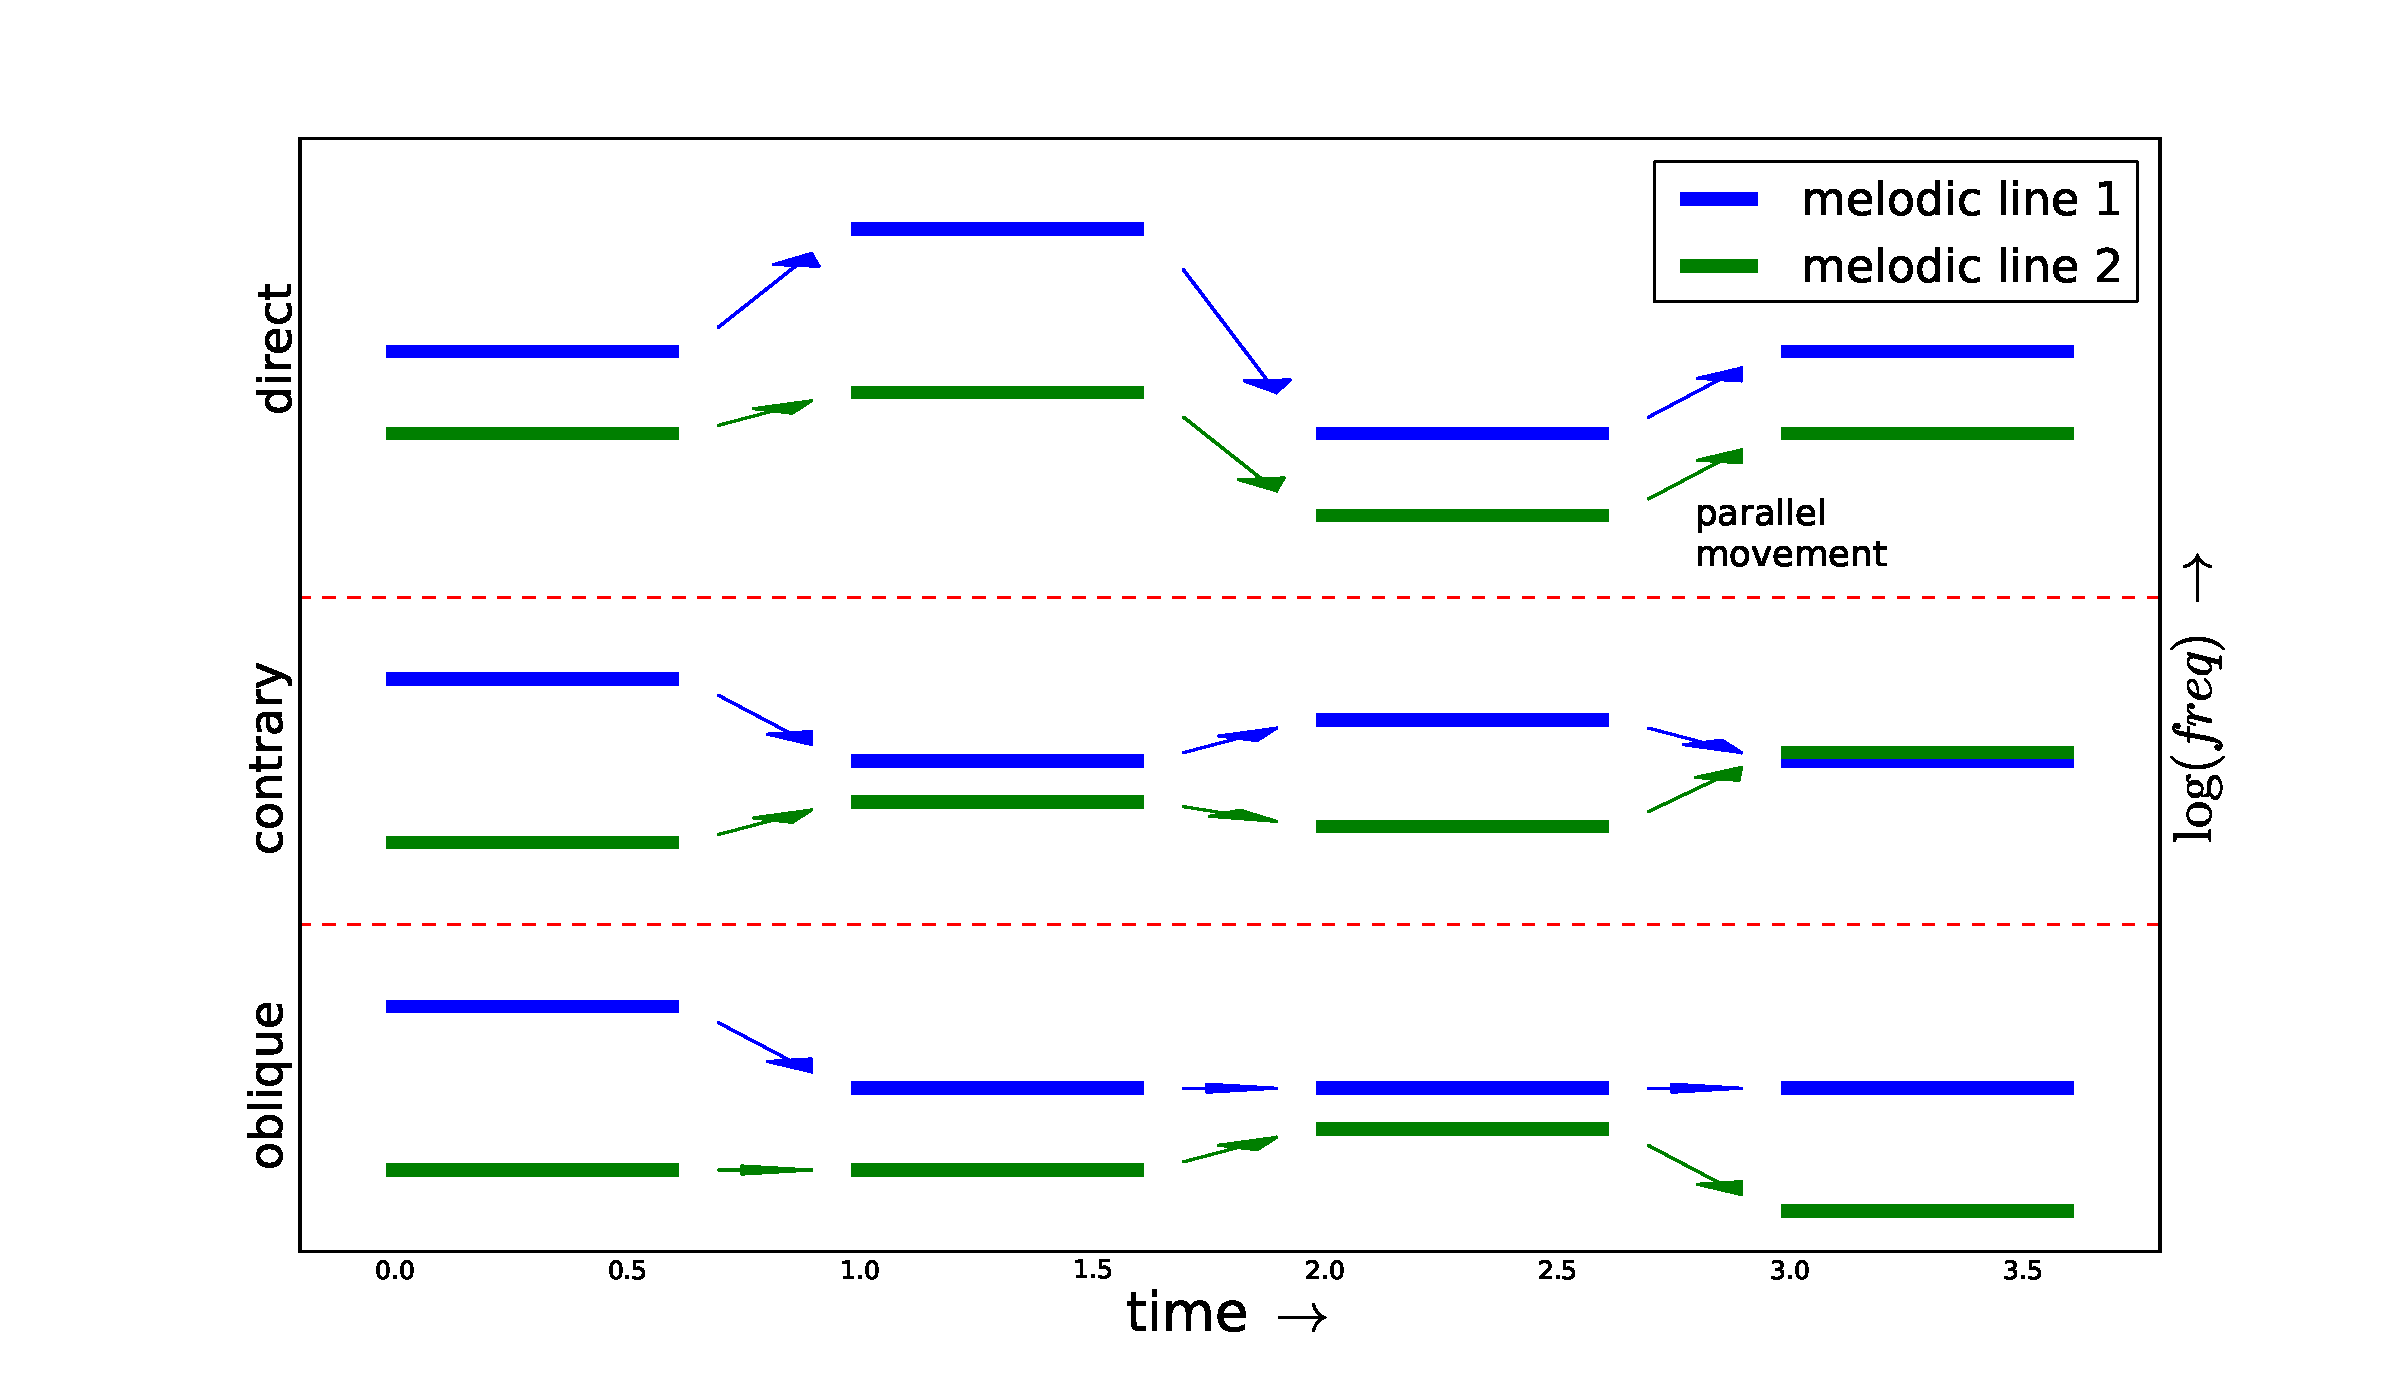
\includegraphics[width=\columnwidth]{figures/movContraponto}
    \caption{Different motions of counterpoint aiming to preserve independence
        between voices. There are 3 types of motions: direct, contrary and
        oblique. The parallel motion is a type of direct motion.}
        \label{fig:movContraponto}
\end{figure}

The purpose of counterpoint is to conduct voices in a way they sound
independent. In order to do that, the relative motion of voices (in pairs), is crucial and
categorized as: direct, oblique and contrary motion (see Figure~\ref{fig:movContraponto}). The parallel motion is an oblique motion.
The gold rule here is to take care with the direct motions, avoiding making them
lead to a perfect consonance. The parallel motion should occur only between
imperfect consonances and no more than three consecutive times. The dissonances
can be unadmitted or used when followed and preceded by consonances of joint
degrees, i.e.\ neighbor notes in a scale. The motions that lead a note to a
neighbor sound more coherent. When having 3 or more voices, the melodic
importance lies on the higher and lower voices, in this particular
order~\cite{Fux,Tragtenberg,SchoenbergContra}.

These rules were used in the music piece \emph{Conta ponto}, the source code is
in Appendix~\ref{ap:conta} and available online in \massa.

\subsection{Rhythm}\label{subsec:ritmo}

Basically speaking, the rhythm notion is dependent on events separated by durations~\cite{Lacerda}. These events can be heard individually if spaced by at least $50-63ms$. To make the temporal separation between them be perceived as duration, the period should be large enough, around $100ms$~\cite{microsound}.  
It is possible to summarize the duration transitions heard as rhythm and pitch,
in the following way~\cite{Alfaix, microsound}.

\begin{table*}[htpq!]
\tiny
\centering
\caption{Transition of durations heard individually until it turns into pitch.}
\begin{tabular}{  l | r r r r   r r r    r r r || r r || r r r r r r }
\hline
           & \multicolumn{10}{c}{$\underleftarrow{\text{\bf perception zone of
           duration as rhythm}}$} & \multicolumn{2}{c}{transition} & \multicolumn{3}{c}{-} \\
duration (s) & {\bf ...}     & {\bf 32,}     & {\bf 16,}   & {\bf 8,}  & {\bf 4,}   & {\bf 2,}   & {\bf 1,}   & {\bf 1/2,} & {\bf 1/4,} & {\bf 1/8,} & $\frac{1}{16}=62,5ms$ , & $\frac{1}{20}=50ms$ & {\color{gray} 1/40} & {\color{gray} 1/80  } & {\color{gray} 1/160 } & {\color{gray} 1/320 } & {\color{gray} 1/640 } & {\color{gray} ... } \\
frequency (Hz) & {\color{gray} ...} & {\color{gray} 1/32,}   & {\color{gray} 1/16,} & {\color{gray} 1/8,} & {\color{gray} 1/4,} & {\color{gray} 1/2,} &  {\color{gray} 1,}  & {\color{gray} 2,}   & {\color{gray} 4,}   & {\color{gray} 8,}    & 16,  & 20   & {\bf 40}   & {\bf 80}   & {\bf 160}   & {\bf 320}   & {\bf 640}   & {\bf ...} \\
           & \multicolumn{10}{c}{ - } & \multicolumn{2}{c}{transition}
           & \multicolumn{6}{c}{$\overrightarrow{\text{\bf perception zone of
           duration as pitch}}$} \\
\hline
\end{tabular}
\label{tab:duracoes}
\end{table*}

The duration region marked as transition is presented minimized because the limits
are not well defined. In fact, the duration where someone begins to perceive a
fundamental frequency or a separation between occurrences, depends on the
listener and sound characteristics~\cite{microsound,Roederer}. 

The rhythmic metric is commonly based on a basic duration called pulse. The
pulse typically comprehends durations between $0.25-1.5s$ ($240$
and $40 BPM$, respectively). In music education and cognitively studies, it is common to
associate these range of pulse frequencies to the durations of the heart beat,
movements of inspiration and expiration and walk steps~\cite{Lacerda,Roederer}.

The pulse is subdivided into equal parts and repeated in sequence. These
relations (division and concatenation) usually follow relations of small
order integers\footnote{In ascending order of occurrence in written and ethnic
music, these indicate the musical pulse divisions and their sequential grouping at
time: 2, 4 and 8, after that 3, 6 (two groups of 3 or 3 groups of 2) and 9 and
12 (three and 4 groups of 3). At last, the prime numbers 5 and 7, complementing
1-9 and 12. Other metrics are less common, like divisions and grouping in 13,
17, etc, and are mainly used in contexts of experimental music and classical
music of XX and XXI. No matter how complex they seem, metrics are commonly
compositions and decompositions of 1-9 equal parts~\cite{Gramani,Roederer}.}.
A schematic exposition is shown in Figure~\ref{fig:pulsoSubAgl}.

\begin{figure}[h!]
    \centering
        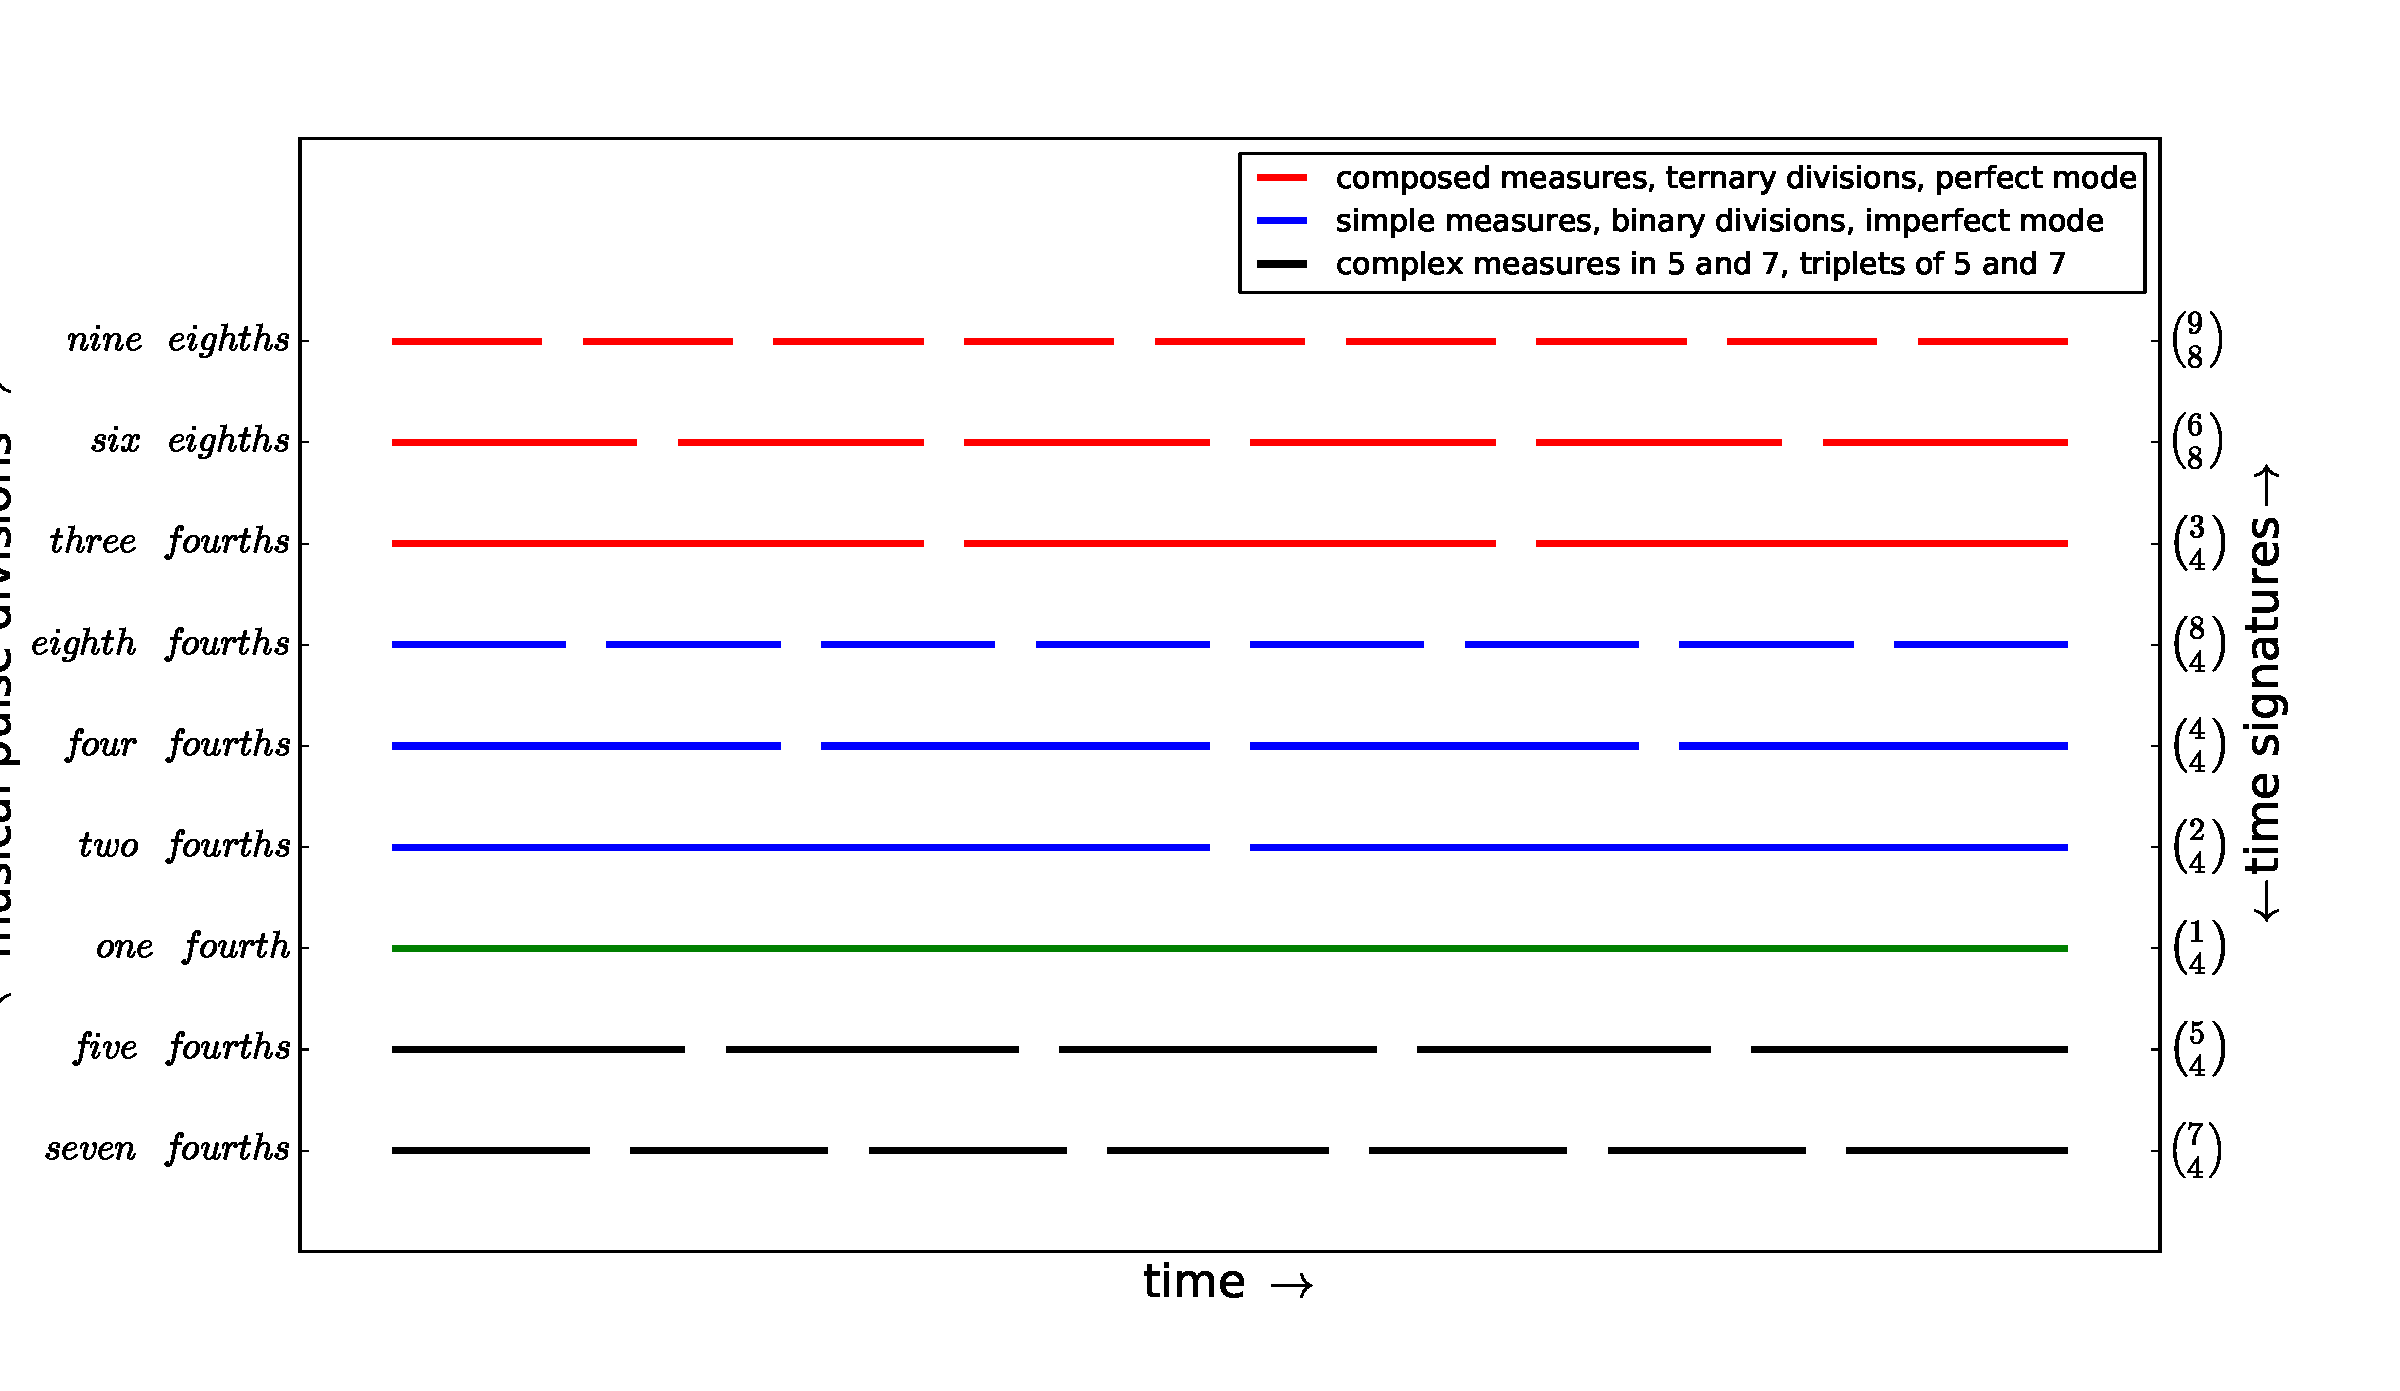
\includegraphics[width=\columnwidth]{figures/metricaMusical}
    \caption{Divisions and grouping in bars for the music pulse to establish a rhythmic
        metric. Divisions of the quarter note, established as the
        pulse, is presented in the left. The time signature whose specifies the same
        metrics but having as scale the groupings of the music pulse is presented in the right.}
        \label{fig:pulsoSubAgl}
\end{figure}

Dual relations (common time and binary divisions) are frequent in dance rhythms
and celebrations. Ternary relations are common in
ritualistic music and is related to the sacred. Dual relations are called imperfect, while and the ternary relations are called perfect.

The strong unities (accents) are the ones that fall in the 'head' of bars, the downbeats. The
head of a unity is the first part of the subdivision. In binary divisions (2, 4
and 8, for example), the unities originally strong turn into weak (não sei se isso ficou claro)
(e.g.\ division in 4 is: strong, weak, strong medium, weak). In ternary divisions
(3, 6 and 9) two weak unities succeeds the downbeat (e.g.\ division in 3 is:
strong, weak, weak)\footnote{Division in 6 is considered compound but can also
occur as a binary division. A binary division which suffers a ternary division
results in two units divided in tree units each: strong (subdivided in strong,
weak, weak) and weak (subdivided in strong, weak, weak). Another way to perform
the division in 6 is applying ternary division that suffers a binary division,
resulting in: a strong unit (subdivided in strong and weak) and two weak units
(subdivided in strong and weak for each).}

The accent in the weak beat is known as the backbeat, whereas a note starting in a weak
beat which duration coming across the strong beat is known as syncope.

Notes can occur inside and outside of these \emph{'music metric'} divisions. In
most behaved cases, notes occur exactly on these divisions, with broader
incidence on attacks of strong beats.
In extreme cases, the time metric cannot be perceived~\cite{Roederer}. 
Small grid variations help to build musical interpretation and differences
between styles~\cite{Cook}.

% ficou um tanto confuso:

Being pulse the grouping level $j=0$, level $j=-1$ the first pulse subdivision,
level $j=1$ the first pulse agglomeration and so on. In this way, $P_i^j$ is the
$i$-th unit of pulses at grouping level $j$: $P^0_{10}$ is the tenth pulse,
$P^{1}_3$ is the third pulse grouping unit (and, possibly, the third measure),
$P^{-1}_2$ is the second unit of pulse subdivision.

Special attention should be given to the limits of $j$: pulse divisions are
durations sensible as rhythm. Furthermore, the pulse joints sums, at its
maximum, a music or a cohesive set of musics. In other words, a duration given
by $P^{min(j)}_i$, $\forall \; i$, is greater than $50 ms$ and the durations
summed together $\sum_{\forall i}P^{\text{max}(j)}_i$ are less than a few
minutes or at most, a few hours.

Each level $j$ has some indexes $i$. A index $i$ always has three different
values (or multiple of three) that occur in a perfect relation. When $i$ has only
multiple of two, four or eight different values, than an imperfect relation occurs,
as shown in Figure~\ref{fig:pulsoSubAgl}.

Any unit (note) of a given musical sequence which has a time metric can be unequivocally
specified as:

\begin{equation}
P^{ \{ j_k \} }_{ \{ i_{k} \}}
\end{equation}

\noindent where $j_k$ is the grouping level and$i_k$ is the unit order itself.

As example, consider $P^{-1,0,1}_{3,2,2}$ as the third subdivision $P^{-1}_3$ of the
second pulse $P^0_2$ and of the second pulse group $P^1_2$. Each unit or unit set
$P_i^j$ can be associated with a sequence of temporal samples $T_i$ that forms a
music note.

The music piece \emph{Poli Hit Mia} explorers different metrics (avaleble in Appendix~\ref{ap:poli} and as part of \massa).


\subsection{Repetition and variation: motifs and large units}\label{subsec:motivos}

Given the basic music structures, either frequential (chords and scales) or
rhythmic (beat divisions and simple, compound and complex grouping), it is
natural to organize these structures in a cohesive way~\cite{Boulez}. To this end,
the concept of arcs are fundamental: we make an arc by departing from a place (music unit) and going to another one. The audition of melodic and harmonic lines is pervaded as
musical arcs thanks to the cognitive nature of the musical hearing. It is
possible to consider the note as the smaller arc, and each motif (definir motif aqui? nao foi falado ainda) and melody as another arc. Each time, beat subdivision, measure and music
section constitutes an arc. A music in which the arcs do not present consistency by
themselves, can be understood as a music with no cohesion. The coherence feeling
comes, mostly, from the skilled manipulation of arcs in a music piece.

Musical arcs are abstract structures and liable of basic operations. An spectral
arc, like a chord, can be inverted, enlarged and permuted, to cite some
examples. Temporal arcs, like a melody, a motif, a measure or a note are also
capable of variations. Remembering that
$S_j=\left\{s_j=T_i^j=\{t_i^{j}\}_0^{\Lambda_j-1}\right\}_0^{H-1}$ is a sequence
of $H$ musical events $s_j$, each event with its $\Lambda_j$ samples $t_i^j$
(refer to the beginning of this section~\ref{notasMusica}), the basic techniques
can be described as:

\begin{itemize}
        \item Temporal translation is a displacement
    $\delta$ of a specific material to another instant $\Gamma'=\Gamma + \delta$
    of the music. It is a variation that changes temporal localization in
    a music:
    $\left\{s_j'\right\}=\left\{s_j^{\Gamma'}\right\}=\left\{s_j^{\Gamma+\delta}\right\}$
    where $\Gamma$ is the duration between the beginning of the piece (or considered
    period) and the first event $s_0$ of original structure $S_j$. Observe that
    $\delta$ is the time offset of the displacement.

    \item Temporal expansion or contraction is a change in duration of each
    arc by a factor $\mu\,:\; s_j'^{\Delta}=s_j^{\mu_j . \Delta}$. Possibly,
    $\mu_j=\mu$ is constant.

    \item Temporal reversion consists of generating a sequence with elements
    in reverse order of the original sequence $S_j$, thus: $S_j'=\left\{s_j'\right\}_0^{H-1}=\left\{s_{(H-j-1)}\right\}_0^{H-1}$.

    \item Pitch translation is a displacement $\tau$ of a material for a
        different pitch $\Xi'=\Xi + \tau$. It is a variation that changes pitch
        localization of material:
        $\left\{s_j'\right\}=\left\{s_j^{\Xi'}\right\}=\left\{s_j^{\Xi+\tau}\right\}$
        where $\Xi$ is the pitch of a period $S_j$ or of an event $s_0$ of the
        original structure $S_j$. Observe that $\tau$ is the pitch offset of the
        displacement. If $\tau$ is given in semitones, the displacement in
        frequency is $\tau_f=f_0.2^{\frac{\tau}{12}}$ where $f_0$ results from
        the adoption of some reference: $f_0=\Xi_{f_0}Hz\;\sim \Xi_0$ absolute
        value of pitch. For the frequency of any pitch value: $\Xi_f=\Xi_{f_0}.2^{\frac{\Xi-\Xi_0}{12}}$. 
        For the pitch of any frequency value: $\Xi=\Xi_0 +12
        . \log_2\left(\frac{\Xi_f}{\Xi_{f_0}}\right)$.  
        In the MIDI protocol, $\Xi_{f_0}=55Hz$ while pitch $\Xi_0=33$ marks
        a \textit{A 1}, another reference point is $\Xi_{f_0}=440Hz$ which
        corresponds to $\Xi_0=69$. The unit difference is equal for semitones.
        It is not possible to say that the unit is the semitone because $\Xi=1$
        is not a semitone, but a note with an audible frequency as rhythm, with
        less than 9 occurrences each second (see Table~\ref{tab:duracoes}).

        \item Interval inversion is the inversion traversed by
        the material. The inversion is strict if the number of semitones is
        being used as a reference for the operation:
        $S_j'=\{s_j'\}_0^{H-1}=\left\{s_j^{-\varepsilon_j . f_0}\right\}$, where
        $\varepsilon_j$ is the factor between the event frequency $s_j$ and the
        frequency of $s_0$. The inversion is said tonal if the distances are
        considered in terms of degree number of the scale $E_k$:
        $S_j'=\{s_j'\}_0^{H-1}=\left\{s_j^{-\varepsilon^{\left(e_{\left(j_e\right)}\right)}
        . f_0}\right\}_0^{H-1}$ where $j_e=e_{j}^{inv}$ is the index $k=j_e$ in
        $E_k$ of the note of event $s_j$.

        \item Rotation of musical elements is the transference of the last
        element to the position of the first element, and the displacement of
        that to the penult, one position ahead. It is possible to define
        rotation of $\tilde{n}$ positions by $S'_n=S_{(n+\tilde{n})\%H}$. If
        $\tilde{n}<0$, it is enough to use $\tilde{n}'=H-\tilde{n}$. It is
        reasonable to associate $\tilde{n}>0$ with the clockwise rotation and
        $\tilde{n}<0$ with tne anti clockwise rotation. More information about rotations in presented in subsection~\ref{estCic}.

        \item The insertion and removal of materials into structure $S_j$ can be
    ornamental or structural: $S_j'=\{s_j'\}=\{s_j \text{ if condition A,
    otherwise } r_j\}$, for any music material $r_j$, including the empty
    instant. Elements of $R_j$ can be inserted at the beginning, like a prefix
    in $S_j$; at the end, as a suffix; or at the middle, dividing $S_j$ or making
    it the prefix or suffix. Both materials can be mixed in a variety of ways.

    \item Changes in articulation, orchestration and spatialization, 
    $s_j'=s_j^{*_j}$, where $*_j$ is the new characteristic incorporated by the
    element $s_j'$.
    
    \item Accompaniment. Both orchestration and melodic lines presented when
    $S_j$ occurs can suffer modifications and be considered as a variation of $S_j$ itself.
\end{itemize}

Other proceesings can be derived together with the presented ones, as, for example, the retrograde
inversion, temporal contraction with an external suffix, etc. The music
structures resound in the human cognitive system due to the own nature of
thought. In its many veneers, an idea read with the same number of elements and
connective aspects between them. The music, when tunned with those mental structures,
raises impressions. In this way, a whole process of mental and neurological
resonance is unleashed, responsible by the feelings, memories and imaginations,
typical to a mindful music listening. This cortical activity helps the
musical therapy, known by its utility in cases of depression and neurological
injury. It is known that regions of the human brain responsible by
hearing processing, are also used for other activities, even linguistic and mathematical~\cite{Sacks,Roederer}.

The paradigmatic structures guide the creation of new music material. One of the
most central of them is the dipole tension/relax. Traditional dipoles
are relate to tonic/dominant, repetition/variation,
consonance/dissonance, coherence/rupture, symmetry/asymmetry,
equality/difference, arrival/departure, near/far, stationary/moving,
etc. The ternary relations tend to relate to the circular and unification. The
lucid ternary communion, 'modus perfectus', opposes to the passionate
dichotomic, 'modus imperfectus'. Hereafter, there is an exposition dedicated to
directional and cyclic arcs.

%%%%%%%%%%%%%%%%%%%%%%%%%%%%%%%%%%%%%%%%%%%%


\subsection{Directional structures}\label{subsec:dir}

The arcs can be decomposed in two convergent sequences: the first arc reaches the
apex and the second arc returns from the apex to the start region. This apex is called climax by traditional music theory. It is
possible to differ between arcs whose climax are placed at the beginning, middle, end,
and at the first and second half of the considered duration. These structures are
shown in Figure~\ref{fig:climax}. The parameter of variation does not exist, thus
the arc consists only of the reference structure~\cite{Schoenberg}.

\begin{figure}[h!]
    \centering
        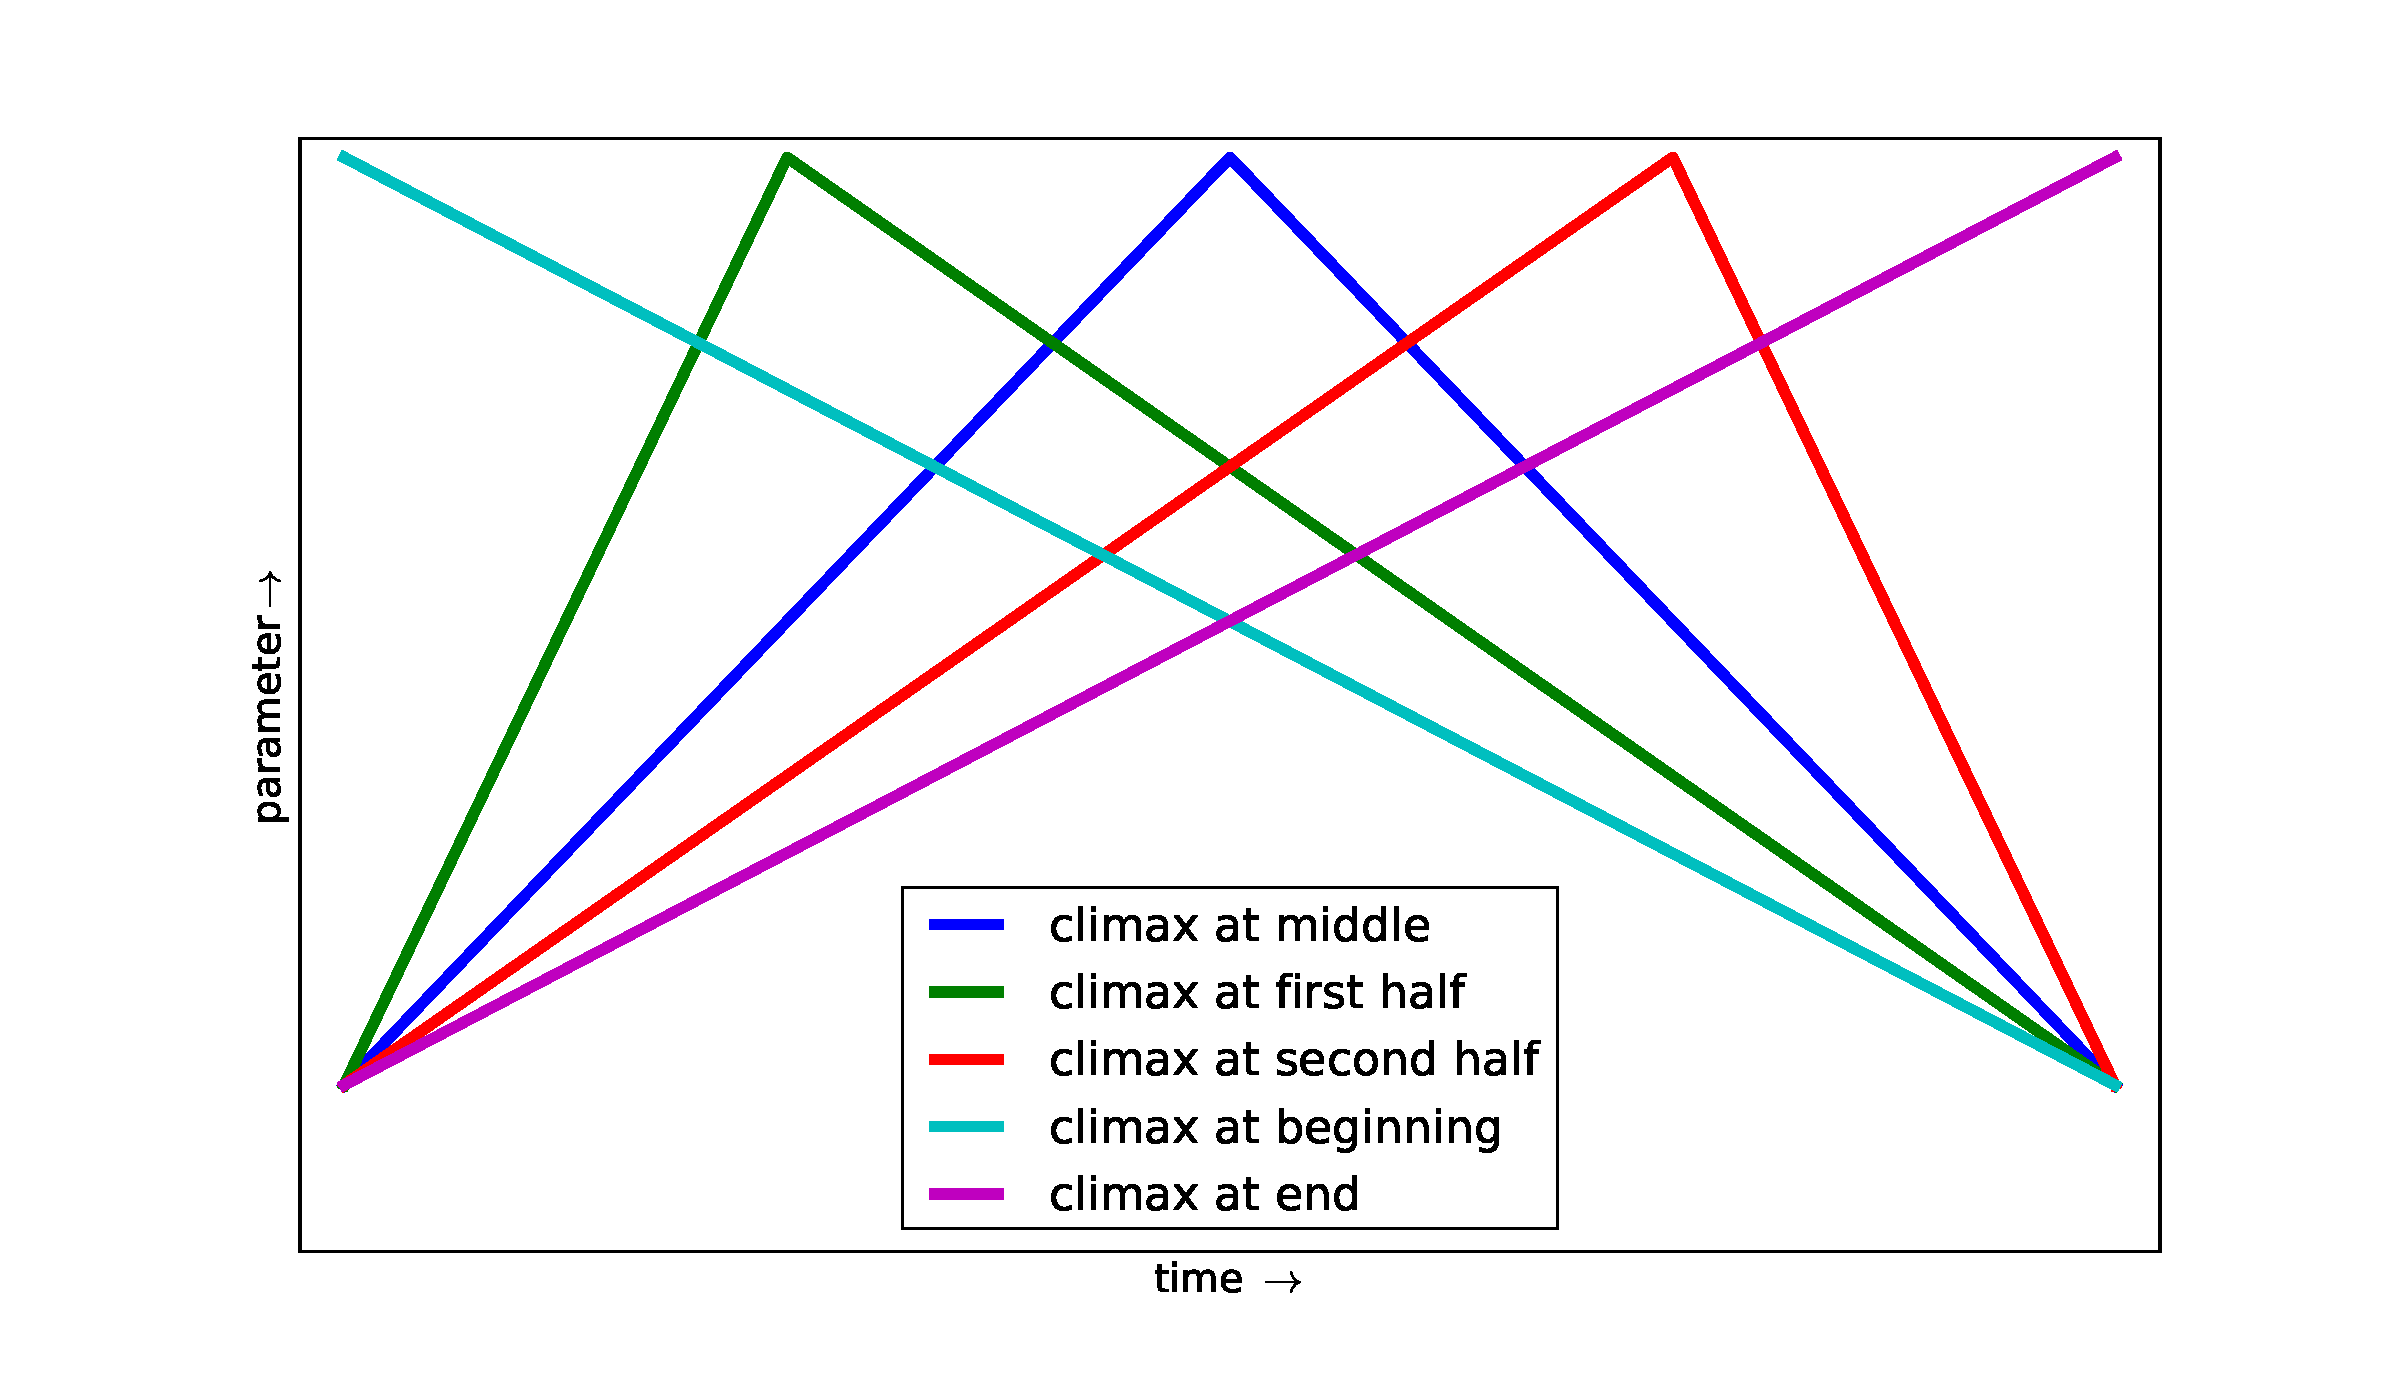
\includegraphics[width=\columnwidth]{figures/climax}
        \caption{Canonical distinctions of musical climax in a given melody and
        other domains. The considered possibilities are: climax at beginning,
        climax at first half, climax at middle, climax at second half and climax
        at the end. The y-axis is not properly specified since there exist no
        real parametric variation and, therefore, the structure is a reference.}
        \label{fig:climax}
\end{figure}

Consider $S_i=\{s_i\}_0^{H-1}$ as an increasing sequence. The sequence
$R_i=\{r_i\}_0^{2H -2}=\left\{s_{(H-1-|H-1-i|)}\right\}_0^{2H-2}$ is a sequence
that presents a perfect profiteer symmetry, i.e.\ the second half is the
mirrored version of the former. Following the musical concepts, the climax is
localized in the middle of the sequence. It is possible to modify this
fact using sequences with different sizes. All the mathematical theory of
sequences, already well established and taught routinely in calculus courses, can be
used to generate those arcs~\cite{Guidorizzo,Schoenberg}. 
Theoretically, when applied to any characteristic of music events, these sequences produce arcs, since they imply the deviation and return of an initial
parametrization. Henceforth, it is possible to have a
number of distinct arcs, with different sizes and climax for a same sequence of events. This is an interesting and useful resource, and the correlation of arcs results in coherence~\cite{Salzer}.

Historically (and practically nowadays), the golden ratio and the Fibonacci sequence have special importance. The Lucas sequence allows the generalization of
Fibonacci sequence, making it easy to understand. Given any two numbers $x_0$
and $x_1$, the Lucas sequence can be obtained as: $x_n=x_{n-1}+x_{n-2}$. The greater $n$ is, the more $\frac{x_{n}}{x_{n_1}}$ approaches the golden ratio:
$1.61803398875...$. The sequence converges fast even with high discrepant
initial values. Being $x_0=1$ and $x_1=100$, and $y_n=\frac{x_n}{x_{n+1}}$ an
auxiliary sequence, the error occurring in the first values with
relation to the golden ratio is, approximately, $\{ e_n \}
=\left\{100\frac{y_n}{1.61803398875}-100 \right\}_1^{10}=\{6080.33, -37.57, 23,
-7.14, 2.937, -1.09, 0.42, -0.1601, \\ 0.06125, -0.02338\}$. The Fibonacci sequence
presents about the same error progression but starts right at the second step since $\frac{1}{1}\approx\frac{101}{100}$.

The music piece \emph{Dirracional} exposes the use of arcs into directional structures.
Its source code is included in Appendix~\ref{ap:dirracional} and available online as part
of \massa~\cite{MASSA}.

\subsection{Cyclic structures}\label{estCic}

The philosophical understanding that the human thought is based on the perception of
similarities, differences, stimuli and objects, places the symmetries
at the core of the cognitive process~\cite{Deleuze}. Mathematically, symmetries
are algebraic finite groups, and a finite group is always isomorphic to a permutation
group. It is possible to say that permutations represent any symmetry in a
finite system (precisa de uma referência aqui). In music, permutations are ubiquitous and considerably present in techniques, which confirms their central role. The successive application of permutations generates cyclic arcs~\cite{change,Zamacois,permMusic}. Two academic studies were dedicated to this end, aiming at generating music structures~\cite{figgusOriginal, figgusEspacializacao}.

Any permutation set can be used as a generator of algebraic groups~\cite{permMusic}.
The properties defining a group $G$ are:

\begin{multline}\label{eq:groups}
%\begin{split}
\forall \;\; p_1,p_2 \in G \Rightarrow\quad\;\; p_1 \bullet p_2  =
p_3 \in G \\ \;\;\;\text{(closure property)} \\
\forall \;\; p_1,p_2,p_3 \in G \Rightarrow\quad (p_1\bullet p_2)\bullet p_3  =
p_1\bullet (p_2\bullet p_3)\quad\;  \\ \text{(associativity property)} \\
\exists \;\; e \in G :\; p \bullet e  = e \bullet
p \;\;\;\; \forall p \in G  \quad \\ \text{(identity element property)} \\
\forall \;\; p \in G, \;\exists\; p^{-1} :\quad\;  p\bullet p^{-1} 
=p^{-1}\bullet p = e \\ \; \text{(inverse element property)}
%\end{split}
\end{multline}

From the first property it is possible to conclude that any permutation can be
operated with another permutation. In fact, it is possible to apply a
permutation $p_1$ and another permutation $p_2$, and, comparing both initial and final
orderings, results in another permutation $p_3$.

Every element $p$ operated with itself a sufficient number of times $n$ reaches
the identity element $p^n=e$ (otherwise the group would be infinite, generated
by $p$). The lower $n\;:\;p^n=e$ is called the element order. Thus, a finite
permutation $p$, successively applied, reaches the initial ordering of its
elements, making a cycle. This cycle, if used as parameter of music notes,
implies in a cyclic musical arc.

These arcs can be established by using a set of different permutations. As a historic
example, the tradition called \emph{change ringing} conceives the music through
bells played one after other and then played again, but in a different
order. This process repeats until it reaches the initial ordering. The set of
different traversed orderings is a \emph{peal}. Table~\ref{tab:change}
represents one traditional \emph{peal} for 3 bells (1, 2 and 3) which explores
all possible orderings. Each line indicates one bell ordering to be
played. Permutations occur between each line. In this case, the music structure
consists of permutations by itself and some different permutations operate due to
the cyclic behavior.

\begin{table}[htpq!]
\centering
\caption{Change Ringing: Standard \emph{peal} for 3 bells. Permutations
occur between each line. Each line is a bell ordering and each ordering is played
        a line a time.} 
\begin{tabular}{l c r}
\textcolor{red}{1} & \textcolor{blue}{2} & \textcolor{green}{3} \\
\textcolor{blue}{2} & \textcolor{red}{1} & \textcolor{green}{3} \\
\textcolor{blue}{2} & \textcolor{green}{3} & \textcolor{red}{1} \\
\textcolor{green}{3} & \textcolor{blue}{2} & \textcolor{red}{1} \\
\textcolor{green}{3} & \textcolor{red}{1} & \textcolor{blue}{2} \\
\textcolor{red}{1} & \textcolor{green}{3} & \textcolor{blue}{2} \\
\textcolor{red}{1} & \textcolor{blue}{2} & \textcolor{green}{3}
\end{tabular}
\label{tab:change}
\end{table}

The use of permutations in music can be summarized in the following way:
consider $S_i=\{s_i\}$ as a sequence of musical events $s_i$ (e.g.\ notes), and a
permutation $p$. $S_i'=p(S_i)$ comprises the same elements of $S_i$ but in a
different order. The permutations can be written based on two notations: cyclic or
natural. The natural notation basically comprehends the order of the resulting indexes from
the permutation. Thus, agreed the original ordering given the sequence of its
indexes $[0\;1\;2\;3\;4\;5\;...]$, the permutation is noted by the sequence it
produces (ex. $[1\;3\;7\;0\;...]$). In the cyclic notation, permutation is the
changing of one element by the posterior one, and the last element by the first one.

It is not necessary to permute elements of $S_i$, but only some
characteristics. In this way, being $p^f$ a permutation in frequency and $S_i$ a
sequence of basic notes as exposed in the end of section~\ref{notaBasica}, the
new sequence $S_i'=p^f(S_i)=\left\{s_i^{p(f)}\right\}$ consists of the same
music notes, respecting same order and maintaining the same characteristics, but with the
fundamental frequencies permuted following the pattern that $p^f$ presents.

It is worthwhile to mention two subtleties of this procedure. First, the permutation $p$ does not have to involve all elements of $S_i$, i.e.\ it can operate in subsets of $S_i$. Second,  the elements $s_i$ do not have to be entirely executed at each state access. To exemplify,
consider $S_i$ as a sequence of music notes $s_i$. If $i$ goes from $0$ to $n$, and
$n>4$, at each measure of $4$ notes it is possible to execute the first $4$
notes. The other notes of $S_i$ can occur in measures where permutations set
aside those notes to the first four notes of $S_i$.

Each one of the permutations $p_i$ described above relates the note dimensions where it operates (frequency, duration, \emph{fades},
intensity, etc) and the period of incidence (at how much access a permutation is
applied). During realization of notes in $S_i$, an easy and coherent form is to
execute the first $n$ notes\footnote{The execution of disjoint notes of $S_i$
equals to modify the permutation and to execute the first notes.}.

Appendix~\ref{cap:FIGGUScode} and \massa present the computational implementation about permutations~\cite{MASSA,figgusOriginal,figgusEspacializacao}.

\subsection{Musical idiom?}

There are many studies intending to model and explore a 'musical language',
or 'linguistics applied to music' or even to discern between different 'musical
idioms'~\cite{Lerdahl, Harmonia, Salzer,Alfaix}. In a simple way, a musical idiom
is the result of a chosen material together with repetition of elements and
repetition of relations between elements present along the music. The related dichotomies are outstanding, as explained at subsection~\ref{subsec:motivos}: repetition and variation, relax and tension, equilibrium and instability, consonance and dissonance, etc.

\subsection{Musical usages}\label{subsec:usosmusicais3}

The basic note was defined and characterized in quantitative terms (section~\ref{sec:notaDisc}). Next, the internal note
composition was addressed and both internal transitions and immediate treatment
were understood (section~\ref{varInternas}). Finally, this section aims at
organizing these notes in music. The gamma of resources and consequent infinitude
of possibilities is a typical situation and highly relevant for art contexts~\cite{Harmonia,Webern}.

There are studies dedicated to each one of the presented resource. For example, it is possible to obtain the 'dirty' triadic harmonies (with notes without the triad) by
superpositions of dirty fourths. Another interesting example is the simultaneous
presence of rhythms in different metrics, constituting what is
called \emph{polyrhythms}. The music piece \emph{Poli-hit mia} explores these
simultaneous metrics by impulse train (??) convolved with notes that compound the
line. Its source code is included in Appendix~\ref{ap:poli} and available online as part
of \massa.

The microtonal scales are important for the music of the 20th
century~\cite{microtonalidade} and present diverse outstanding results, like the
fourths of tone in the Indian music. The musical sequence \emph{MicroTom}
explores these resources, including microtonal melodies and microtonal harmonies
with many notes in a very reduced note scope. Its code is presented in
Appendix~\ref{ap:micro} and available online in \massa.

As pointed in subsection~\ref{subsec:mus2}, the relations between
parameters are powerful ways to acquire music pieces. The number of permuted
notes can vary during the music, revealing relationship with piece
duration. Harmonies can be made of triads (eqs.~\ref{triades}) with replicated
notes at each octaves and more numerous as minor the depth and frequency of
vibratos (eqs.~\ref{vbrGamma},~\ref{vbrAux},~\ref{vbrF},~\ref{vbrGamma2},~\ref{vbrT}),
among other uncountable possibilities.

The presented symmetries at octave divisions (eqs.~\ref{escSim}) and the
symmetries presented as permutations (Table~\ref{tab:change} and
eqs.~\ref{eq:groups}) can be used together. In the music piece \emph{3 trios}
this association is done in a systematic way in order to enable the required
listening. This is a instrumental piece, not included as a source
code~\cite{3Trios}. 

The \emph{PPEPPS} (Pure Python EP: Projeto Solvente) is an EP synthesized using
the resources presented in this study. With minimal parametrization, the program
generates complete musics, allowing the easy composition of musics and sets of
musics. Using few lines of code it is possible to obtain
a directory with the generated musics. This facility and technological
demystification create aesthetically possibilities for both sharing and education.



%%%%%%%%%%%%%%%%%%%%%%%%%%%%%%%%%%%%%%%%%%%%%%%%%%%%%%%%%%%%%%%%%%%%%%%%%%%%%%%
%%%%%%%%%%%%%%%%%%%%%%%%%%%%%%%%%%%%%%%%%%%%%%%%%%%%%%%%%%%%%%%%%%%%%%%%%%%%%%%
%%%%%%%%%%%%%%%%%%%%%%%%%%%%%%%%%%%%%%%%%%%%%%%%%%%%%%%%%%%%%%%%%%%%%%%%%%%%%%%
%%%%%%%%%%%%%%%%%%%%%%%%%%%%%%%%%%%%%%%%%%%%%%%%%%%%%%%%%%%%%%%%%%%%%%%%%%%%%%%
%%%%%%%%%%%%%%%%%%%%%%%%%%%%%%%%%%%%%%%%%%%%%%%%%%%%%%%%%%%%%%%%%%%%%%%%%%%%%%%
%%%%%%%%%%%%%%%%%%%%%%%%%%%%%%%%%%%%%%%%%%%%%%%%%%%%%%%%%%%%%%%%%%%%%%%%%%%%%%%

\section{Conclusions and future works} %Nome do capítulo.
\label{cap:conclusao}

We have described a concise system that explores the musical elements and relate them to the digital signal. The reader is invited to access \emph{Scripts} and \massa, where these relations are computationally implemented. We hope the didactic report along the paper and the supplied scripts facilitates and encourages the use of the proposed framework. 

The open possibilities provided by the techniques and results discussed in this paper involve psychoacoustic experiments and the creation of interfaces for the generation of music, noise and other music applications in a high fidelity (\emph{hi-fi}). It is worthwhile to mention the benefit of these results for artistic and didactic purposes. The incorporation of programming skills is facilitated by the provided visual aids. Initial \emph{live-coding} practices and guided courses based on this work have already been realized with successful. Examples are Puredata and Chuck.

This work systematically investigates the parameterization issues (like the tremolo, ADSR, etc.) in a high fidelity, which has significant artistic utility. Such detailed analytical descriptions, together with the computational implementations, have not been covered before in the literature (as shown in Appendix~\ref{cap: trabalhosRelacionados}). 

Besides, the free software license and online availability of the exposed content as hypertext, in conjunction with the respective codes and sound examples, strongly facilitates future collaborations and the generation of sub-products in a co-authorship fashion. As consequence, the expansion of \massa is feasible and straightforward, making it possible new developments and implementations of musical context.

In addition, this work permitted the formation of groups with common interests, like music creativity and computer music. Specially, the project \url{labMacambira.sf.net} groups Brazilian and foreign co-workers in order to offer relevant contributions in diverse areas like Digital Direct Democracy (não devo ter traduzido certo), georeferencing techniques, artistic and educational activities. Some of these reports are available in Appendix~\ref{cap:musicaExtra} and made online. There are more than 700 videos, written documentations, original softwares and contributions in well-known external softwares such as Firefox, Scilab, LibreOffice, GEM/Puredata, to name a few~\cite{siteLM,wikiLM,vimeoLM}.       

Future works include the application of the reported results in machine learning and artificial intelligence methods for the generation of appealing artistic materials. 


%% Há um aumento no número de pesquisas relacionadas à música em andamento no campus de São Carlos da USP, o que sugere facilidade para estabelecer parcerias.
%% As publicações acadêmicas efetivadas durante este mestrado também apontam para uma multidisciplinaridade,
%% tratando diretamente de questões humanas como artes, filosofia, humor e linguagem falada e escrita, através de artifícios lineares e estatísticos.\cite{FabbriSTAT,FabbriACL,FabbriComplenetVoz,FabbriComplenetTexto} Os desdobramentos estão alcançando redes sociais e teorias epistemológicas com base em pesquisas prévias, dos orientadores deste trabalho, com forte presença de redes complexas e processamento de linguagem natural. 


\nocite{*}
\bibliography{article}
\end{document}
